% Options for packages loaded elsewhere
\PassOptionsToPackage{unicode}{hyperref}
\PassOptionsToPackage{hyphens}{url}
%
\documentclass[
]{article}
\usepackage{amsmath,amssymb}
\usepackage{lmodern}
\usepackage{iftex}
\usepackage{skak}
\ifPDFTeX
  \usepackage[T1]{fontenc}
  \usepackage[utf8]{inputenc}
  \usepackage{textcomp} % provide euro and other symbols
\else % if luatex or xetex
  \usepackage{unicode-math}
  \defaultfontfeatures{Scale=MatchLowercase}
  \defaultfontfeatures[\rmfamily]{Ligatures=TeX,Scale=1}
\fi
% Use upquote if available, for straight quotes in verbatim environments
\IfFileExists{upquote.sty}{\usepackage{upquote}}{}
\IfFileExists{microtype.sty}{% use microtype if available
  \usepackage[]{microtype}
  \UseMicrotypeSet[protrusion]{basicmath} % disable protrusion for tt fonts
}{}
\makeatletter
\@ifundefined{KOMAClassName}{% if non-KOMA class
  \IfFileExists{parskip.sty}{%
    \usepackage{parskip}
  }{% else
    \setlength{\parindent}{0pt}
    \setlength{\parskip}{6pt plus 2pt minus 1pt}}
}{% if KOMA class
  \KOMAoptions{parskip=half}}
\makeatother
\usepackage{xcolor}
\IfFileExists{xurl.sty}{\usepackage{xurl}}{} % add URL line breaks if available
\IfFileExists{bookmark.sty}{\usepackage{bookmark}}{\usepackage{hyperref}}
\hypersetup{
  hidelinks,
  pdfcreator={LaTeX via pandoc}}
\urlstyle{same} % disable monospaced font for URLs
\usepackage{longtable,booktabs,array}
\usepackage{calc} % for calculating minipage widths
% Correct order of tables after \paragraph or \subparagraph
\usepackage{etoolbox}
\makeatletter
\patchcmd\longtable{\par}{\if@noskipsec\mbox{}\fi\par}{}{}
\makeatother
% Allow footnotes in longtable head/foot
\IfFileExists{footnotehyper.sty}{\usepackage{footnotehyper}}{\usepackage{footnote}}
\makesavenoteenv{longtable}
\usepackage{graphicx}
\makeatletter
\def\maxwidth{\ifdim\Gin@nat@width>\linewidth\linewidth\else\Gin@nat@width\fi}
\def\maxheight{\ifdim\Gin@nat@height>\textheight\textheight\else\Gin@nat@height\fi}
\makeatother
% Scale images if necessary, so that they will not overflow the page
% margins by default, and it is still possible to overwrite the defaults
% using explicit options in \includegraphics[width, height, ...]{}
\setkeys{Gin}{width=\maxwidth,height=\maxheight,keepaspectratio}
% Set default figure placement to htbp
\makeatletter
\def\fps@figure{htbp}
\makeatother
\setlength{\emergencystretch}{3em} % prevent overfull lines
\providecommand{\tightlist}{%
  \setlength{\itemsep}{0pt}\setlength{\parskip}{0pt}}
\setcounter{secnumdepth}{-\maxdimen} % remove section numbering
\ifLuaTeX
  \usepackage{selnolig}  % disable illegal ligatures
\fi

\author{}
\date{}

\begin{document}

Mario Leoncini

ELEMENTI

DI STRATEGIA

NEGLI SCACCHI

\_\_\_\_\_\_\_\_\_\_\_\_\_\_\_\_\_\_\_\_\_\_\_\_\_\_\_\_

1992. Prima edizione su carta 2004

\textbf{INTRODUZIONE}

Se la tattica è lo sfruttamento combinativo di una debolezza e la
tecnica è la capacità di vincere una partita considerata vantaggiosa, la
strategia è il piano di gioco.

Qualcuno, in modo divertente quanto efficace, ha sintetizzato la
differenza tra strategia e tattica dicendo: \emph{``La tattica è sapere
che cosa fare quando c'è qualcosa da fare e la strategia è sapere che
cosa fare quando non c'è niente da fare''.}

La buona accoglienza riservata a questo scritto, nato alla fine del 1992
in forma di lezioni per ``Mc link'', il BBS della nota rivista di
informatica ``McMicrocomputer'', mi ha indotto a raccogliere il
materiale e ampliarlo in un libro. Libro che si occupa di strategia e
più in particolare degli elementi rilevanti per la formulazione del
piano di gioco. La strategia ha per scopo la formazione di debolezze
tali da poter essere sfruttate con colpi tattici o in sede tecnica.

La sua formulazione deve naturalmente tener conto di tutti gli elementi
presenti sulla scacchiera che però, beninteso, varia al variare della
posizione. Non è quindi possibile formulare un piano unico valido per
tutte le stagioni ma è anche vero che, data una posizione, talvolta
possono formularsi più piani. La scelta del piano dipende allora
dall'indole del giocatore ma non si possono formulare piani che non
tengano conto degli elementi strategici presenti nella posizione.

Un altro errore comune è credere che la differenza tra un maestro e un
principiante risieda nella capacità di calcolo; certo, un bravo
giocatore è capace di calcolare con precisione anche lunghe varianti; ma
la superiorità è soprattutto di ordine strategico. Il maestro \emph{sa}
che cosa fare in qualsiasi posizione senza bisogno di calcoli
approfonditi. La formulazione di un piano riduce drasticamente la
necessità del calcolo delle varianti; in questo senso nel corso della
partita il maestro può calcolare meno di un principiante ma vincere lo
stesso. È per questo che i forti giocatori possono giocare contro molti
avversari contemporaneamente in simultanea e batterli.

In verità, chiunque giochi a scacchi, fosse anche alle primissime armi,
dà al proprio gioco almeno un simulacro di strategia. Nella versione più
semplice essa consiste nel domandarsi, dopo ogni mossa dell'avversario:

1) se il proprio materiale è minacciato e si è sotto minaccia di scacco
matto; se la risposta a questa domanda è sì, allora

1,1) porvi rimedio; altrimenti

2) vedere se si può, a nostra volta, minacciare materiale o il matto.

Per ragionare in questi termini occorre naturalmente conoscere il valore
dei pezzi.

Se si prende come unità di misura il pedone, il loro valore è, grosso
modo, questo: Donna~=~9, Torre = 5, Alfiere = 3, Cavallo = 3.

Ecco dunque che lo studio degli elementi strategici è anche lo studio
dei fattori che vanno considerati, oltre al materiale, per capire chi è
in vantaggio data una qualsiasi posizione. Di più: non solo il materiale
non è l'unico elemento, come può esserlo in giochi più semplici degli
scacchi, ma il suo valore è "relativo", varia a seconda della
disposizione degli altri pezzi.

Questo libro può essere letto da chi già conosce le regole e ha un
minimo di esperienza ma si rivolge, in particolare, a quel vasto settore
di giocatori che desiderano migliorare il proprio gioco e che sono
collocati tra la terza categoria sociale e il titolo di candidato
maestro. Costoro sono soliti commettere l'errore di tralasciare lo
studio della strategia in favore di quello delle aperture. Non nego che
lo studio delle aperture (e dei finali, anch'essi spesso immeritatamente
trascurati) sia indispensabile, ma rischia di trasformarsi in inutile
esercizio mnemonico se non si capiscono i motivi che si nascondono
dietro le successioni di mosse, presentate, nei monumentali libri tipo
``Enciclopedia'' di Belgrado, in forma inevitabilmente asettica.

Ci sono giocatori che entrano in profonda crisi, e che commettono gli
errori più incredibili, quando, nella variante d'apertura preferita, il
loro avversario esegue una mossa non studiata o non contemplata dai
``sacri'' testi. Questi giocatori troveranno qui raccolti, e spiegati in
modo sistematico, elementi che hanno cominciato a intravedere e intuire
fin dalle prime partite.

La loro conoscenza e il loro studio sono gli indispensabili ingredienti
per un gioco di livello magistrale.

Mario Leoncini 1992--1996

\textbf{I -- SVILUPPO DEI PEZZI E PERDITA DI TEMPI}

Molti di voi sapranno già che la partita suole dividersi in tre fasi ben
distinte: apertura, mediogioco e finale.

L'apertura è caratterizzata dallo ``sviluppo'' dei pezzi. Tengo qui a
sottolineare un primo concetto non spiegato a sufficienza in molti
manuali. Per \emph{sviluppo} non si intende il semplice spostamento dei
pezzi dalle loro case iniziali, piuttosto conferire ad essi \emph{una
funzione}. È ovvio che di norma per conferire ad un pezzo una funzione
occorre muoverlo, ma non di necessità.

Ogni manuale illustra invece a dovere l'importanza del centro: per
rendersi conto di quanto sia importante occupare con i pezzi le case
centrali basta riflettere che, per esempio, un Cavallo posto in una
delle quattro case centrali può andare in una casa d'angolo in due o tre
mosse mentre un Cavallo posto in una casa d'angolo impiega per andare in
un'altra casa d'angolo cinque o sei mosse. Chi ha i pezzi raggruppati
nella zona centrale può spostare in meno che non si dica forze ingenti
in ogni parte della scacchiera.

È ovvio che non è facile occupare il centro con i pezzi; i pezzi sono
facilmente scacciabili dai pedoni e finché ci sono pedoni arretrati
questa operazione è impossibile.

Nella fase iniziale della partita si assiste allora ad una lotta per lo
spazio centrale. Di solito i giocatori spingono al centro i pedoni in
modo da sviluppare indisturbati i propri pezzi nelle retrovie oppure
lasciano all'avversario la possibilità di occuparlo con i pedoni per poi
minarlo con spinte oculate.

Tipiche difese che contemplano questa strategia sono la Alekhine e la
Grünfeld.

Vediamo le prime mosse di entrambe:

\emph{Alekhine:} \textbf{1.e4 ¤f6 2.e5 ¤d5 3.c4} (una variante meno
pretenziosa è 3.d4) \textbf{3... ¤b6 4.d4 d6 5.f4}

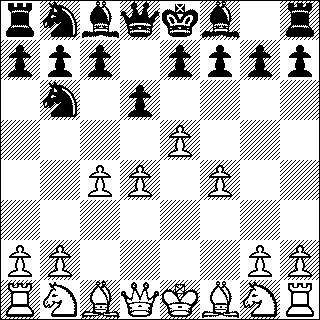
\includegraphics[width=1.50417in,height=1.50417in]{vertopal_109f12be458a423d8f3cc838880eaea2/media/image1.png}\emph{diagramma
1}

\emph{Grünfeld:} \textbf{1.d4 ¤f6 2.c4 g6 3.¤c3 d5 4.¤xd5 ¤xd5 5.e4 ¤xc3
6.bxc3}

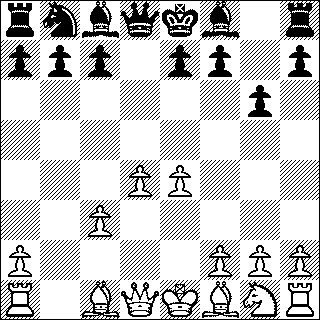
\includegraphics[width=1.50417in,height=1.50417in]{vertopal_109f12be458a423d8f3cc838880eaea2/media/image2.png}\emph{diagramma
2}

In queste difese il Bianco è teso a comprimere l'avversario e a
sfruttare il vantaggio di spazio; il Nero lavora ai fianchi per minare
la struttura di pedoni nemica. Se ci riesce il crollo del centro ha di
solito effetti dirompenti perché potrà essere occupato da pezzi che non
potranno essere in alcun modo scacciati. \emph{"Ogni spinta di pedone
crea una debolezza"} ammoniva Steinitz.

Un altro elemento da tener presente è la velocità di mobilitazione delle
forze. Negli scacchi non si esce con un pezzo per fare azioni
dimostrative, saggiare la reazione del nemico e agire di conseguenza,
non se ne avrebbe il tempo! Si mobilitano invece le forze prima
possibile. Per fare questo si deve evitare di muovere senza necessità lo
stesso pezzo in apertura (andare in due mosse in una casa in cui si può
andare in una si dice ``perdere un tempo'').

Per sapere nelle prime mosse d'apertura chi è in vantaggio di sviluppo
c'è un metodo molto semplice: fare la conta dei pezzi sviluppati. Si sa
che il Bianco, avendo la prima mossa, è in vantaggio. In linea generale
dovrebbe riuscire a terminare la mobilitazione delle forze prima del
Nero.

Ammettiamo che le prime mosse di una partita siano \emph{1.e3 e5 2.e4} e
si noti che la stessa posizione si ottiene dopo \emph{1.e4 e5} ma con la
mossa al Bianco. Nel caso in esame è invece il Nero che può completare
lo sviluppo per primo e dopo \emph{2... ¤f6} egli ha già un pezzo
sviluppato contro nessuno del Bianco. In altre parole è bastato un solo
tempo perso per far passare il vantaggio (lieve quanto si vuole ma
innegabile) dal Bianco al Nero.

Per capire meglio questo concetto vediamo due esempi tratti dalla teoria
delle aperture.

\textbf{1.e4 e5 2.¤f3 ¤c6 3.¥b5} (Partita Spagnola)

\emph{diagramma 3}

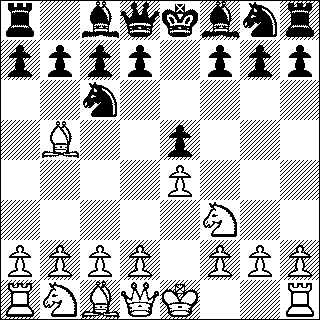
\includegraphics[width=1.50417in,height=1.50417in]{vertopal_109f12be458a423d8f3cc838880eaea2/media/image3.png}

Questa è una buona mossa perché fa pressione sullo schieramento del Nero
sul lato di Donna. L'Alfiere in b5 è sì attaccabile dal pedone
avversario (per esempio con 3... a6) ma senza guadagno di tempo: dopo
\textbf{3... a6 4.¥a4} il Bianco ha ancora due pezzi sviluppati contro
uno solo del Nero.

Questo ci dà modo di chiarire il concetto: si ha guadagno di tempo solo
quando un pezzo è costretto a muoversi perché attaccato da un altro
pezzo o da un pedone centrale (mossa che, di solito, è utile all'uscita
dei pezzi. Di per sé i pedoni si muovono non si sviluppano!).

Quando il Nero gioca 3... a6 il Nero fa più o meno questo ragionamento:
``Tu hai messo l'Alfiere in una posizione che comprime il mio lato di
Donna. Non mi piace per niente e intendo scacciarti, ma non subito, solo
quando lo decido io. Ora io gioco 3... a6 e ti costringo a scegliere tra
una delle seguenti possibilità:

a) a cambiare l'¥b5 con 4.¥xc6 ma allora rimango con il vantaggio dei
due Alfieri.

b) a spostarlo in a4 per continuare a esercitare la stessa pressione. In
tal caso però io sono pronto, quando lo riterrò opportuno, a scacciarti
con una semplice spinta di pedone (b7-b5).''

Dopo 3... a6 4. ¥a4 di solito a questo punto il Nero gioca \textbf{4...
¤f6}; non c'è infatti necessità di spingere subito in b5. Se il Bianco
avesse voluto prendere in c6 l'avrebbe fatto alla mossa precedente. Ora
sì che questa mossa sarebbe una perdita di tempo. Il Nero infatti,
rispetto a una mossa fa, ha mosso un Cavallo.

\emph{Difesa Scandinava:} \textbf{1.e4 d5 2.exd5 £xd5 3.¤c3!}

\emph{diagramma 4}

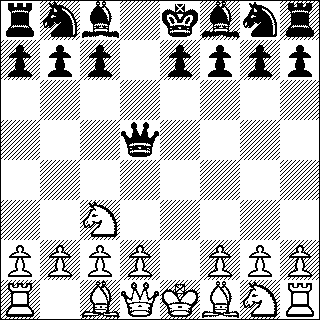
\includegraphics[width=1.50417in,height=1.50417in]{vertopal_109f12be458a423d8f3cc838880eaea2/media/image4.png}

Questa mossa invece guadagna un tempo sul serio: costringe la Donna a
muoversi ancora e permette al Bianco di continuare lo sviluppo. Anche da
questo esempio traiamo un importante insegnamento: occorre attenzione
nel piazzare la Donna in apertura perché non potendo essere facilmente
barattata è costretta a muoversi ogni volta che incroci pezzi nemici.

La gravità della perdita di tempi non è costante ma dipende dal
carattere della posizione; se è chiusa, intendendo con questo termine
posizioni dove catene di pedoni dividono i due schieramenti, tale
perdita è meno grave. Nelle posizioni ``chiuse'' si assiste spesso a
manovre interne tese a portare i pezzi a contatto con i punti deboli
dell'avversario (gioco posizionale). Ne consegue che se un giocatore si
trova in vantaggio di sviluppo (caso tipico è quello di averlo già
completato mentre l'avversario ha ancora qualche mossa prima di poter
arroccare) allora deve aprire il gioco cambiando pedoni a tutta forza,
specie se centrali. Quanto più il vantaggio di sviluppo è marcato tanto
più è opportuno aprire le linee anche a costo di sacrificare materiale.
La forza d'urto della guerra lampo era già nota agli scacchisti prima
che Hitler nascesse!

Per finire vediamo una partita giustamente celebre in cui Paul Morphy,
mettendo in pratica questi semplici principi, acquisisce in poche mosse
un vantaggio decisivo e chiude con una combinazione brillante.

Morphy--Duca Karl e Conte Isouard, Parigi 1858.

\textbf{1.e4 e5 2.¤f3 d6} difende in e5. Questa mossa, che dà origine
alla Difesa Philidor è del tutto giocabile anche se non così buona come
la naturale 2... ¤c6 che pareggia il numero dei pezzi sviluppati.

\textbf{3. d4} il Bianco apre le linee per permettere uno sviluppo
arioso. Se ora il Nero prende in d4 (3... exd4) si priva del suo unico
baluardo centrale. In caso di presa ci si potrebbe chiedere come
riprendere il Pedone. Vale la pena soffermarci a riflettere che in
questa posizione esso potrà essere ripreso anche di Donna. Infatti la
casa d4 è meno esposta agli attacchi di quel che sembra. Scartato subito
l'attacco di pedone c7-c5 perché indebolisce in modo grave il Pd6 e crea
un ``buco'' in d5, il Bianco risponderebbe a 4... .¤c6 con 5. ¥b5! e se
5... .¥d7 6. ¥xc6 ¥xc6 7.¤c3 e i tre pezzi sviluppati (contro uno solo
del Nero) e l'occupazione delle case centrali ben compensano la rinuncia
alla coppia degli Alfieri. Non del tutto a torto molti preferiscono
anteporre, dopo 1.e4 e5 2.¤f3 d6 3.d4 exd4 4.£xd4, l'uscita d'Alfiere in
d7 alla mossa di Cavallo in c6.

\textbf{3... ¥g4} sembra una buona mossa ma non lo è. Il Nero difende il
Pe5 inchiodando il Cavallo e sviluppando un pezzo. In apparenza ha
ristabilito la parità nello sviluppo dei pezzi (uno per uno) ma \ldots{}

\textbf{4.£xe5 ¥xf3} forzata. Il Nero è costretto a privarsi dell'unico
pezzo sviluppato. Si consideri che la posizione è ``ariosa'' e che in
tali circostanze la coppia degli Alfieri è un bene cui non si rinuncia
senza compensi di altro genere; e qui non si vede che cosa il Nero abbia
ottenuto in cambio.

\textbf{5.£xf3 £xe5 6.¥c4 ¤f6 7.£d3} il Bianco rimuove la Donna per
piazzarla in una casa dove sviluppa la sua massima efficacia. Non si può
parlare di perdita di tempo perché le minacce su f7 e b7 costringono il
Nero a difendersi senza poter muovere un pezzo leggero.

\textbf{7... £e7} per poter rispondere a 8.£xb7 con 8... £d4+, cambiare
le Donne e tirarla in lungo.

Esaminiamo la posizione: sia il Bianco che il Nero hanno mosso due pezzi
ma che differenza! Quelli bianchi sono piazzati in case ideali mentre la
Donna nera intralcia lo sviluppo sul lato di Re e il Nero dovrà
necessariamente rimuoverla, con pe¢dita di tempi.

\textbf{8.¤c3!} ecco una mossa che all'epoca solo Morphy poteva giocare.
Altri avrebbero preso in b7 e dopo 8... £d4+ 9.c3 ¥c5 avrebbero forse
anche vinto ma dopo un lungo finale. Morphy capisce che non è il momento
di andare a caccia di pedoni ma di incrementare il vantaggio di
sviluppo.

\textbf{8... c6} non avendo più lo scacco in b4 il Nero difende il Pb7
ma questa è ancora una mossa di pedone.

\textbf{9.¥g5} ormai il vantaggio di sviluppo è schiacciante. Quattro
pezzi già piazzati nelle case migliori, le torri pronte ad entrare in
gioco tramite la colonna d. Per contro il Nero ha solo due pezzi mossi e
uno di essi dovrà essere rimosso perché impedisce lo sviluppo.

\textbf{9... b5 10.¤xb5} in queste condizioni il sacrificio è così
spontaneo che non abbisogna nemmeno di un calcolo preciso: non può
essere sbagliato!

\textbf{10... ¤xb5 11.¥xb5+ ¤bd7 12.0-0-0} l'attacco si sviluppa da sé.

\textbf{12... ¦d8}

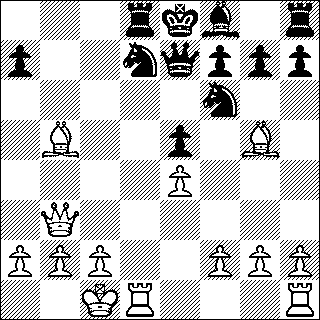
\includegraphics[width=1.50417in,height=1.50417in]{vertopal_109f12be458a423d8f3cc838880eaea2/media/image5.png}

\emph{diagramma 5}

La partita è strategicamente vinta. Ora non rimane che il colpo tattico.

\textbf{13.¦xd7! ¦xd7 14.¦d1 £e6 s}e il nero invece di giocare 14...
.£e6 avesse mosso la Donna in d8 il Bianco avrebbe vinto con: 15.¥xd7+;
infatti:

\begin{enumerate}
\def\labelenumi{\alph{enumi})}
\item
  15. ... ¢e7 16.£a3 (o £d4) matto;
\item
  15. ... ¤xd7 16.¥xd8 ¢xd8 17.£d3 come se non bastasse, cade anche il
  Cavallo;
\item
  15. ... £xd7 16.¦xd7 anche non considerando che l'attacco non è ancora
  finito, il vantaggio di materiale del Bianco è più che sufficiente per
  vincere: due pedoni in più, un terzo (il \textbf{§}a7) indifendibile e
  la Donna vale di più di Alfiere e Torre.
\end{enumerate}

\textbf{15.¥xd7+ ¤xd7 16.£d8+!! ¤xb8 17.¦d8 matto.}

Come questa partita dimostra, la combinazione è la naturale conclusione
di una partita vinta innanzitutto dal punto di vista strategico.

A Morphy bastava applicare semplici concetti quali lo sviluppo e il
guadagno dei tempi, contro avversari che non li conoscevano ancora, per
terminare la partita con combinazioni spettacolari. La superiorità di
Morphy non risiedeva nella tattica, come si crede' a lungo, ma nella
strategia; la tattica non fu che un inevitabile corollario di questa
superiorità strategica.

\textbf{II -- UN METODO PER AVVANTAGGIARSI IN APERTURA: IL GAMBETTO}

Nella prima lezione abbiamo parlato del rapido sviluppo e del guadagno
di tempi in apertura. Un metodo comune per guadagnare tempi si ha
sacrificando materiale, di norma un pedone. Il sacrificio di pedone per
avvantaggiarsi nello sviluppo o guadagnare spazio sulla scacchiera si
chiama gambetto. Il termine fu usato per la prima volta da Ruy Lopez nel
trattato \emph{``Libro de la invencion liberal y arte del juego de
¥xedrez''} del 1561 e deriva dall'italiano (gamba, sgambetto).

Di solito è il Bianco a sacrificare un pedone per incrementare quel
lieve vantaggio che gli deriva dal diritto alla prima mossa ma sono
stati elaborati numerosi gambetti anche per il Nero.

Per capire la filosofia del gambetto si veda questo esempio:

\emph{Partita Italiana:} \textbf{1.e4 e5 2.¤f3 ¤c6 3.¥c4 ¥c5 4.c3} scopo
di questo tratto è di spingere successivamente in d4 per piazzare al
centro due pedoni.

\textbf{4... ¤f6 5.d4}

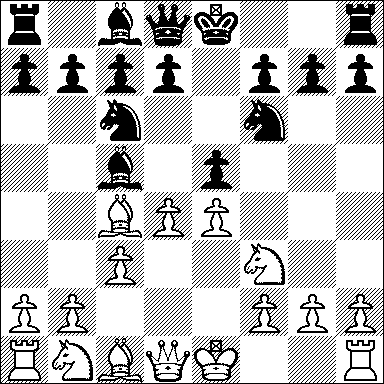
\includegraphics[width=1.40139in,height=1.40139in]{vertopal_109f12be458a423d8f3cc838880eaea2/media/image6.png}\emph{diagramma
6}

Il Bianco ha spinto un secondo pedone al centro. Sostenuto com'è dal
\textbf{§}c3 esso non potrà facilmente essere rimosso. Per ottenere
questo indubbio vantaggio ha però dovuto giocare due mosse di pedone in
apertura e il Nero ne ha approfittato per continuare lo sviluppo con
4... ¤f6.

Nel 1824, un lupo di mare, il capitano di marina William Davies Evans
ideò una continuazione che raggiungeva la stessa configurazione (c3, d4,
e4) senza che il Nero si fosse avvantaggiato nello sviluppo (4... ¤f6).
Naturalmente non si poteva raggiungere l'obiettivo senza dare nulla in
cambio; nacque così un interessante sacrificio di pedone:

\emph{Gambetto Evans:} \textbf{1.e4 e5 2.¤f3 ¤c6 3.¥c4 ¥c5 4.b4} ecco la
mossa di Evans; \textbf{4... ¥xb4 5.c3 ¥c5 6.d4}

\emph{diagramma 7}

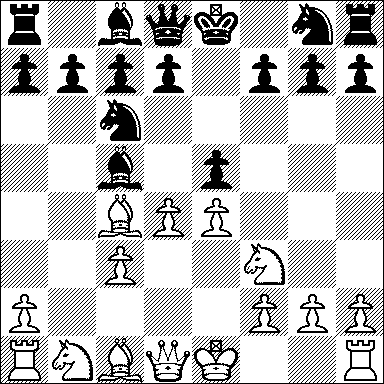
\includegraphics[width=1.40972in,height=1.40972in]{vertopal_109f12be458a423d8f3cc838880eaea2/media/image7.png}

Si confronti questa posizione con quella derivante dalla Partita
Italiana. Il Bianco non ha più il pedone b2 ma il Cavallo nero si trova
ancora nella casa di partenza (g8).

Naturalmente, se ora togliessimo tutti i pezzi dalla scacchiera il Nero
vincerebbe il finale in virtù del pedone in più ma \emph{``prima del
finale gli dei hanno creato il centro partita''} recita un celebre
aforisma di Tartakower.

È importante riflettere che negli scacchi il valore dei pezzi non è
assoluto ma solo indicativo: esso varia a seconda della loro
disposizione sulla scacchiera. Il controllo di una colonna o di una
diagonale possono valere quanto un pedone o più. Per intenderci un
Alfiere che controlla sette case vale di più di uno che ne controlla
solo due e un sacrificio è giustificato se serve a dare maggiore forza
ai pezzi rimanenti. È chiaro che alla fine quel che conta, a meno di non
dare matto, è il materiale che, prima o poi, deve essere recuperato, se
possibile con gli interessi, pena la perdita della partita.

Nel secolo scorso, quando le tecniche difensive non erano sofisticate
come lo sono oggi, i gambetti erano di gran moda; oggi hanno perso molto
del loro smalto ma non sono scomparsi dalla pratica dei tornei.
Piuttosto è cambiata l'idea che ne è alla base. Un tempo essi venivano
giocati per aggredire senza compromessi il Re avversario, oggi li si
gioca per ottenere vantaggi di o¢dine posizionale da far fruttare
a£dirittura in finale.

È ovvio che l'offerta di pedone può essere rifiutata. Chi l'accetta se
ne assume gli inevitabili rischi senza illudersi di arrivare facilmente
ad un finale vinto.

Se in risposta ad un gambetto il Nero gioca a sua volta un gambetto, si
parla di controgambetto. Alcuni manuali usano, a mio avviso meno
correttamente, il termine controgambetto per gambetto giocato dal Nero.

La rivista inglese ``Gambit'' ha classificato oltre trecento gambetti.
Oltre all'Evans, eccone altri tra i più giocati.

\textbf{1. Sacrifici operati dal Bianco}

\emph{Gambetto di Re:} \textbf{1.e4 e5 2.f4}

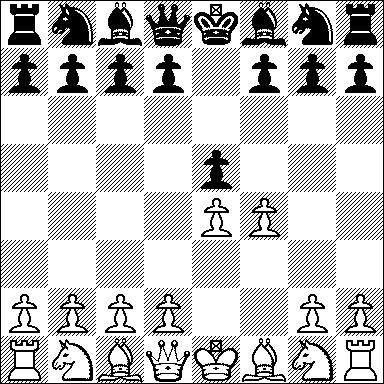
\includegraphics[width=1.40972in,height=1.40972in]{vertopal_109f12be458a423d8f3cc838880eaea2/media/image8.png}\emph{diagramma
8}

Il Gambetto di Re, considerato a buon diritto il Re dei gambetti perché
in voga da oltre cinque secoli è ancora oggi perfettamente giocabile. In
caso di accettazione del pedone (2... exf4), il Bianco ottiene di poter
piazzare un secondo pedone al centro (d2-d4) e di aprire la colonna
``f'' alla Torre. Dopo l'arrocco corto e la rimozione del §f4 il Bianco
potrà fare pressione su f7 che, essendo difeso solo dal Re, è il punto
più debole dello schieramento nero.

\textbf{2... exf4 3.h4} il Bianco mina il pedone f4 per sfruttare la
colonna f. Altre buone continuazioni sono: 3.¥c4 e 3.d4.

\emph{Gambetto Danese:} \textbf{1.e4 e5 2.d4 exd4 3.c3 £xc3 4.¥c4}

\emph{diagramma 9}

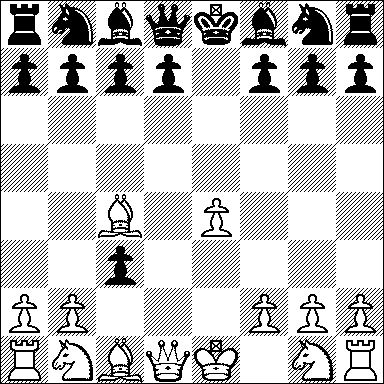
\includegraphics[width=1.40972in,height=1.40972in]{vertopal_109f12be458a423d8f3cc838880eaea2/media/image9.png}

Il Bianco sacrifica addirittura due pedoni pur di aprire il maggior
numero di linee.

Difficile dimostrare la correttezza di questi sacrifici ma al Nero è
richiesto un gioco attento ed ene¢gico.

Vediamo un possibile seguito:

\textbf{4... ¤xb2 5.¥xb2 d5!} l'idea del Nero, con questa forte reazione
centrale, è quella di restituire entrambi i pedoni per superare le
difficoltà d'apertura.

\textbf{6.¥xd5 ¤f6 7.¥xf7+ ¢xf7 8.£xd8 ¥b4+ 9.£d2 ¥xd2+ 10.¤xd2 ¦e8} e
il Nero non ha più nulla da temere.

\emph{Gambetto Scozzese:} \textbf{1.e4 e5 2.¤f3 ¤c6 3.d4 exd4 4.¥c4}

\emph{diagramma 10}

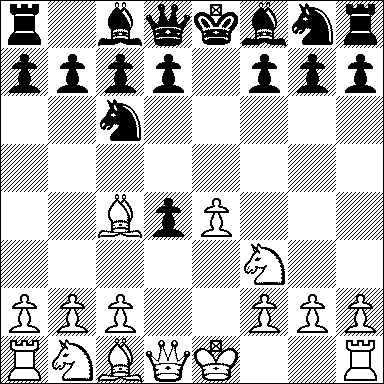
\includegraphics[width=1.40972in,height=1.40972in]{vertopal_109f12be458a423d8f3cc838880eaea2/media/image10.png}

Questo gambetto, già citato nei manoscritti di Gioacchino Greco (XVII
secolo) è stato in anni recenti arricchito di nuove idee e lo si può
incontrare anche in tornei di alto livello.

\emph{Gambetto Siciliano:} \textbf{1.e4 c5 2.b4}

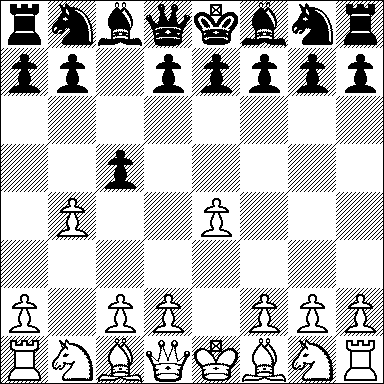
\includegraphics[width=1.40972in,height=1.40972in]{vertopal_109f12be458a423d8f3cc838880eaea2/media/image11.png}

\emph{diagramma 11}

Questa mossa, già citata in un manoscritto del 1623, è giocata solo
sporadicamente a livello magistrale. Sergio Mariotti ne ha fatto ogni
tanto uso per sorprendere gli avversari. Ecco un possibile seguito:

\textbf{2... ¤xb4 3.a3 bxa3?!} è meglio 3... d5!, una mossa buona per
controbattere molti gambetti.

\textbf{4.¤xa3 d6 5.¥b2 ¤f6 6.¥c4 ¤c6 7.£e2 g6 8.f3 ¥g7 9.d4 0-0 10.0-0}
e il Bianco ha compenso per il pedone sacrificato.

\emph{Gambetto Morra:} \textbf{1.e4 c5 2.d4}

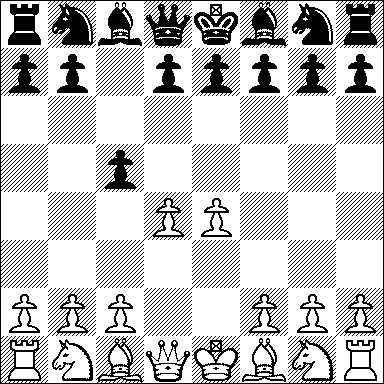
\includegraphics[width=1.40972in,height=1.40972in]{vertopal_109f12be458a423d8f3cc838880eaea2/media/image12.png}\emph{diagramma
12}

Questo gambetto conduce a scontri violenti in cui non è agevole per il
Nero tenere sotto controllo la situazione.

\textbf{2... ¤xd4 3.c3 £xc3} l'offerta può essere rifiutata senza
svantaggi sia con 3... d5 che con 3... ¤f6.

\textbf{4.¤xc3 ¤c6 5.¤f3 e6 6.¥c4 d6 7.0-0 ¤f6 8.£e2 ¥e7 9.¦d1} con
iniziativa.

\textbf{2. Sacrifici operati dal Nero}

\emph{Gambetto Albin:} \textbf{1.d4 d5 2.c4 e5}

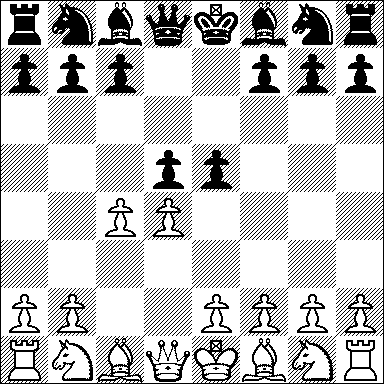
\includegraphics[width=1.40972in,height=1.40972in]{vertopal_109f12be458a423d8f3cc838880eaea2/media/image13.png}\emph{diagramma
13}

Tentativo violento, ma non del tutto corretto, di conquistare
l'iniziativa.

\textbf{3.£xe5 d4 4.¤f3} sarebbe un grave errore 4.e3? ¥b4+! 5.¥d2 £xe3
6.fxe3 \emph{(6.¥xb4? exf2+ 7.¢e2 fxg1=}\textbf{¤}\emph{+! 8.¢e1 £h4+
9.¢d2 ¤c6 10.¥c3 ¥g4 e vince)} 6... £h4+ 7.g3 £e4 8.£f3 ¥xd2+ 9.¤xd2
£xe5 con vantaggio del Nero.

\textbf{4... ¤c6 5.g3} preparandosi a piazzare l'Alfiere sulla grande
diagonale per fare pressione sul futuro arrocco lungo del Nero.

\textbf{5... ¥g4 6.¥g2 £d7 7.0-0 0-0-0} una mossa importante: prepara la
futura apertura della colonna h con le spinte h5-h4.

Però nello scontro violento che questa posizione configura la pratica ha
dimostrato che in genere l'attacco del Bianco arriva prima.

\emph{Gambetto di Budapest:} \textbf{1.d4 ¤f6 2.c4 e5}

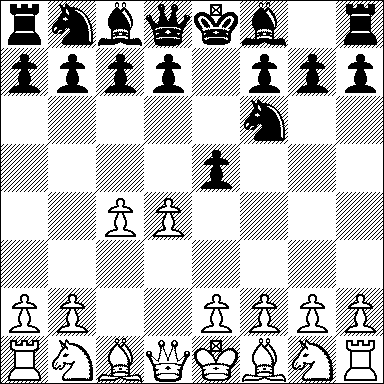
\includegraphics[width=1.40972in,height=1.40972in]{vertopal_109f12be458a423d8f3cc838880eaea2/media/image14.png}\emph{diagramma
14}

Pur non essendo del tutto giustificata questa coraggiosa spinta di
pedone, anche in tempi recenti, ha fatto registrare alcune belle
vittorie.

\textbf{3.£xe5 ¤g4} un'altra possibilità è 3... ¤e4 (Variante
Fajarowicz) in cui il Nero rinuncia alla pressione su d5 per puntare di
più sull'attacco.

\textbf{4.¥f4 ¤c6 5.¤f3 ¥b4+ 6.¤bd2 £e7 7.a3 ¤gxe5 8.¤xe5} non 8.axb4??
per 8... ¤d3 matto!

\textbf{8... ¤xe5 9.e3 ¥xd2+ 10.£xd2 d6} e il Bianco può contare sulla
coppia degli Alfieri.

\emph{Gambetto From:} \textbf{1.f4 e5}

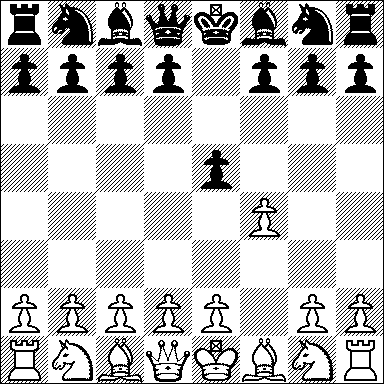
\includegraphics[width=1.40972in,height=1.40972in]{vertopal_109f12be458a423d8f3cc838880eaea2/media/image15.png}\emph{diagramma
15}

Chi spinge in e5 deve esser pronto a rientrare nel Gambetto di Re nel
caso venga giocata 2.e4.

\textbf{2.fxe5 d6 3.exd6 ¥xd6} notare che dopo appena tre mosse il Nero
minaccia già lo scacco matto (4... £h4+ 5.g3 ¥xg3+ 6.hxg3 £xg3 matto).

\textbf{4.¤f3 g5 5.d4 g4}

\emph{Gambetto Jaenisch:} \textbf{1.e4 e5 2.¤f3 ¤c6 3.¥b5 f5}

Questa variante della Partita Spagnola fu ideata dal maestro russo Karl
Jaenisch (1813-1872). Il gambetto sembra giustificato in caso di
accettazione del sacrificio.

\emph{diagramma 16}

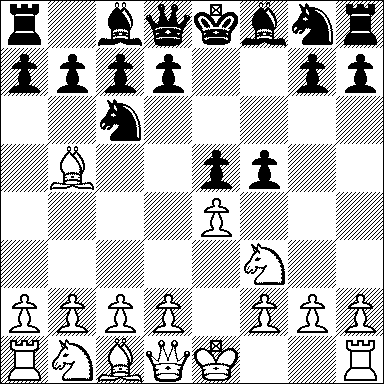
\includegraphics[width=1.40972in,height=1.40972in]{vertopal_109f12be458a423d8f3cc838880eaea2/media/image16.png}

\textbf{4.exf5 e4 5.£e2 £e7 6.¥xc6 £xc6 7.¤d4 £e5 8.¤f3 £xf5} il Nero
non esce male dalle schermaglie iniziali però il Bianco può rifiutare
l'offerta con la forte replica 4.¤c3! che porta a situazioni molto
complicate in cui è spesso il Nero a rimetterci le penne.

\emph{Attacco Marshall:} \textbf{1.e4 e5 2.¤f3 ¤c6 3.¥b5 a6 4.¥a4 ¤f6
5.0-0 ¥e7 6.¦e1 b5 7.¥b3 0-0 8.c3 d5}

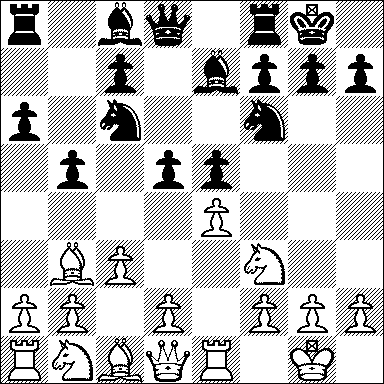
\includegraphics[width=1.40972in,height=1.40972in]{vertopal_109f12be458a423d8f3cc838880eaea2/media/image17.png}

\emph{diagramma 17}

Il campione americano Frank Marshall tenne per ben nove anni questa idea
``nel cassetto'', in attesa di giocarla in un incontro importante.
L'occasione gliela diede Capablanca a New York nel 1918. Come se nulla
fosse il geniale cubano trovò lì per lì la continuazione ancora oggi
ritenuta migliore e vinse la partita. Il gioco del Nero è stato
successivamente migliorato e oggi questo gambetto è una delle armi più
temibili contro la Partita Spagnola.

\textbf{9.exd5 ¤xd5 10.¤xe5 ¤xe5 11.¦xe5 c6} l'idea originaria di
Marshall fu 11... ¤f6 ma dopo 12.¦e1 ¥d6 13.h3 ¤g4 14.£f3 £h4 15.d4 ¤xf2
16.¦e2! \emph{(16.£xf2? ¥h2+! 17.¢f1 ¥g3. Vale la pena notare la
necessità dello scacco in h2 che obbliga il Re a spostarsi in f1.
All'immediata 16... ¥g3 seguirebbe 17.£xf7+!! ¦xf7 18.¦e8 matto)}
Capablanca respinse l'attacco e vinse la partita.

\textbf{12.d4 ¥d6 13.¦e1 £h4 14.g3 £h3} con buon gioco sulle case
bianche.

\emph{Gambetto Benkö:} \textbf{1.d4 ¤f6 2.c4 c5 3.d5 b5 4.¤xb5 a6ù}

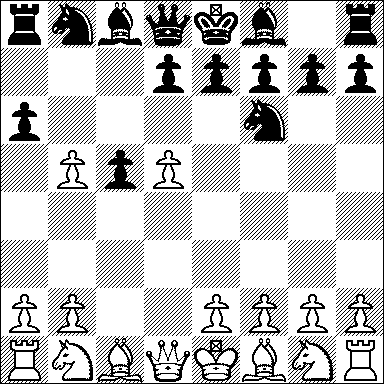
\includegraphics[width=1.40972in,height=1.40972in]{vertopal_109f12be458a423d8f3cc838880eaea2/media/image18.png}

\emph{diagramma 18}

Questa continuazione, nota anche come Gambetto Volga, è del tutto
giocabile ed è l'arma preferita di molti giocatori d'attacco. Il
gambetto ha un sapore del tutto moderno basandosi su un'idea
squisitamente posizionale. Il Nero conquista l'iniziativa sul lato di
Donna facendo pressione sui pedoni a2 e b2 anche grazie al controllo
della diagonale nera a1-h8 e, come se non bastasse, fa pressione sulla
diagonale a6-f1.

\textbf{5.bxa6 ¥xa6 6.¤c3 d6 7.g3 g6 8.¥g2 ¥g7 9.¤f3 0-0 10.0-0 ¤bd7
11.£c2 £a5 12.¦b1 ¦fb8 13.¥d2 ¤b6}

Per finire mettiamo a confronto due modi di giocare lo stesso gambetto.

Le due partite che seguono sono state giocate a distanza di oltre un
secolo, la prima in pieno periodo Romantico, la seconda quando era già
operante la supremazia della scuola sovietica; lo studioso faccia molta
attenzione al diverso spirito che le anima.

Anderssen--Kieseritzky, Londra 1851.

Questa partita, giocata a Londra il 21 giugno 1851, durante una pausa
del primo torneo internazionale della storia degli scacchi, è nota col
nome di ``Immortale''. Essa illustra pe¢fettamente il modo di intendere
gli scacchi all'epoca.

\textbf{1.e4 e5 2.f4 exf4 3.¥c4} in pieno periodo Romantico non si
conoscevano le finezze del gioco posizionale. Ogni mossa o era d'attacco
o era di difesa. In questo ordine di idee si era persa per strada la
concezione di Philidor che i pedoni fossero ``l'anima degli scacchi'';
dal match Bourdonnais-Macdonnell (1834) in poi erano diventati piuttosto
carne da macello. Come è facile immaginare ne scaturivano complicate
baruffe che facevano la gioia degli amanti delle sensazioni forti. Oggi,
si veda la partita successiva, si preferisce la più cauta 3. ¤f3.

\textbf{3... £h4+} all'arrembaggio! Un giocatore moderno opterebbe per
la più semplice (e sana!) 3... ¤f6 oppure per 3... d5.

\textbf{4.¢f1 b5} la mossa preferita da Kieseritsky con la quale si
complica ancora di più il gioco.

\textbf{5.¥xb5 ¤f6 6.¤f3 £h6 7.d3 ch5} minacciando 7... ¤g3+. Si noti in
quanto poco conto siano tenuti i canoni dello sviluppo e si tenda a
creare invece continue minacce con i pochi pezzi già sviluppati.

\textbf{8.ch4 £g5 9.¤f5 c6 10.g4 ¤f6 11.¦g1!} una mossa molto difficile
da trovare. Il Bianco sacrifica l'Alfiere in b5 per guadagnare spazio
sul lato di Re.

\textbf{11... ¤xb5 12.h4 £g6 13.h5 £g5 14.£f3 ¤g8 15.¥xf4 £f6 16.¤c3}
anche un moderno giocatore avrebbe giocato così ma Anderssen la effettua
perché è una mossa d'attacco (minaccia il salto in d5) non per
sviluppare un pezzo.

\textbf{16... ¥c5 17.¤d5 £xb2 18.¥d6!}

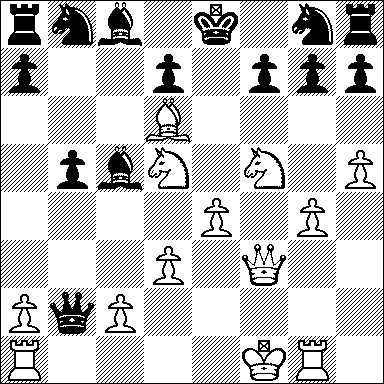
\includegraphics[width=1.40972in,height=1.40972in]{vertopal_109f12be458a423d8f3cc838880eaea2/media/image19.png}

\emph{diagramma 19}

Con la precisione di un ragno il Bianco costruisce la sua tela di matto.
Questa mossa implica il sacrificio delle Torri. Adolf Anderssen fu un
maestro insuperato nell'arte della combinazione.

\textbf{18... ¥xg1 19. e5 £xa1+ 20. ¢e2 ¤a6 21. ¤xg7+ ¢d8 22. £f6+!!}
l'o¢gia di sacrifici culmina con quello di Donna.

\textbf{22... ¤xf6 23.¥e7 matto.}

Spassky--Fischer, Mar del Plata 1960.

Quella che segue è una celebre partita, persa dall'allora diciassettenne
Bobby Fischer contro un Boris Spassky quasi all'apice della carriera. Di
scena è ancora il gambetto di Re, giocato però in versione moderna.
All'attacco frontale sul Re qui si lotta per vantaggi di o¢dine
posizionale.

\textbf{1.e4 e5 2.f4 exf4} invece di accettare il pedone il Nero può
impiantare un controgambetto con 2... d5 (Controgambetto Falkbeer)
3.exd5 e4 4.d3 ¤f6 5.¤bd2 exd3 6.¥xd3 ¤xd5. Poiché il secondo tratto del
Bianco non minaccia realmente il \textbf{§}e5 (a 3.fxe5? seguirebbe 3...
£h4+!) il Nero può anche continuare con una semplice mossa di sviluppo:
2... ¥c5 3.¤f3 d6 4.¤c3 ¤f6 5.¥c4 ¤c3 ecc.

\textbf{3.¤f3 g5 4.h4 g4 5.¤e5 ¤f6 6.d4 d6 7.¤d3 ¤xe4 8.¥xf4 ¥g7 9.¤c3?}
le semplificazioni favoriscono il difendente.

\textbf{9... ¤xc3 10.bxc3 c5 11.¥e2 ¤xd4 12.0-0 ¤c6} quella di Fischer
non è né una mossa di difesa né una di attacco ma una semplice mossa di
sviluppo; ai tempi di Anderssen si sarebbe probabilmente preferito una
mossa difensiva quale 12... h5 ma, come fa notare lo stesso Fischer
nelle note alla partita, dopo 12... h5 13.¥g5 f6 14.¥c1 seguita da
15.¤f4 il lato di Re del Nero è tutto buchi. Nel 1858 questa sensibilità
posizionale era di là da venire.

\textbf{13.¥xg4 0-0 14.¥xc8 ¦xc8 15.£g4 f5 16.£g3 £xc3 17.Tae1 ¢h8
18.¢h1 ¦g8 19.¥xd6 ¥f8 20.¥e5+ ¤xe5 21.£xe5+ ¦g7 22.¦xf5 £xh4+ 23.¢g1
£g4?} occorreva giocare 23... £g3! e dopo 24.£xg3 ¦xg3 il Nero rimane
con un pedone in più.

\textbf{24.¦f2 ¥e7 25.¦e4 £g5 26.£d4 ¦f8?} \emph{``Non vedendo la vera
minaccia del Bianco''} scriverà poi Fischer. \emph{``Io ero preoccupato
per 27.¤e5, senza accorgermi che tale mossa era controbattuta
tranquillamente da 27... ¥c5''.}

\textbf{27.¦e5!} \emph{``Io invece contavo su 27.¤e5? ¦xf2 28.£xf2 ¥c5!
29.£xc5 £xg2 matto.''}

\textbf{27... ¦d8 28.£e4 £h4} \emph{``Sapevo che stavo per perdere un
pezzo, ma ancora non volevo crederci. Dovevo giocare ancora una mossa
per vedere se era proprio vero!''}

\textbf{29.¦f4} il Nero abbandona

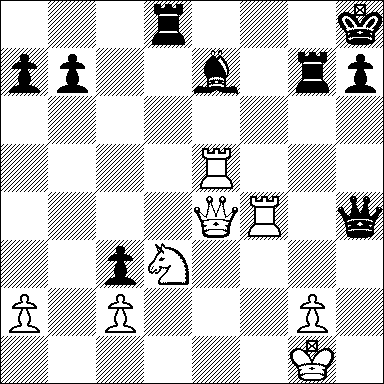
\includegraphics[width=1.40972in,height=1.40972in]{vertopal_109f12be458a423d8f3cc838880eaea2/media/image20.png}

\emph{diagramma 20}

L'Alfiere in e7 cade: 29... £h6 30.¦xe7 ¦xe7 \emph{(30... ¦xd3 31.¦f8+
¦g8 32.£e5+ e poi matto)} 31.£xe7 ¦xd3 32.¦f8+ e matto alla successiva.
Notare come il Bianco abbia conquistato per intero il centro.

\textbf{III -- LA STRUTTURA DEI PEDONI}

\textbf{1. L'indebolimento delle case e il ``buco'' (``foro'',
``hole'')}

Nel commento alla mossa 12 del Nero nella partita Spassky-Fischer, il
campione americano diceva di avere scartato una certa mossa perché
avrebbe condotto a una posizione piena di «buchi». Che cosa intendeva
dire Fischer di preciso? È quel che cercheremo di chiarire in questa
lezione.

Nella posizione iniziale i giocatori controllano ognuno metà scacchiera
e nessun pezzo può installarsi in modo duraturo oltre la terza traversa
perché basta una semplice mossa di pedone per scacciarlo. Se togliessimo
tutti i pedoni dalla scacchiera i pezzi leggeri potrebbero occupare,
senza temere pe¢dite di tempo, anche posizioni avanzate; un eventuale
attacco non li costringerebbe a retrocedere perché potrebbero essere
difesi dagli altri pezzi. Si può dunque affermare che il controllo che
un pedone esercita su una casa è più forte di quello esercitato da un
pezzo. Ne consegue che la funzione delle catene di pedoni è quella di
guadagnare spazio per i pezzi che così possono svilupparsi indisturbati
dietro le linee.

Ovviamente non è tutto oro quel che riluce. Le spinte di pedoni
guadagnano territorio ma a scapito della sicurezza delle retrovie; le
case che si lasciano alle spalle si indeboliscono in quanto non più
difendibili in modo forte (con un pedone). ``Ogni spinta di pedone crea
una debolezza'' sentenziava Steinitz. Il vantaggio di spazio in genere
compensa l'indebolimento delle retrovie ma occorre evitare certe
configurazioni di pedoni che rendono questo indebolimento
particolarmente grave, tanto da diventare, in certi casi, il motivo
dominante della partita. La struttura dei pedoni fa da scudo non solo ai
pezzi ma anche alle case arretrate, le ripara dalle intrusioni
avversarie. Se però nella struttura si producono squarci le case interne
possono indebolirsi a tal punto da diventare buchi.

Ora dovrebbe essere chiaro che cosa si intende per buco: un buco nello
schieramento, poniamo del Bianco, è una casa, nella sua zona di
interesse, non controllabile dai pedoni bianchi; ciò significa che i
pedoni delle colonne adiacenti o sono assenti o sono troppo avanzati.
Chiamiamo zona di interesse di un colore l'insieme delle case occupate,
adiacenti o retrostanti, a pedoni di quel colore. È ovvio che la
presenza del buco sarà ancora più grave se esso è controllato da pedoni
avversari, ma non è detto che un buco renda una casa necessariamente
debole. L'uso della parola è comunque oscillante nei vari autori; da un
lato può estendersi alle case deboli in genere, dall'altro restringersi
al caso sopra ricordato del controllo da parte di un pedone avversario.

Vediamo due esempi:

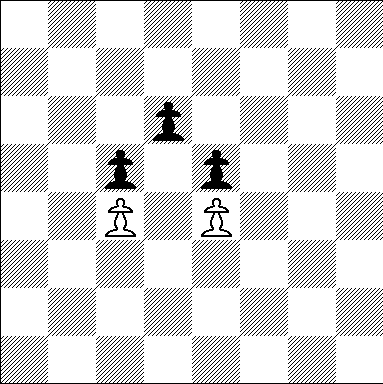
\includegraphics[width=1.40556in,height=1.40903in]{vertopal_109f12be458a423d8f3cc838880eaea2/media/image21.png}

\emph{diagramma 21}

Nello schieramento nero c'è un buco in d5.

\emph{diagramma 22}

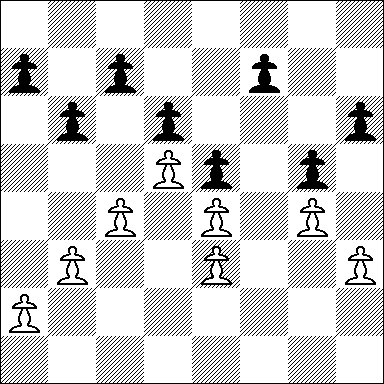
\includegraphics[width=1.40972in,height=1.40972in]{vertopal_109f12be458a423d8f3cc838880eaea2/media/image22.png}

Osserviamo la posizione e facciamo una piccola ricerca di ``buchi''.

Nello schieramento nero se ne contano diversi; in particolare in a6, c6,
f5, f6 e h5. È ovvio che non tutte le case elencate hanno la stessa
importanza strategica. La casa a6 è trascurabile perché decentrata e lo
stesso dicasi per la casa c6 se il Nero ha effettuato l'arrocco corto.
In caso di arrocco lungo sarebbe appetibile perché a ridosso del Re, ma
comunque di difficile sfruttamento se protetta dall'Alfiere in
fianchetto (in b7).

Passiamo a f6: anche senza conoscere la disposizione dei pezzi il piano
di piazzarcene uno in pianta stabile sembra pretenzioso: un Cavallo
potrebbe arrivarci solo attraverso h5, casa che può essere facilmente
guardata con un Cavallo nero posto in g7 o in f6; una Torre, invece,
potrebbe essere scacciata con facilità, per esempio da un Cavallo in d7.

Il buco classico, quello che attira l'attenzione del giocatore esperto,
si trova in f5. Qui si ha una situazione ideale. La casa f5 è per il
Bianco una casa ``forte'', controllata com'è da due pedoni e, per di
più, è facilmente accessibile ai pezzi. Può esserci installato un
Cavallo facendolo passare da g3, casa questa dalla quale i pezzi bianchi
non possono essere in alcun modo intercettati. L'avamposto in f5 può
essere facilmente rafforzato da un secondo Cavallo in g3 e dalle Torri,
eventualmente raddoppiate sulla colonna f.

L'unico foro nello schieramento bianco si trova in h4 ma, poiché
laterale, non è strategicamente di gran valore.

Le conseguenze derivanti anche da un solo buco possono portare alla
sconfitta.

Vediamo che cosa successe nella seguente partita:

Janowsky--Kupchik, L'Avana 1913.

\textbf{1.d4 d5 2.c4 e6 3.¤c3 ¤f6} per evitare continuazioni legate allo
sviluppo del Cavallo in e2 alcuni preferiscono far precedere questa
mossa da 3..¥e7; impedito 3.¥g5, il Bianco non ha modo di ritardare lo
sviluppo del Cavallo di Re.

\textbf{4.¥g5 ¥e7 5.e3 ¤bd7 6.¥d3 £xc4} nella partita di Donna spesso si
assiste a una lotta per il tempo legata alla presa in c4. In molte
varianti il Bianco aspetta che il Nero abbia preso in c4 per uscire
d'Alfiere e il Nero aspetta che il Bianco abbia mosso l'Alfiere per
prendere in c4.

\textbf{7.¥xc4 ¤b6 8. ¥d3 ¤fd5 9.¥xe7 £xe7 10.¤f3 0-0 11.0-0 ¥d7 12.¦c1
c6 13.¤e4}

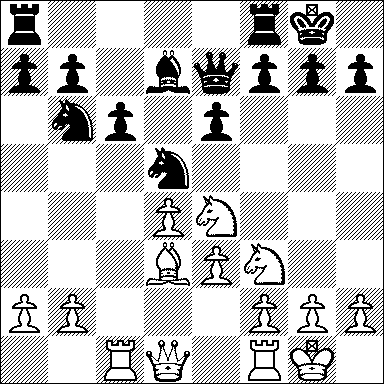
\includegraphics[width=1.40972in,height=1.40972in]{vertopal_109f12be458a423d8f3cc838880eaea2/media/image23.png}

\emph{diagramma 23}

Si è raggiunta una posizione in cui il Bianco è uscito decisamente
meglio dall'apertura. Ha completato in modo sano lo sviluppo e ora può
intraprendere le operazioni di attacco sull'arrocco nero, così decide di
portare un altro pezzo nella zona delle operazioni. Il Nero ha ancora da
completare lo sviluppo: l'¥d7 è accecato dai propri pedoni, il ¤b6 è per
il momento fuori gioco. Intimorito dalle operazioni che il Bianco
minaccia di intraprendere sul lato di Re, il Nero decide di chiudere la
pericolosa diagonale b1-h7 nel modo più drastico:

\textbf{13... f5?} e commette una mossa suicida. In e5 si è infatti
creato un buco che il Bianco non tarderà ad occupare per farne il perno
del proprio attacco.

\textbf{14.¤c5 ¥e8} per portarlo in h5 e dare respiro al povero Alfiere.

\textbf{15.¤e5 ¦b8} così facendo il bianco evita 16... ¥h5 e va nella
casa debole. L'idea del Nero è di giocare ¤d7 per barattare il Cavallo
con quello in e5. Naturalmente il Bianco si guarderebbe bene
dall'acconsentire il cambio; egli è pronto a eliminare un eventuale
Cavallo in d7 col proprio c5. In tal caso otterrebbe anche di riportare
l'Alfiere campo chiaro del Nero nella disgraziata casa d7.

\textbf{16.¦e1 ¦f6} il Nero cerca disperatamente un controgioco sul lato
di Re con ¦h6 e £h4.

\textbf{17.£f3 ¦h6 18.£g3} minaccia 19.¤f7 che attacca
contemporaneamente la ¦h6 con ¤f7 e la ¦b8 con la Donna.

\textbf{18... ¦c8} ammettendo che la quindicesima mossa è stata una
pe¢dita di tempo.

\textbf{19.f3 ¦c7} il Bianco prepara la spinta in e4.

\textbf{20.a3 ¢h8 21.h3 g5 22.e4} ora che tutti i pezzi sono ben
piazzati il Bianco apre il gioco.

\textbf{22... f4} le spinte di pedone hanno creato debolezze nello
schieramento bianco e anche il Nero ha conquistato una casa in
territorio nemico. Questa mossa prepara la discesa di un pezzo.

\textbf{23.£f2 ¤e3} il Cavallo si installa nel buco e3, in posizione
piuttosto fastidiosa.

\textbf{24.¦xe3!} Janowsky non esita a sacrificare la qualità, in cambio
di un solo pedone, pur di eliminare l'avamposto del Nero. Il sacrificio
è più che giustificato perché elimina l'unico pezzo attivo del Nero. Ora
il Bianco ha le mani libere per portare avanti l'attacco. Per qualità si
intende la differenza che intercorre tra il valore della Torre e quella
di un Alfiere o di un Cavallo.

\textbf{24... fxe3 25.£xe3 ¤c8 26.¤g4}

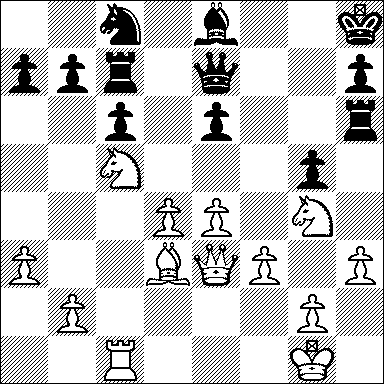
\includegraphics[width=1.40972in,height=1.40972in]{vertopal_109f12be458a423d8f3cc838880eaea2/media/image24.png}

\emph{diagramma 24}

L'idea di questa mossa è di portare il Cavallo in f6. Attaccando la
Torre il Bianco guadagna il tempo necessario per spingere in e5 e
controllare la casa f6. Janowsky rinuncia al buco in e5 per quello, più
avanzato, in f6.

\textbf{26... ¦g6 27.e5 ¦g7 28.¥c4 ¥f7 29.¤f6 ¤b6} questo Cavallo
ballonzola da una casa all'altra senza posa né costrutto.

\textbf{30.cce4} rafforza la presenza del Cavallo in f6.

\textbf{30... h6 31.h4 ¤d5 32.£d2 ¦g6} il Nero è disposto a restituire
la qualità pur di scacciare l'indesiderato intruso.

\textbf{33.hxg5! £f8} la presa 33... hxg5? è sbagliata per via di 34.¢f2
seguita da ¦h1, con facile vittoria.

\textbf{34.f4 ¤e7 35.g4 hxg5 36.fxg5} il Nero abbandona.

Il Bianco minaccia matto in due con 37.£h2+ ¢g7 38.£h7 matto. A 36...
¥g8, che difende in h7, segue 37.£h2+ ¢g7 38.¥xe6~.

Si rifletta come le case e5 prima e f6 dopo siano state per il Nero
delle vere spine nel fianco.

\textbf{2. I pedoni deboli}

Un pedone si dice debole quando non può essere difeso da altri pedoni.
Come è facile immaginare ci sono vari casi di pedoni deboli e vari gradi
di debolezza.

\textbf{a) Il pedone isolato}

Se, nelle colonne adiacenti a quella in cui si trova un pedone, non ce
ne sono altri dello stesso colore (perché catturati o cambiati), quel
pedone si dice ``isolato''.

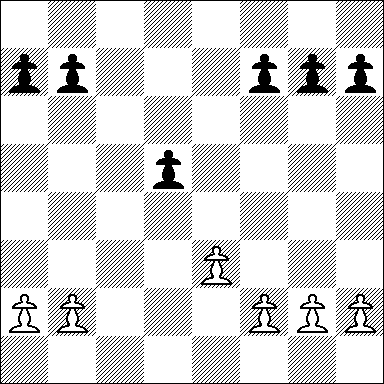
\includegraphics[width=1.40972in,height=1.40972in]{vertopal_109f12be458a423d8f3cc838880eaea2/media/image25.png}\emph{diagramma
25}

Il Pedone in d5 è isolato.

È fuor di dubbio che il pedone isolato sia più debole degli altri ma,
anche se bisogna averne una cura particolare, non sempre è svantaggioso
averne uno.

Può infatti intervenire una compensazione di altra natura, in genere
legata a una maggiore attività dei pezzi leggeri. Per esempio, nella
posizione 25, gli Alfieri neri non trovano ostacoli nei propri pedoni
mentre uno bianco piazzato, poniamo, in c1 avrebbe meno libertà di
azione per via del Pe3. Non stupisca quindi che alcuni sistemi
d'apertura prevedano la formazione di un pedone isolato. Però
attenzione: quando ciò accade il pedone è anche mobile (cioè può essere
spinto ancora). L'ulteriore spinta ne assicura il cambio prima che
diventi debole davvero e può essere usata come ariete contro la catena
di pedoni avversaria. Se, invece, un pedone isolato è bloccato allora la
debolezza è maggiore e può farsi sentire anche in modo pesante durante
la partita.

La debolezza è più grave ancora se, oltre ad essere bloccato, il pedone
isolato si trova su colonna semiaperta (intendendo con questo termine
una colonna sgombra di altri pedoni) perché può essere attaccato anche
con le Torri, eventualmente raddoppiate proprio su quella colonna. Un
simile pedone può facilmente diventare un obiettivo strategico di
primaria importanza.

La formazione di un pedone isolato muta l'indirizzo strategico della
partita: \emph{``Il pedone isolato getta un'ombra sinistra su tutta la
scacchiera''}, disse Tartakower.

Si capisce allora quale strategia adottare appena un pedone isolato si
manifesta nella posizione avversaria. Per prima cosa lo si blocca,
concentrando le forze nella casa successiva a quella in cui il pedone è
posto. Consolidata la conquista della casa di blocco, la si occupa con
un pezzo. Bisogna fare in modo di riprendere, in caso di cambio, con un
altro pezzo e non di pedone. Un'eventuale ripresa col pedone chiuderebbe
la colonna e renderebbe il pedone isolato meno debole. Infine si
mobilitano le forze per farlo cadere.

Vediamo, in due esempi tratti dalle teoria delle aperture, come si opera
per bloccare un pedone isolato.

\emph{Difesa Siciliana:} \textbf{1.e4 c5 2.c3} questa mossa conosce da
qualche anno una certa popolarità, soprattutto perché evita di studiare
le numerose e complicate varianti della Siciliana aperta (2.¤f3 3.d4).

L'obiettivo è di guadagnare spazio al centro, utile per imbastire un
eventuale attacco sull'ala di Re dove è presumibile il Nero arroccherà,
ma ha lo svantaggio di creare un pedone isolato nel proprio
schieramento.

\textbf{2... d5} l'alternativa più comune, 2... ¤f6, evita di portare
subito in gioco la Donna che potrà essere attaccata con pe¢dita di tempo
ma non provoca la formazione di un pedone isolato.

\textbf{3.exd5 £xd5 4.d4 e6} il Nero può rita¢dare il cambio in d4 in
quanto il Bianco non può giocare £xc5 per via di £xd1+.

\textbf{5.¤f3 ¤f6 6.¥d3 ¤xd4 7.¤xd4} il Bianco ha un pedone isolato in
d4. Le prossime mosse del Nero sono finalizzate a consolidare il
controllo della casa d5.

\textbf{7... ¥e7 8.¤c3 £d8 9.0-0 0-0 10.£e2 ¤c6 11.¦d1 ¤b4!} attacca
l'¥d3 e guadagna il tempo necessario per occupare la casa d5.

\textbf{12.¥c4 b6}

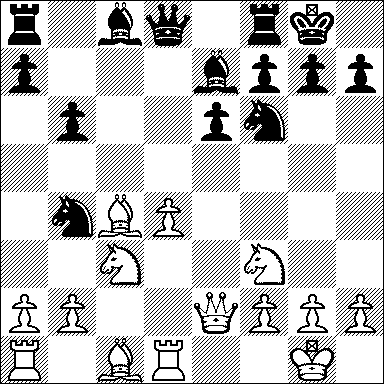
\includegraphics[width=1.40972in,height=1.40972in]{vertopal_109f12be458a423d8f3cc838880eaea2/media/image26.png}

\emph{diagramma 26}

Con l'idea di piazzare l'Alfiere in fianchetto e consolidare
ulteriormente la casa d5. Le mosse successive del Nero saranno dunque
¥b7 e ¤d5, per bloccare in modo definitivo il Pd4 e farne in seguito
oggetto di attacco.

\emph{Difesa Francese:} \textbf{1.e4 e6 2.d4 d5 3.¤d2 c5 4.exd5 exd5
5.¤f3 ¤c6 6.¥b5 ¥d6 7.0-0 ¤ge7 8.£xc5 ¥xc5} in d5 si è creato un pedone
isolato. Dopo quanto si è detto lo scopo delle successive mosse del
Bianco dovrebbe risultare chiaro.

\textbf{9.¤b3 ¥d6 10.c3 ¥g4 11.¤bd4}

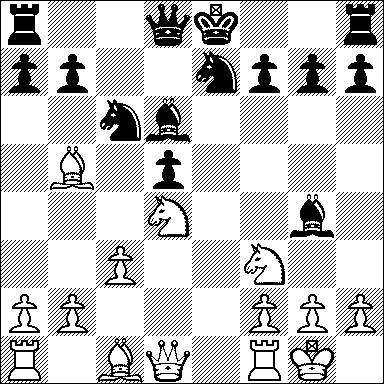
\includegraphics[width=1.40972in,height=1.40972in]{vertopal_109f12be458a423d8f3cc838880eaea2/media/image27.png}

\emph{diagramma 27}

Si noti come in entrambi gli esempi chi blocca abbia superprotetto il
pezzo bloccante in modo da evitare di riprendere con un pedone nel caso
venga cambiato.

\textbf{b) Il pedone arretrato}

Un caso molto simile al pedone isolato, e per il quale valgono molte
delle considerazioni già fatte, è quello del pedone arretrato. Si dice
arretrato un pedone che non può essere difeso da altri pedoni e che si
trova bloccato; il blocco è anche qui più efficace se la casa davanti al
pedone è guardata da almeno un pedone avversario. Anche in questo caso
se il pedone si trova su colonna semiaperta è particolarmente debole.

Il pedone d6 è debole perché arretrato.

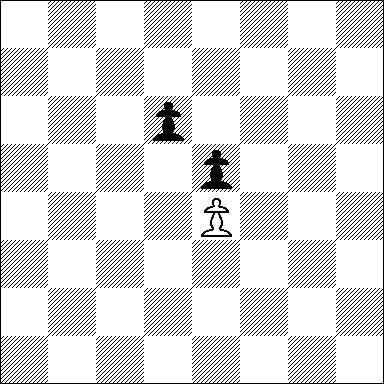
\includegraphics[width=1.40972in,height=1.40972in]{vertopal_109f12be458a423d8f3cc838880eaea2/media/image28.png}\emph{diagramma
28}

Vediamo ora che cosa succede in una variante della difesa Siciliana
venuta in una certa moda nell'ultimo ventennio per merito del GM russo
Evgeni Sveshnikov, da cui prende il nome:

\textbf{1.e4 c5 2.¤f3 ¤c6 3.d4 ¤xd4 4.¤xd4 ¤f6 5.¤c3 e5}

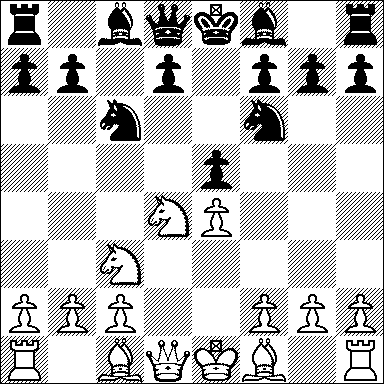
\includegraphics[width=1.40972in,height=1.40972in]{vertopal_109f12be458a423d8f3cc838880eaea2/media/image29.png}\emph{diagramma
29}

Prima degli anni Settanta nessuno giocava così e in tutta la storia
degli scacchi potevano contarsi pochissime partite con questo o¢dine di
mosse. Il motivo risiede nelle debolezze che la mossa e7-e5 provoca
nella struttura dei pedoni neri. Poiché il pedone sulla colonna \emph{c}
non c'è più, la spinta del pedone \emph{e} dà origine inevitabilmente a
debolezze. In caso di spinta di un passo si indebolisce il Pd6 e, se
spinto di due passi, si forma anche un buco in d5. Queste
considerazioni, peraltro giuste, portavano a scartare a priori una mossa
che creava tanti problemi al Nero. Si pensi che nel \emph{``Manuale
teorico pratico delle aperture''} di Giorgio Porreca di 772 pagine
(Milano, Mursia), edito per la prima volta nel 1971 ma ancora in
commercio in una ennesima ristampa, a tale mossa, oggi entrata nel
repertorio anche di grandi maestri di primo piano, è dedicata solo una
piccola nota in cui, peraltro, si dà una continuazione sbagliata.
Sveshnikov fu il primo a rendersi conto che il Nero otteneva vantaggi di
altra natura (grande mobilità dei pezzi leggeri, possibilità di
contrattacco, rimedio drastico contro la spinta di rottura e4-e5) ma la
sua opera fu vista con sufficienza a lungo. Io sono stato uno dei primi
ad adottarla in Italia.

Nel 1977 Sveshnikov venne a giocare un torneo in Italia (Marina Romea).
Per caso alloggiavamo nello stesso albergo e la sera dava spettacolo
vincendo una ``lampo'' dietro l'altra a un maestro russo. Io (allora
semplice Terza Nazionale) rimasi colpito dalla sua variante e decisi di
farne la mia difesa. Vantaggi e svantaggi di questa difficile apertura
sono ben mostrati nella partita che giocai nel Magistrale di Bagni di
Lucca del 1984, contro il maestro americano Stuart Wagman.

Wagman--Leoncini, Bagni di Lucca 1984.

\textbf{1.e4 c5 2.¤f3 ¤c6 3.d4 ¤xd4 4.¤xd4 ¤f6 5.¤c3 e5} oltre che col
nome di Sveshnikov in certi manuali questa variante chiamata anche
Lasker e, di rado, Pilnik o Cebljansky.

\textbf{6. ¤d5 d6} la posizione è caratterizzata da un buco in d5 e un
pedone debole in d6.

\textbf{7.¥g5 a6 8.¤a3 b5 9.¤d5} il Bianco occupa la casa debole.

\textbf{9... ¥e7 10.¥xf6 ¥xf6 11.c3 0-0 12.¤c2} un secondo Cavallo si
prepara a dar man forte al primo via c2 ed e3.

\textbf{12... ¥g5} a 12... ¦b8 il Bianco replica con 13.h4! che prepara
l'attacco sull'arrocco e toglie la casa g5 all'Alfiere.

\textbf{13.a4} l'idea di questa mossa è di distogliere il Pb5 dal
controllo della casa c4 dove il Bianco intende piazzare un Alfiere. Un
Alfiere in c4 fortifica ulteriormente la casa d5 e fa pressione
minacciosamente sulla diagonale a2-g8.

\textbf{13... bxa4 14.¦xa4 a5 15.¥c4 ¦b8} pone sotto pressione il pedone
debole b2.

\textbf{16.¦a2 ¢h8} se il Nero vuole riconquistare la casa d5 deve
minare innanzitutto il Pe4. Questa mossa, che toglie il Re dalla
diagonale a2-g8, prepara la spinta in f7-f5.

\textbf{17.cce3 ¥xe3?!} una mossa di dubbio valore. Il Nero elimina un
controllore di d5 ma il cambio dei pezzi leggeri diminuisce le
possibilità di controgioco.

\textbf{18.¤xe3 ¤e7 19.0-0 f5?} il piano è giusto ma eseguito troppo in
fretta. Il Nero punta a indebolire il Pe4 e ad attaccare sul lato di Re,
ma occorreva far precedere questa mossa da g7-g6 per rispondere a exf5
con gxf5 ed evitare un ulteriore cambio di pezzi leggeri.

\textbf{20.exf5 ¤xf5 21.¤xf5 ¥xf5} questi cambi hanno spuntato le
possibilità di controgioco del Nero e solo un errore del Bianco può
salvarlo dalla sconfitta.

\textbf{22.b3} consolidata la posizione il Bianco è pronto ad iniziare
l'attacco diretto sui pedoni deboli in a5 e d6.

\textbf{22... £d6 23.£d5!} molto ben giocato. Questa mossa mette sotto
osservazione entrambi i pedoni da attaccare e prepara il ra£doppio sulla
colonna con le Torri.

\textbf{23... ¦a8 24.¦d1 ¦fd8} il Nero è costretto a giocare in modo
passivo.

\textbf{25. ¦a1 ¦f8} con l'idea di rispondere con ¥e4 alla presa in a5.
Ormai il Nero è costretto ad arrampicarsi sugli specchi per tenere in
piedi la posizione.

\textbf{26.¦xa5?}

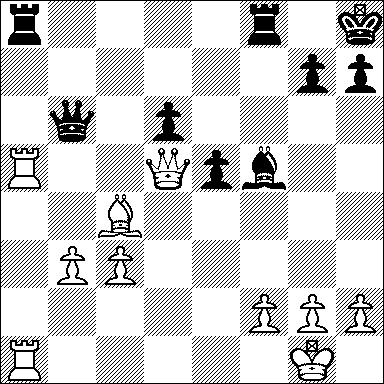
\includegraphics[width=1.40972in,height=1.40972in]{vertopal_109f12be458a423d8f3cc838880eaea2/media/image30.png}

\emph{diagramma 30}

Ecco l'errore! Il Bianco, che fino a questo punto aveva giocato in modo
impeccabile, ora pecca di precipitazione. Wagman aveva visto la replica
del Nero (28... ¥e4) ma aveva preparato una sorprendente mossa di Donna,
purtroppo per lui non sufficiente a contenere il controgioco. Si doveva
far precedere questa presa da 26.£d5! Ora il Nero prende in mano le
redini della partita.

\textbf{26... ¥e4!} minaccia matto in due (27... £xf2+ 28.¢h1 £xg2
matto); se 27.£xe4 ¦xa5.

\textbf{27. £f7!} Wagman aveva riposto le sue speranze in questa mossa
spettacolare; in effetti £f7 salva il materiale ma espone la Donna a
ripetuti attacchi. Con i tempi guadagnati il Nero imbastirà un attacco
micidiale.

\textbf{27... Tac8 28.¦b5} intermedia necessaria per scacciare la Donna
dalla diagonale a7-g1.

\textbf{28... £c6} al solo costo di un pedone il Nero ha conquistato
l'iniziativa e ricolloca i pezzi sulla scacchiera imbastendo minacce su
minacce.

\textbf{29.£e7 ¦ce8} se 29... ¥xg2? 30.¦a7! ¦g8 31.¥xg8 ¦xg8 3 2.¦b8! e
matto alla successiva.

\textbf{30.£g5 ¦f6} la minaccia 31... ¦g6 costringe il Bianco a
indebolire l'arrocco.

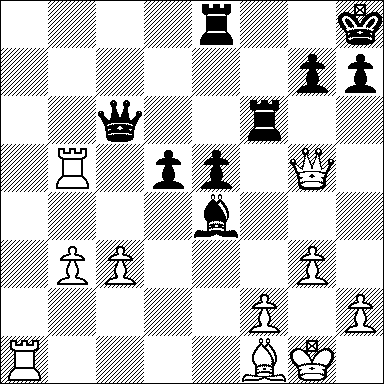
\includegraphics[width=1.40972in,height=1.40972in]{vertopal_109f12be458a423d8f3cc838880eaea2/media/image31.png}\textbf{31.g3
d5 32.¥f1}

\emph{diagramma 31}

\textbf{32... ¦xf2!! 33.¢xf2 ¦f8+ 34.¢g1} a 34. ¢e3 (o 34.¢e1) segue
34... £xc3+.

\textbf{34... £xc3 35.}~il Bianco abbandona. Non c'è modo di parare
tutte e due le minacce 34... £d4+ e 34... £f3 con matto alla seguente.

Da tutto ciò vediamo di trarne qualche insegnamento. Avere ``buchi'' e
pedoni deboli nel proprio schieramento è uno svantaggio che, se non
compensato da altri fattori, conduce alla sconfitta. Quindi occorre
evitare di crearsi debolezze se non si è più che sicuri di ottenere
vantaggi di altra natura.

\textbf{c) Pedoni doppiati (o impedonati)}

Con questo termine si indicano i pedoni del solito colore posti sulla
stessa colonna. La doppiatura dei pedoni è uno svantaggio minimo, di
certo meno grave di un pedone arretrato, anche perché di solito
compensato dall'apertura delle linee.

Gli svantaggi sono intuibili, basti per tutte questa semplice posizione:

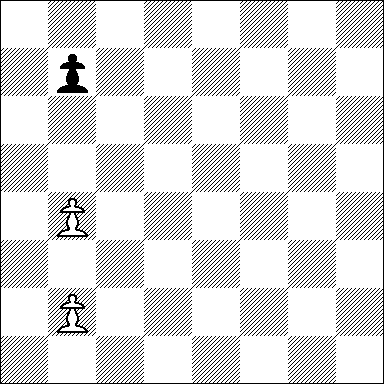
\includegraphics[width=1.40972in,height=1.40972in]{vertopal_109f12be458a423d8f3cc838880eaea2/media/image32.png}

\emph{diagramma 32}

Come si vede il Bianco non ha la possibilità di sfruttare il pedone in
più.

La qualità dello svantaggio di una doppiatura è di diversa portata nelle
diverse fasi della partita e tende ad aumentare a mano a mano che ci si
avvicina al finale. In fase di sviluppo può trovare sufficiente compenso
dall'apertura delle linee; nel centro partita può essere utile avere una
colonna aperta in più ma occorre fare attenzione a che non si trasformi,
con un semplice baratto, in pedone debole; in finale la doppiatura può
equivalere, come nell'esempio, ad avere un pedone in meno.

I pedoni doppiati irrigidiscono le catene di pedoni e facilitano lo
sfondamento avversario; ecco un esempio classico tratto dalla teoria dei
finali:

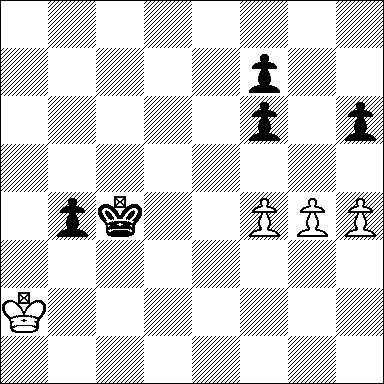
\includegraphics[width=1.40972in,height=1.40972in]{vertopal_109f12be458a423d8f3cc838880eaea2/media/image33.png}\emph{diagramma
33}

Il Bianco vince giocando 1.h5 (1.g5?? fxg5 2.fxg5 h5 e vince il Nero).
seguito da 2.g5.

L'idea di provocare un'impedonatura, e di giungere rapidamente in finale
per sfruttarla a pieno, si ha nella variante di Cambio della Partita
Spagnola:

\textbf{1.e4 e5 2.¤f3 ¤c6 3.¥b5 a6 4.¥xc6 £xc6 5.d4 exd4 6.£xd4 £xd4
7.¤xd4}

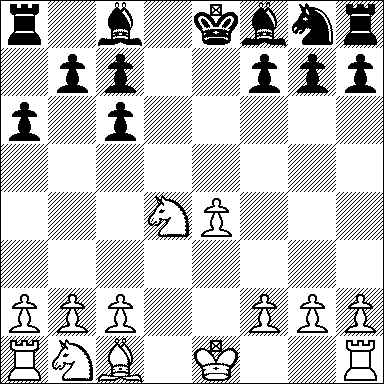
\includegraphics[width=1.40972in,height=1.40972in]{vertopal_109f12be458a423d8f3cc838880eaea2/media/image34.png}\emph{diagramma
34}

Se ora nella scacchiera lasciassimo solo i pedoni il Bianco vincerebbe
facilmente grazie al quattro contro tre sul lato di Re mentre il pedone
in più nero sul lato di Donna, a causa dell'impedonatura, equivale a un
tre contro tre. Al finale di pedoni occorre naturalmente arrivarci; in
questa particolare variante il Nero ha compenso sufficiente grazie alla
coppia degli Alfieri.

\emph{Difesa Francese:} \textbf{1.e4 e6 2.d4 d5 3.¤c3 ¥b4 4.e5 c5 5.a3
¥xc3 6.bxc3}

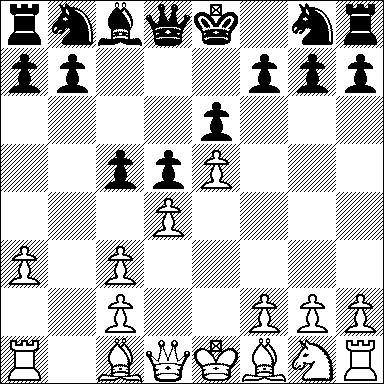
\includegraphics[width=1.40972in,height=1.40972in]{vertopal_109f12be458a423d8f3cc838880eaea2/media/image35.png}

\emph{diagramma 35}

Anche qui l'impedonatura ha, come corrispettivo, la coppia degli
Alfieri. Notare che il pedone in c2 del Bianco può diventare debole e
arretrato dopo il cambio in d4.

\emph{Difesa Caro Kann:} \textbf{1.e4 c6 2.d4 d5 3.¤c3 £xe4 4.¤xe4 ¤f6
5.¤xf6 exf6}

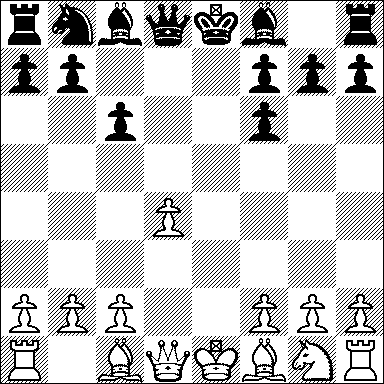
\includegraphics[width=1.40139in,height=1.40139in]{vertopal_109f12be458a423d8f3cc838880eaea2/media/image36.png}

\emph{diagramma 36}

Il Nero ha concesso al Bianco un finale superiore grazie al quattro
contro tre sul lato di Donna. Per compenso ha ottenuto uno sviluppo
scorrevole e un rafforzamento del lato di Re dove intende arroccare. A
differenza delle varianti precedenti il Bianco, però, non si è privato
della coppia degli Alfieri.

I manuali sulle aperture mettono in evidenza che l'idea della difesa
Nimzo Indiana è una sorta di lotta per il controllo delle case centrali.

\textbf{1.d4 ¤f6} questo Cavallo impedisce di piazzare un secondo pedone
al centro e gua¢dare anche la casa d5.

\textbf{2.c4} il Bianco attua un'espansione sul lato di Donna e gua¢da
lo stesso la casa d5.

\textbf{2... e6} stabilisce un secondo controllo su d5 contro uno solo
del Bianco.

\textbf{3.¤c3} pareggia il conto su d5 e minaccia e2-e4.

\textbf{3... ¥b4} inchiodando il ¤c3 annulla gli effetti dell'ultima
mossa bianca.

\textbf{4.a3} la variante Sämisch.

\textbf{4... ¥xc3+ 5.bxc3} nella struttura di pedoni del Bianco è
comparsa una doppiatura di pedoni che può diventare obiettivo del Nero.
Il Nero dovrà prima bloccarlo con la spinta c7-c5 e poi attaccarlo con
¤c6-a5 e ¥c8-a6 (dopo avere ovviamente spinto in b6. Un buon esempio di
questa strategia si ebbe nella partita Geller-Smyslov, giocata
all'Interzonale di Amsterdam nel 1956. Eccone il seguito:

\textbf{5... c5 6.e3 b6 7.¤e2 ¤c6 8.¤g3 0-0 9.¥d3 ¥a6 10.e4 ¤e8 11.¥e3
¤a5 12.£e2 ¦c8 13.d5 £h4 14.0-0 ¤d6} e non ci sono più difese per il
Pc4.

Da questo semplice esempio non si commetta l'errore di credere che la
variante Sämisch sia demolita. Per il pedone doppiato il Nero ha ceduto
la coppia degli Alfieri e si è indebolito il lato di Re. Tanto per dare
un'idea delle possibilità bianche in questa variante si veda la partita
che segue, in cui il lato di Re nero viene letteralmente distrutto.

Lilienthal--Najdorf, Stoccolma 1948, \textbf{(Difesa Nimzo Indiana)}

\textbf{1.d4 ¤f6 2.c4 e6 3.¤c3} per evitare la Nimzo Indiana si può
giocare 3.¤f3 b6 (3... ¥b4+ 4.¥d2) 4.a3 ¥b7 5.¤c3 d5 6.¤xd5 ¤xd5 7.e3
ecc.

\textbf{3... ¥b4 4.a3} le alternative principali, e più comuni di questo
tratto, sono 4.e3 (variante Rubinstein) e 4.£c2 (variante Capablanca).

\textbf{4... ¥xc3+ 5.bxc3 c5 6.e3 ¤c6 7.¥d3 b6} l'occupazione del centro
può essere contrastata con 7... e5 8.¤e2 b6 9.0-0 0-0 10.e4 h6 11.d5 ¤e7
12.f3 ¤g6 13.¥e3 ¥d7 14.£d2 ¦b8 15.a4 b6 16.¤g3 con gioco all'incirca
equivalente, come nella partita Balashov-Lerner, campionato dell'URSS
1985.

\textbf{8.¤e2 0-0 9.e4 ¤e8 10.0-0 d6} è migliore 10... ¥a6 11.f4 f5
12.¤g3 ¤e7 13.exf5 ¤xf5 14.¤xf5 exf5 (Martin-Short, Londra 1985).

\textbf{11.e5!} in considerazione che non è possibile 11.¤xe5?? per
12.¥xh7+ ¢xh7 13.£xd8.

\textbf{11... £xe5 12.£xe5 ¥b7} il vantaggio di spazio del Bianco, che è
ormai pronto a dar l'assalto all'arrocco, non permette al Nero di
sfruttare le debolezze nella struttura di pedoni bianca; anzi, in questa
fase l'impedonatura svolge un ruolo positivo perché permette il
controllo delle case centrali d5 e e5.

\textbf{13.¥f4 f5} un tentativo disperato, ma dopo 13... £c7 il Nero non
ha alcun controgioco da contrapporre all'iniziativa dell'avversario ad
est.

\textbf{14.exf6 e5?} era meglio 14... £xf6 ma al campione a¢gentino era
sfuggita la forza del sacrificio d'Alfiere.

\textbf{15.fxg7 ¦xf4 16.¤xf4 exf4}

\emph{diagramma 37}

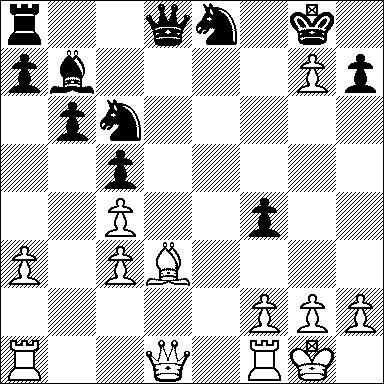
\includegraphics[width=1.4in,height=1.4in]{vertopal_109f12be458a423d8f3cc838880eaea2/media/image37.png}

\textbf{17.¥xh7+!} completa la demolizione dell'arrocco nero. Ora il Re
cade in balìa dei pezzi bianchi.

\textbf{17... ¢xh7 18.£h5+ ¢xg7 19.Tad1 £f6 20.¦d7+ ¢f8 21.¦xb7 ¤d8
22.¦d7 ¤f7 23.£d5 ¦b8 24.¦e1 f3} che altro? A una maggiore resistenza
avrebbe portato 24... ¤e5 25.£xa8 ¤xd7 26.¦e1 £g6 per poi spingere in f3
ma al Bianco è sufficiente collocare la Donna sulla grande diagonale
bianca per evitare il matto.

\textbf{25.¦e3 abbandona}

\begin{enumerate}
\def\labelenumi{\alph{enumi})}
\setcounter{enumi}{3}
\item
  \textbf{Pedoni sospesi}
\end{enumerate}

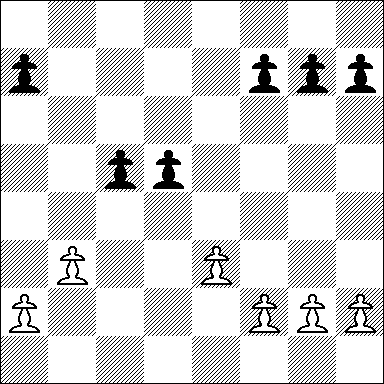
\includegraphics[width=1.40972in,height=1.40972in]{vertopal_109f12be458a423d8f3cc838880eaea2/media/image38.png}\emph{diagramma
38}

I pedoni c5 ed d5 sono deboli perché su colonne aperte. La spinta di uno
di essi provoca il cambio e la debolezza del pedone rimanente. Però,
finché sulla scacchiera sono presenti molti pezzi, i pedoni sospesi
centrali possono rappresentare un punto di forza; la maggiore libertà di
azione di cui godono i pezzi posti dietro ai pedoni passati possono
creare le condizioni per una veloce avanzata verso la promozione di uno
di essi, come accade in questa partita.

Sokolsky--Botvinnik, Leningrado 1938 \textbf{(Difesa Grunfeld)}

\textbf{1.c4 ¤f6 2.¤c3 d5 3.d4 g6 4.¤f3 ¥g7 5.e3 0-0 6.¥e2 e6 7.0-0 b6
8.¤xd5} poiché il Nero si appresta a sviluppare l'Alfiere in fianchetto,
Sokolsky si affretta a chiudere la diagonale a8-h1, ma secondo Botvinnik
era meglio mantenere la tensione al centro con 8.£d3.

\textbf{8... exd5 9.b3 ¥b7 10.¥b2 ¤bd7} per controllare le case e5 e c5.

\textbf{11.£c2 a6 12.Tac1 ¦c8 13.¦fd1 £e7 14.£d1 ¦fd8 15.¥f1 c5 16.£xc5}
commenta Botvinnik: \emph{``Un altro strafalcione posizionale. La
debolezza dei pedoni neri in d5 e c5 non può essere sfruttata, quando è
presente un gran numero di pezzi leggeri e i pedoni sono attaccati dalla
prima traversa. Il Bianco cambia invece il §d4, cedendo l'ultimo
caposaldo centrale; ciò ridà vita all'¥b7''.}

\textbf{16... bxc5}

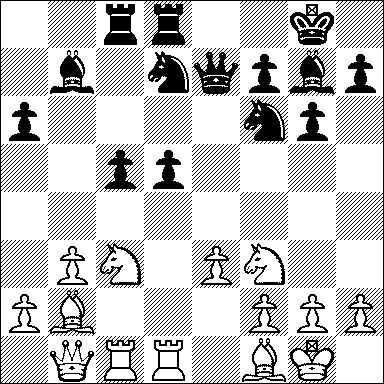
\includegraphics[width=1.40972in,height=1.40972in]{vertopal_109f12be458a423d8f3cc838880eaea2/media/image39.png}

\emph{diagramma 39}

\textbf{17.¤e2 ¥h6} minaccia la spinta in d4.

\textbf{18.¥a3} per rispondere a 18... d4 con 19.¦xd4.

\textbf{18... ¤g4 19.£d3 C£e5 20.¤xe5 £xe5 21.¤g3 £f6 22.ch1 d4 23.£e2
¤e5 24.exd4 ¤xd4}

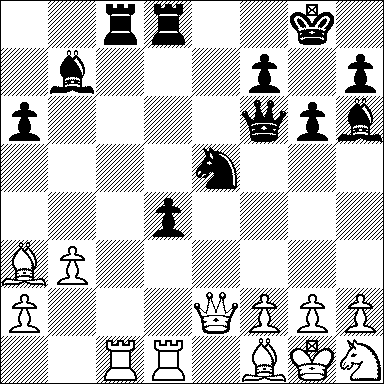
\includegraphics[width=1.40972in,height=1.40972in]{vertopal_109f12be458a423d8f3cc838880eaea2/media/image40.png}

\emph{diagramma 40}

Uno dei due pedoni si è trasformato in pedone passato (o libero),
intendendo con questo termine un pedone la cui marcia non è ostacolata
da pedoni avversari. Se il Bianco avesse modo di bloccarlo, ridisposte
le forze in campo, potrebbe in seguito attaccarlo.

Ma così non è. A causa della forte attività dei pezzi neri il Bianco non
ha modo di bloccarlo ed esso in pochi tratti marcerà trionfalmente a
Donna.

\textbf{25.¦xc8 ¥xc8} la ¦d8 non va distolta dal Pedone libero.

\textbf{26.¦e1 d3! 27.£d1} se 27.£xe5? £xe5 29.¦xe5 d2 e vince.

\textbf{27... ¥g4 28.£a1 d2 29.¦xe5 d1=£ 30.¦e8+ ¦xe8 31.£xf6} finite le
prese il Nero è rimasto con la qualità in più, di certo non compensata
da un unico pedone. Il resto è questione di tecnica.

\textbf{31... ¥e2 32.¤g3 ¥g7 33.£c6 ¥b5 34.£c1 £xc1 35.¥xc1 ¦e1 36.¥e3
¦a1 37.a4 ¥d3 38.f4 ¦b1 39.¢f2 ¥xf1 40.¤xf1 ¦xb3 41.abbandona}

\textbf{3. L'attacco di minoranza}

I cambi possono con facilità creare una asimmetria nella configurazione
pedonale dei giocatori; può crearsi una maggioranza di pedoni su un lato
cui fa da contrappunto quella avversaria sul lato opposto.

La pratica ha dimostrato che se la maggioranza di pedoni è poco mobile
può essere vantaggiosamente attaccata dalla minoranza di pedoni. Quello
che a prima vista può sembrare un paradosso si capisce se si è
familiarizzato con la teoria dei pedoni deboli.

In effetti lo scopo dell'attacco di minoranza è proprio di creare un
pedone debole (sia esso isolato o arretrato) nello schieramento
avversario. Il motivo per cui questo è possibile non è difficile da
capire: cambiando i pedoni ne rimarrà uno, su colonna semiaperta, che
inevitabilmente sarà debole.

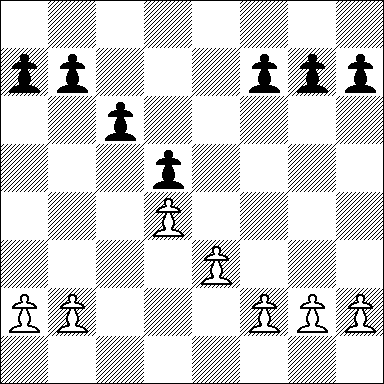
\includegraphics[width=1.40972in,height=1.40972in]{vertopal_109f12be458a423d8f3cc838880eaea2/media/image41.png}\emph{diagramma
41}

Questa è la posizione classica in cui il Bianco può operare un attacco
di minoranza. Sul lato di Donna il Nero ha una maggioranza di quattro
pedoni contro solo tre bianchi, ma la loro mobilità è ridotta. Infatti,
la spinta in c5 isolerebbe il Pd5 dopo d4xc5; la spinta in b6 renderebbe
più debole quello in c6. In queste condizioni un eventuale assalto del
Bianco è giustificato. L'attacco avviene spingendo a fondo i pedoni
``a'' e ``b''. Giunto in b5 il pedone minaccia la presa in c6 perché
dopo b7xc6 nella struttura del Nero si forma un pedone arretrato (c6).
D'altra parte, se il Nero gioca d'anticipo c6xb5, dopo a4xb5 il Bianco
può puntare i suoi cannoni sul pedone ``a''. Infine, come abbiamo già
detto, non serve nemmeno la spinta c6-c5 perché dopo d4xc5 il pedone d5
rimane isolato.

Prima di esaminare l'attacco di minoranza nella pratica, vediamo al
solito, alcune aperture che creano le condizioni per tale strategia.

\emph{diagramma 42}

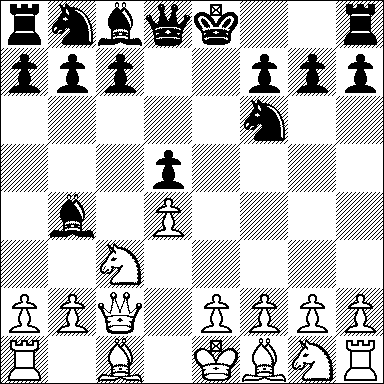
\includegraphics[width=1.40972in,height=1.40972in]{vertopal_109f12be458a423d8f3cc838880eaea2/media/image42.png}

\emph{Difesa Nimzo Indiana:} \textbf{1.d4 ¤f6 2.c4 e6 3.¤c3 ¥b4 4.£c2 d5
5.¤xd5 exd5}

\emph{Difesa Gruenfeld:} \textbf{1.d4 ¤f6 2.c4 g6 3.¤c3 d5 4.¤f3 ¥g7
5.¥g5 ¤e4 6.¤xd5 ¤xg5 7.¤xg5 e6 8.¤f3 exd5}

\emph{diagramma 43}

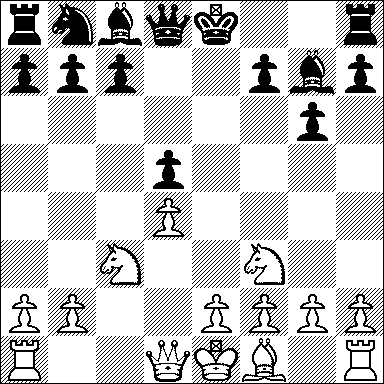
\includegraphics[width=1.40972in,height=1.40972in]{vertopal_109f12be458a423d8f3cc838880eaea2/media/image43.png}

\emph{Difesa Caro Kann:} \textbf{1.e4 c6 2.d4 d5 3.exd5 ¤xd5 4.¥d3 ¤c6
5.c3}

\emph{diagramma 44}

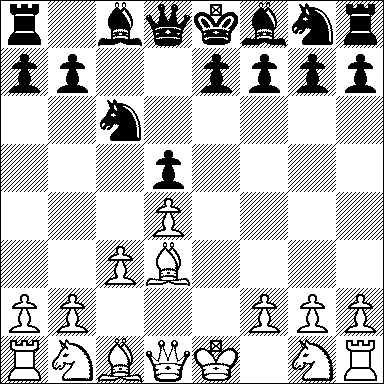
\includegraphics[width=1.40972in,height=1.40972in]{vertopal_109f12be458a423d8f3cc838880eaea2/media/image44.png}

\emph{Difesa Cambridge Springs:} \textbf{1.d4 d5 2.c4 e6 3.¤c3 ¤f6 4.¥g5
c6 5.e3 ¤bd7 6.¤f3 £a5 7.¤xd5 exd5}

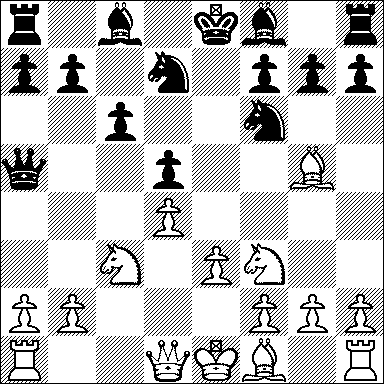
\includegraphics[width=1.40972in,height=1.40972in]{vertopal_109f12be458a423d8f3cc838880eaea2/media/image45.png}\emph{diagramma
45}

Il caso tipico, quello in cui l'attacco di minoranza avviene quasi di
norma, si ha nella Variante di Cambio del Gambetto di Donna:

\textbf{1.d4 d5 2.c4 e6 3.¤c3 ¤f6 4.¥g5 ¥e7 5.¤xd5 exd5 6.¤f3 c6}

\emph{diagramma 46}

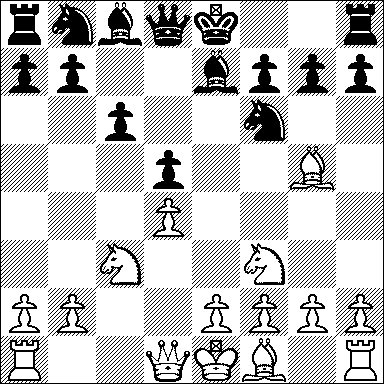
\includegraphics[width=1.40972in,height=1.40972in]{vertopal_109f12be458a423d8f3cc838880eaea2/media/image46.png}

Data la semplicità, e linearità di esecuzione, l'attacco di minoranza
può essere molto pericoloso anche in mano a un giocatore non
espertissimo.

Le reazioni possibili sono, in sostanza, due:

\emph{a)} contrattaccare sul lato opposto a quello in cui si sviluppa
l'attacco di minoranza;

\emph{b)} contrastarlo in modo diretto sullo stesso lato.

\textbf{a) Il contrattacco a un attacco di minoranza}

Abbiamo visto che nell'attacco di minoranza si spingono a fondo i propri
pedoni dopo avere ovviamente arroccato sull'altro lato della scacchiera.
La reazione energica sull'ala opposta avrà quindi le caratteristiche di
un assalto all'arrocco.

La partita che segue ne è un esempio e riassume bene quanto finora
spiegato.

Averbach--Konstantinopolsky, Mosca 1966 \textbf{(Gambetto di Donna
Rifiutato)}

\textbf{1.d4 d5 2.c4} si potrebbe discutere se a rigor di termini questo
debba essere considerato un gambetto. Dopo 2... £xc4 il vantaggio di
materiale è solo temporaneo non avendo modo il Nero di difendere il Pc4
a oltranza. Per esempio: 3.e3 b5 4.a4 c6 5. axb5 ¤xb5 6.£f3 con attacco
imparabile alla Torre in a8.

\textbf{2... c6 3.¤f3 e6 4.¤xd5 exd5 5.¤c3 ¤f6 6.¥g5 ¥e7 7.£c2 ¤bd7 8.e3
0-0 9.¥d3 ¦e8 10.0-0 ¤f8 11.Tab1}

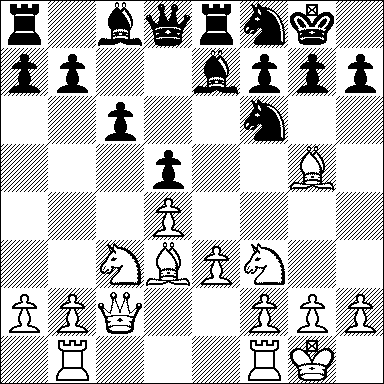
\includegraphics[width=1.40972in,height=1.40972in]{vertopal_109f12be458a423d8f3cc838880eaea2/media/image47.png}

\emph{diagramma 47}

Finita la fase di sviluppo il Bianco prepara la spinta in b4. Ha inizio
l'attacco di minoranza. A mio parere il Bianco poteva arrivare alla
spinta in b4 un tempo prima giocando 11.¥xf6! (distoglie l'¥e7 dal
controllo di b4) con la seguente continuazione: 11... ¥xf6 12. b4

\textbf{11... ¤e4 12.¥xe7 £xe7 13. b4 a6 14.a4 ¤g6} alle spinte dei
pedoni sul lato di Donna il Nero reagisce imbastendo un contrattacco
sull'ala di Re.

\textbf{15.b5 axb5 16.axb5 ¥g4 17.¥xe4!}

\emph{diagramma 48}

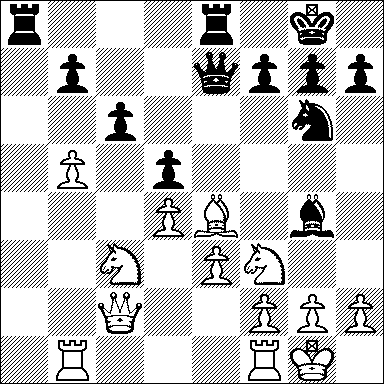
\includegraphics[width=1.40972in,height=1.40972in]{vertopal_109f12be458a423d8f3cc838880eaea2/media/image48.png}

In una partita giocata a Kiev nel 1954, in occasione del XXI Campionato
sovietico, Taimanov, contro Nezmetdinov, giocò meno correttamente 17.
¤d2? ma dopo 17... ¤xd2, 18.£xd2 ch4!, (minaccia 19... ¤f3+ o anche
19... ¥h3) l'attacco del Nero arriva prima. Per esempio: 19.¥e2 ¥h3!,
20.gxh3 £g5+, 21.¥g4 ¤f3+. Taimanov fu allora costretto a ripiegare su
19.f3 £xe3+ 20.£xe3 ¦xe3, 21.fxg4 ¦xd3, 22.bxc6 bxc6 (non si può 22...
¦xc3? per 23.¤xb7 ¦b8, 24.¦bc1 ¦c4, 25.¦xc4 £xc4, 26.¦a1), 23.¤e2 ¦d2,
24.¦f2 h6, 25.¦bf1 ¤g6, e riuscì a salvare questa partita solo grazie a
successivi errori del Nero.

\textbf{17... £xe4 18.¤d2! ¥f5} una mossa dubbia. Forse è migliore 18...
f5.

\textbf{19.bxc6 bxc6} lo scopo dell'attacco di minoranza è raggiunto: il
c6 pedone è isolato.

\textbf{20.¤e2 ch4} il Bianco rafforza il lato di Re e attacca il Pc6.

\textbf{21.¤g3 ¥g6}

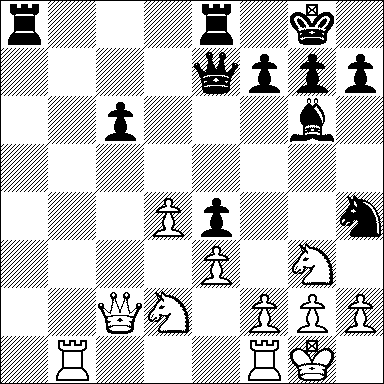
\includegraphics[width=1.40972in,height=1.40972in]{vertopal_109f12be458a423d8f3cc838880eaea2/media/image49.png}\emph{diagramma
49}

Si imponeva 21... Tac8. Konstantinopolsky temeva 22. f3 senza accorgersi
della forte risposta 22... £g5. Ora il Pc6 cade senza sufficiente
compenso.

\textbf{22.£xc6 Tac8 23.£d5 f5 24.¦fc1 ¦xc1+ 25.¦xc1 f4 26.exf4 e3
27.£d3+ ¥f7 28.£xe3 £d7 29.C£e4 ¥g6 30.f5 ¤xf5 31.¤xf5 ¦xe4 32.¤d6 ¦xe3
33.fxe3 £d7 34.¦c8+ £xc8 35.¤xc8} il Nero abbandona.

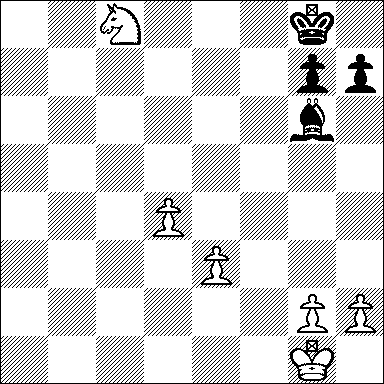
\includegraphics[width=1.40972in,height=1.40972in]{vertopal_109f12be458a423d8f3cc838880eaea2/media/image50.png}

\emph{diagramma 50}

La strategia del Bianco ha trionfato!

\textbf{b) contrastare l'attacco sullo stesso lato.}

Il modo più drastico di rispondere a un attacco di minoranza è, dopo
b2-b4, di giocare b7-b5 e piazzare un Cavallo in c4. La casa debole in
c5 trova il suo corrispettivo in quella c4 mentre il pedone c6 debole
non è facilmente sfruttabile dal Bianco dopo che il Nero, piazzato un
Cavallo in c4, ha chiuso la colonna a possibili attacchi di pezzi
pesanti. Si capisce pertanto come la mossa b7-b5 sia strettamente
connessa con ¤c4; se quest'ultima non fosse possibile la spinta del
pedone in b5 si rivelerebbe un gravissimo indebolimento. Attenzione
però: questa strategia può essere adottata solo se al Bianco è
interdetta la mossa b2-b3 che scaccerebbe il ¤c4 e renderebbe debole il
pedone in c6.

Mambrini--Leoncini, Imperia 1992 \textbf{(Gambetto di Donna Rifiutato)}

\textbf{1.d4 d5 2.c4 e6 3.¤c3 ¤f6 4.¥g5 ¥e7 5.¤xd5} il Bianco svela i
suoi piani. Per confermare la norma di Maestro era importante che
vincessi questa partita. Dover entrare in una variante in cui la
strategia del Bianco è semplice e valida per molte mosse, non mi fece
per niente piacere.

\textbf{5... exd5 6.£c2 g6!} nella partita di Donna lo sviluppo
dell'Alfiere campochiaro è un problema non irrilevante per il Nero. Con
la minaccia ¥f5 il Nero pone le basi per cambiarlo con quello buono del
Bianco. Il Bianco può evitare questa variante con l'adozione una diversa
successione di mosse; per esempio giocando 6.e3, in modo da replicare
alla spinta in g6 con 7.¥d3, mossa che impedisce 7... ¥f5, cui
seguirebbe 8.¥xf5! gxf5 e il Nero dove arrocca?

\textbf{7.e3 ¥f5 8.¥d3 ¥xd3} se il Bianco vuole evitare il cambio degli
Alfieri su casa chiara può giocare 8.£d3.

\textbf{9.£xd3 ¤bd7} una mossa importante. In caso di cambio in f6
occorre riprendere di Cavallo per non distogliere l'¥e7 dal controllo di
b4 (cfr. nota alla undicesima mossa bianca nella partita precedente).

\textbf{10.¤f3 0-0 11.0-0 c6 12. ¦ab1}

\emph{diagramma 51}

\includegraphics[width=1.40972in,height=1.40972in]{vertopal_109f12be458a423d8f3cc838880eaea2/media/image51.png}Eccoci
giunti al bivio: attaccare sul lato di Re o contrastare palmo a palmo
l'espansione del Bianco sull'ala di Donna? In questa partita optai per
la seconda strategia per ragioni puramente psicologiche. Avendo più
punti Elo del mio avversario volevo evitare che il suo compito fosse
facilitato dal dover eseguire un piano semplice.

Opporsi all'espansione significava costringerlo a una battaglia dalla
strategia non scontata dove speravo di far valere la mia presunta
(quanto è attendibile il punteggio Elo?) maggiore forza.

\textbf{12... a5 13.a3?} il Bianco deve arrivare alla spinta in b4 ma
dopo questa mossa tale spinta non è più possibile! Si dovevano muovere i
pedoni in un o¢dine diverso: b3, a3 e b4. La spinta in a5 è utile a
ritardare l'espansione bianca.

\textbf{13... a4!} ora a una eventuale spinta del pedone b, il Nero
cambia il pedone e il Bianco rimane con un pedone arretrato in a3.

\textbf{14.£c2 b5} solo ora che il Bianco non ha più modo di gua¢dare
con un pedone la casa c4 questa mossa può essere giocata.

\textbf{15.¥xf6 ¥xf6} il Nero può riprendere tranquillamente d'Alfiere
non essendo più necessario controllare la casa b4. Inoltre il Cavallo in
d7 è destinato ad andare in c4 (via b6).

\textbf{16.¤a2 ¦c8 17.¤b4} siccome in c6 c'è un pedone debole, il Bianco
ripiazza i pezzi per attaccarlo. Ma, come si vedrà, l'idea è
irrealizzabile. La casa ideale del Cavallo bianco è piuttosto in c5.

\textbf{17... ¤b6 18.b3?}

\emph{diagramma 52}

\includegraphics[width=1.40972in,height=1.40972in]{vertopal_109f12be458a423d8f3cc838880eaea2/media/image52.png}

La mossa perdente! Il Bianco si accorge di non poter prendere in c6:
18.¤xc6? £d7!, 19. ¦fc1 ¤c4 e, dopo la ritirata del Cavallo bianco,
20... ¤xe3. Inoltre l'attacco di minoranza è stato frustrato sul
nascere, di più, è stato il Nero a guadagnare terreno sul lato di Donna.
In simili occasioni è facile sbagliare.

\textbf{18... axb3} il Nero ha finalmente un obiettivo concreto: il Pa3!

\textbf{19.£xb3 £d6 20.¦fc1 ¦c7} il Nero intende raddoppiare le Torri
sulla colonna ``a'' ma la ¦c8 per il momento non può essere distolta
dalla difesa del \textbf{§}c6, quindi lascia libero il passaggio verso
la colonna ``a'' alla ¦f8 e prepara il raddoppio in a7.

\textbf{21.¤a6 ¦a7 22.£d4 ¦d8 23.¤c5 T£a8 24.¤e4 £e6 25.¤c5} il Cavallo
si piazza nel buco in c5 ma, tutto sommato, a questo punto era meglio
cambiare in f6. Il mio avversario sperava forse che acconsentissi alla
patta per ripetizione di posizione.

\textbf{25... £e8! 26.¦a1 ¥e7 27.¤e5?} una mossa ottimista. Il Bianco
non sembra essersi reso conto che è giunto il momento di difendersi con
i denti. Sarebbe stato meglio 27.¤d2 per essere pronti a cambiare il
Cavallo nero appena spicca il salto in c4.

\textbf{27... f6 28. Ced3 ¤c4}

\includegraphics[width=1.40972in,height=1.40972in]{vertopal_109f12be458a423d8f3cc838880eaea2/media/image53.png}

\emph{diagramma 53}

Finalmente il Cavallo si installa nella casa c4 e con effetti
dirompenti. Il terzo attacco al Pa3 è senza rimedio.

\textbf{29.¦xc4?} vistosi perduto il Bianco sacrifica la qualità
sperando in una boccata d'ossigeno. In realtà questa mossa affretta la
fine.

\textbf{29... bxc4 30.¤f4 ¦b8 31.£c3 ¥xc5 32.£xc5 £e5} in vantaggio di
materiale il Nero può cambiare tranquillamente i pezzi e, in caso di
ritirata della Donna bianca, questa mossa guadagna comunque spazio.

\textbf{33.£c1 Tab7} dopo questa mossa il Bianco non ha più difese. La
conclusione è rapida.

\textbf{34.f3 £xa1! 35.£xa1 ¦b1+ 36.£xb1 ¦xb1+ 37.¢f2 c3}

\includegraphics[width=1.40972in,height=1.40972in]{vertopal_109f12be458a423d8f3cc838880eaea2/media/image54.png}

\emph{diagramma 54}

Il Pedone ``c'' marcia trionfalmente a promozione perciò il Bianco
abbandona.

\textbf{4. I pedoni forti}

\textbf{a) Il pedone passato isolato}

Per pedone passato (o libero) si intende un pedone che, davanti a sé, ha
sgombre di pedoni avversari la colonna in cui si trova e quelle
adiacenti.

La forza di un pedone libero ma isolato dipende da alcuni fattori:

\emph{a)} La sua forza aumenta più è avanzato. Se si trova nella seconda
o terza traversa, tra l'importanza strategica di essere libero e la
debolezza di essere isolato prevalgono in genere i fattori di debolezza.
L'avversario infatti ha di norma tutto il tempo e lo spazio per
preparare una casa di blocco ed attaccarlo in forze.

Se invece si trova ben difeso oltre la quarta traversa allora prevalgono
i motivi che ne fanno una forza. Oltre a rappresentare una minaccia
costante di promozione, può essere spinto, ed eventualmente sacrificato,
per sgomberare una casa o aprire una colonna. È vero che un pedone
libero ma isolato lega anche i pezzi alla sua difesa ma il vantaggio di
spazio e la maggiore libertà di manovra sono in genere un buon compenso.

\emph{b)} Il valore della sua forza aumenta in rapporto alla sua
mobilità. Per questa ragione il difendente deve bloccarne l'avanzata. Il
bloccatore più adatto sono i pezzi minori, perché non scacciabili con un
semplice attacco.

\emph{c)} La sua forza aumenta a mano a mano che ci si avvicina al
finale di partita. In finale la sua forza è massima quando è distante
dal resto dei pedoni.

\emph{diagramma 55}

\includegraphics[width=1.40972in,height=1.40972in]{vertopal_109f12be458a423d8f3cc838880eaea2/media/image55.png}

Entrambi i giocatori hanno un pedone libero ma quello del Bianco vale di
più perché è lontano.

La strategia per vincere è semplice. Il Bianco spingerà il pedone ``a''
ed il Re Nero sarà costretto ad andare a prenderlo; in questo modo però
si allontanerà dai propri pedoni che saranno catturati facilmente dal
Bianco.

\textbf{1.a4 ¢c4} distratto dall'azione diversiva il cane da guardia
lascia sole le pecorelle che divengono facili prede del lupo bianco.

\textbf{2.a5 ¢c5 3.¢d3 ¢b5 4.¢xd4 ¢xa5 5.¢e5} il Bianco vince.

\textbf{b) Il pedone passato sostenuto}

Un pedone libero, e sostenuto da altri pedoni, è un obiettivo
importante. La sua forza d'attacco è ancora maggiore di quello isolato
perché non abbisogna di pezzi alla sua difesa, pezzi che così possono
essere usati in altri compiti, per essere sostenuto. Anche in questo
caso la sua forza aumenta nel finale ed è massima in quello di soli
pedoni perché limita drasticamente l'azione del Re avversario inchiodato
al suo controllo.

\emph{diagramma 56}

\includegraphics[width=1.40972in,height=1.40972in]{vertopal_109f12be458a423d8f3cc838880eaea2/media/image56.png}

Il Bianco vince facilmente andando a prendere con il Re i pedoni
avversari.

Il Re Nero, non potendo uscire dal quadrato a5-a8-d5-d8, non ha alcun
modo di contrastare questa semplice manovra.

Abbiamo già avuto modo di vedere in azione la terribile forza di un
pedone passato (cfr. partita Sokolsky--Botvinnik dopo la
24\textsuperscript{a} mossa del Nero e anche la Mambrini--Leoncini dopo
la 29\textsuperscript{a} mossa).

Vediamo ancora qualche esempio.ù

\emph{diagramma 57}

\includegraphics[width=1.40972in,height=1.40972in]{vertopal_109f12be458a423d8f3cc838880eaea2/media/image57.png}

Questa posizione si verificò nella partita giocata nel torneo A.V.R.O.
del 1938 tra Botvinnik e Capablanca.

Il Nero ha un pedone in più e la spinta del pedone libero ``a'' è un
piano semplice e vincente; il compenso del Bianco si basa sul
\textbf{§}e6 passato e avanzato. Il Nero lo ha bloccato con la Donna e
si appresta a far valere il pedone in più; purtroppo per lui la Donna
non è un bloccatore ideale perché al minimo attacco è costretta a
spostarsi. In apparenza comunque non si vede quale pezzo possa darle
fastidio.

\textbf{30.¥a3!! £xa3} la mossa del bianco è un fulmine a ciel sereno!

\textbf{31.ch5+!} scardina la posizione del Nero e confida nella forza
congiunta di Donna e pedone passato.

\textbf{31... gxh5 32.£g5+ ¢f8 33.£xf6+ ¢g8 34.e7} decisiva! Al Nero non
rimane che un inutile caccia allo scacco perpetuo.

\textbf{34... £c1+ 35.¢f2 £c2+ 36.¢g3 £d3+ 37.¢h4 £e4+ 38.¢xh5 £e2+
39.¢h4 £e4+ 40.g4 £e1+ 41.¢h5} non ci sono più scacchi pertanto il Nero
abbandona.

Il diagramma 58 riproduce la posizione prodottasi dopo la
ventiquattresima mossa del Nero della partita Bernstein--Capablanca del
torneo di Hastings del 1922.

\includegraphics[width=1.40972in,height=1.40972in]{vertopal_109f12be458a423d8f3cc838880eaea2/media/image58.png}\emph{diagramma
58}

Il pedone passato in c3 ha concentrato su di sé tutti i pezzi della
scacchiera. La sua presenza limita alquanto le possibilità del Bianco,
costretto a muoversi in spazi ristretti.

Il Bianco ha realizzato un blocco in c2 ma il bloccatore è un pezzo
pesante e quindi sarà costretto a muoversi in caso di un attacco di
Cavallo. In effetti, un eventuale raddoppio delle Torri nere sulla
colonna ``c'' consentirebbe al Nero di spostare il Cavallo che potrebbe
ripiazzarsi più convenientemente in b4 (o a3) per scacciare la Torre
dalla casa c2.

Il Bianco ha in animo di impedire il raddoppio e gioca:

\textbf{24.¤b3 ¦c6 25.¤d4} dove mettere la Torre? La casa c4 è
controllata dalla Donna; se la Torre torna in c5 il Bianco gioca il
Cavallo in b3 e ripete la posizione; a 25... ¦c7 segue invece 26. ¤b5 ed
il pedone c3 cade. Il Nero deve quindi andare in c8 e rita¢dare di varie
mosse l'attacco alla casa c2. Nel frattempo il Bianco può prendere
provvedimenti. Questo almeno è quanto doveva pensare Bernstein ma lo
attendeva una sorpresa:

\textbf{25... ¦c7} Bernstein, non vedendo il sottile tranello basato
sulla debolezza della prima traversa, deve aver pensato a un errore del
Campione del Mondo e, come preventivato, decide di guadagnare il pedone.

\textbf{26.¤b5 ¦c5 27.¤xc3 ¤xc3 28.¦xc3 ¦xc3 29.¦xc3 £d2!!} ecco la
bellissima mossa che Capablanca aveva preparato. Dopo questa mossa non
ci sono più difese. A 30.£xb2 segue 30... ¦d1 matto; se invece 30.¦c2
£d1+ 31.£f1 £xc2; se, infine, 30.£e1 £xc3! 31.£xc3 ¦d1 e matto alla
seguente.

\textbf{30.} il Bianco abbandona.

\includegraphics[width=1.40972in,height=1.40972in]{vertopal_109f12be458a423d8f3cc838880eaea2/media/image59.png}

\emph{diagramma 59}

Per finire seguiamo le evoluzioni dei pezzi in una partita in cui
prevale la tecnica difensiva. Lo studio attento di questa istruttiva
partita dice molto su come contrastare la forza di un pedone passato.

Leonhardt--Nimzowitsch, San Sebastian 1912 \textbf{(Difesa Philidor)}

\textbf{1.e4 e5 2.¤f3 d6 3.d4 ¤f6 4.¤c3 exd4} forse è migliore non
cedere il centro e giocare 4... ¤bd7 5.¥c4 ¥e7 6.0-0 0-0 7.a4 c6.
Nimzowitsch fu un grande sperimentatore di linee difensive portando
molte innovazioni nel campo della teoria delle aperture e rivisitando in
chiave moderna, come fa in questa partita, difese considerate inferiori.

\textbf{5.¤xd4} una linea più aggressiva si ha con 5.£xd4 e se 5... ¤c6
allora 6.¥b5! ¥d7 7.¥xc6 e la coppia degli Alfieri trova compenso dal
vantaggio del Bianco al centro.

\textbf{5... ¥e7 6.¥e2 0-0 7.0-0 ¤c6 8.¤xc6 bxc6} Nimzowitsch commenta:
\emph{``Il cambio crea vantaggi per entrambi: il Nero ottiene una massa
di pedoni centrali più compatta (che impedisce l'occupazione della casa
d'avamposto d5 con l'eventuale ¤d5), ma il §a7 è isolato e anche c5 può
diventare debole, come nel testo.''}

\textbf{9.b3 d5 10.e5 ¤e8 11.f4 f5} la minaccia f4-f5 costringe il Nero
a questa spinta di pedone che dona al Bianco un pedone passato e
sostenuto in e5.

\textbf{12.¥e3 g6}

\includegraphics[width=1.40972in,height=1.40972in]{vertopal_109f12be458a423d8f3cc838880eaea2/media/image60.png}\emph{diagramma
60}

Come sappiamo il Nero deve bloccare il pedone passato nella casa e6 e il
modo migliore per farlo è con un pezzo leggero. I pezzi leggeri che
possono andare in e6 sono solo due l'¥c8 e il ¤e8, ma è facile vedere
che un ¥e6 svolgerebbe un ruolo del tutto passivo quindi è ovvio che
Nimzowitsch intenda portarci il Cavallo. Oltre a bloccare il pedone
passato, un Cavallo in e6 prepara le importanti spinte di rottura in d4
e g5.

Questa mossa si rende dunque necessaria per preparare la strada al
Cavallo che giungerà in e6 via g7.

\textbf{13.¤a4 ¤g7 14.£d2 £d7 15.£a5} oltre a fare pressione sul lato di
Donna questa mossa vuole impedire la manovra nera a5-¥a6 col conseguente
cambio degli Alfieri su casa chiara.

\textbf{15... ¤e6 16.Tad1 ¦d8 17.¤c5?} una mossa ``naturale'' ma in
realtà un errore strategico. L'idea di occupare la casa c5 è giusta ma
il Bianco doveva portarci l'Alfiere, e solo dopo aver cambiato l'Alfiere
camposcuro, piazzarci il Cavallo. È importante rimuovere il bloccatore
in e6 e solo un Cavallo poteva riuscirci.

\textbf{17... ¥xc5} eliminato il Cavallo c5 il Bianco non ha più modo di
scacciare il bloccatore e di far valere, nel mediogioco, il pedone
passato. Ora l'iniziativa passa nelle mani del Nero.

\textbf{18.¥xc5 ¥b7 19.¦f3 ¢f7 20.¦h3 ¢g7 21.¦f1 ¦e8 22.¦hf3 Tad8 23.¦d1
a6} 23... £xa7? perde la Donna dopo 23... ¦a8 24.£xb7 Teb8.

\textbf{24.b4 ¢h8 25.£a3 ¦g8 26.£c3 ¦g7 27.¢h1 T£g8 28.¥e3 c5 29.¦g3}
secondo Schlechter era migliore 29.bxc5, col probabile seguito 29... d4
30.¦xd4! ¤xd4 31.¥xd4 ¥xf3 32.¥xf3 con due Alfieri e due pedoni per le
Torri.

\textbf{29... d4 30.£a3 g5 31.¥c4 gxf4 32.¥xe6}

\emph{diagramma 61}

\includegraphics[width=1.40972in,height=1.40972in]{vertopal_109f12be458a423d8f3cc838880eaea2/media/image61.png}

Il Bianco elimina finalmente il bloccatore ma ormai è ta¢di per
capovolgere le sorti della partita. Oltretutto il Nero ha in se¢bo una
piccola sorpresa tattica.

\textbf{32... ¥xg2+! 33.¢g1} l'Alfiere è intoccabile. Se 33.¦xg2 £c6! e
se 33.¢xg2 £c6+ 34.¢f1 fxg3 35.¥xg8 gxh2 e vince. Ma anche così le case
bianche divengono molto deboli e la sorte del Bianco è segnata.

\textbf{33... £xe6 34.¥xf4 ¥b7 35.bxc5 £d5 36.c6 ¥xc6 37.¢f2 ¦xg3
38.hxg3 £g2+ 39.¢e1 ¥f3 40.£xa6 £g1+ 41.} il Bianco abbandona.

\textbf{5. L'attacco di maggioranza}

I cambi possono, con facilità, condurre ad asimmetrie nella
distribuzione dei pedoni sui due lati della scacchiera, e in modo tale
da creare una maggioranza di pedoni di un colore su di un lato e una
maggioranza di pedoni del colore opposto sull'altro lato.

\emph{diagramma 62}

\includegraphics[width=1.40972in,height=1.40972in]{vertopal_109f12be458a423d8f3cc838880eaea2/media/image62.png}

Il diagramma mostra un caso tipico. Il Bianco dispone di tre pedoni
contro due sul lato di Donna e il Nero di quattro contro tre su quello
di Re. Nelle posizioni con arrocchi omogenei la teoria considera
vantaggioso avere la maggioranza sul lato opposto a quello in cui sono
posti i Re: in una posizione come quella del diagramma entrambi i
giocatori possono crearsi un pedone libero (il Bianco sulla colonna
``c'' e il Nero su quella ``e'') e, in tali casi, ha maggior valore
quello più distante dai Re. La sua cattura costringe, infatti, il Re ad
allontanarsi dai pedoni restanti che divengono così preda
dell'avversario.

Vediamo qualche esempio di apertura che, in pochi tratti, produce
maggioranze su lati opposti.

\emph{Siciliana:} \textbf{1.e4 c5 2.c3 d5 3.exd5 £xd5 4.d4 ¤f6 5.¤f3 e6
6.¥d3 ¥e7 7.£xc5}

\includegraphics[width=1.40972in,height=1.40972in]{vertopal_109f12be458a423d8f3cc838880eaea2/media/image63.png}\emph{diagramma
63}

\emph{Caro Kann:} \textbf{1.e4 c6 2.d4 d5 3.exd5 ¤xd5 4.c4 ¤f6 5.¤c3 e6
6.c5}

\includegraphics[width=1.40972in,height=1.40972in]{vertopal_109f12be458a423d8f3cc838880eaea2/media/image64.png}

\emph{diagramma 64}

\emph{Difesa Tarrasch:} \textbf{1.d4 d5 2.c4 e6 3.¤c3 c5 4.¤xd5 exd5
5.¤f3 ¤c6 6.g3 c4}

\includegraphics[width=1.40972in,height=1.40972in]{vertopal_109f12be458a423d8f3cc838880eaea2/media/image65.png}\emph{diagramma
65}

Non si creda che, raggiunta una maggioranza sul lato opposto a quello
dei Re, si sia già vinto da partita. Certo, il finale di soli pedoni è
favorevole ma al finale bisogna arrivarci! La maggioranza può anche
essere usata in centro partita per imbastire un attacco finalizzato alla
formazione di un pedone libero come succede in questa breve partita in
cui la strategia del Bianco trionfa.

Hort--Ciric, Amsterdam 1970 \textbf{(Difesa Caro Kann)}

\textbf{1.e4 c6 2.d4 d5 3.exd5 ¤xd5 4.c4} con l'attacco Panov il Bianco
evita continuazioni squisitamente posizionali tipiche della Caro Kann.
L'alternativa è 4.¥d3 col possibile seguito 4... ¤c6 5.c3 ¤f6 6.¥f4 ¥g4
7.£d3 £c8 8.¤d2 e6 9.¤gf3 ¥e7 10.0-0 0-0 11.¤e5 ¥h5 12.¦fe1 ¤xe5 13.¥xe5
£c6 con gioco equilibrato (Szapik-Seirawan, Olimpiadi di Malta 1980).

\textbf{4... ¤f6 5.¤c3 e6 6.¤f3 ¥e7 7.¥g5} si può anche giocare subito
7.c5 0-0 8.¥d3 b6 9.b4 a5 10.¤a4 con complicazioni.

\textbf{7... 0-0 8.c5} il Bianco si crea una maggioranza sul lato di
Donna e minaccia di spingere a fondo i propri pedoni. Al Nero è
richiesta una difesa precisa.

\textbf{8... b6} penso sia meglio giocare 8... ¤c6 come nella partita
Liberzon-Zaitsev del campionato sovietico del 1969, cui seguì 9.¦c1 ¤e4
10.¥xe7 £xe7 11.¥e2 ¦d8 12.0-0 e5 13.¤xe5 ¤xe5 14.£xe5 ¤xc3 15.¦xc3 d4
con gioco equivalente.

\textbf{9.b4 a5} è ovvio che, avendo deciso di spingere il pedone ``c''
in c5 il Bianco si è anche impegnato a sostenerlo.

\textbf{10.a3 ¤e4 11.¥xe7 £xe7 12.¤xe4!} è sbagliata 12.£c1? per 12...
axb4 13.¦xa1 £xa1 14.£xa1 ¤c6 15.£d2 bxc5 16.bxc5 £d7 con vantaggio del
Nero.

\textbf{12... £xe4 13.¤e5 ¦d8?} è meglio 13... ¥b7

\textbf{14.¥b5! axb4 15.axb4 ¦xa1 16.£xa1 bxc5 17.£xc5}

\emph{diagramma 66}

\includegraphics[width=1.40972in,height=1.40972in]{vertopal_109f12be458a423d8f3cc838880eaea2/media/image66.png}

Con la comparsa di due pedoni liberi sul lato di Donna, il Bianco ha
raggiunto l'obiettivo strategico che si era proposto. Ora si tratta di
mobilitarli.

\textbf{17... £d7 18.£a5} una mossa precisa, l'attacco alla ¦d8 difende
in modo indiretto il ¤e5. Per esempio, se il Bianco avesse giocato
18.£a4? il Nero avrebbe reagito attaccando il ¤e5 con 18... £d5! e su
18.¤c4 avrebbe avuto il tempo di giocare 19... e3!

\textbf{18... £d5 19.0-0 ¦f8 20.£a1 ¦d8 21.¥c4 £d4 22.c6 £d6 23.b5} il
Bianco ha spostato in avanti la catena dei pedoni; la vittoria è vicina.

\textbf{23... £c7 24.£d2 £d6 25.£c2 f5 26.c7} il Nero abbandona.

\includegraphics[width=1.40139in,height=1.40139in]{vertopal_109f12be458a423d8f3cc838880eaea2/media/image67.png}\emph{diagramma
67}

A 26... £xc7 segue 27.¥xe6+!

\textbf{Appendice al capitolo III}

Si consideri questa posizione:

\includegraphics[width=1.40139in,height=1.40139in]{vertopal_109f12be458a423d8f3cc838880eaea2/media/image68.png}

\emph{diagramma 68}\\
\emph{muove il Bianco}

Basandosi solo su considerazione generali, senza cioè eseguire calcoli
approfonditi, si domanda chi è preferibile.

Proposi questo esercizio in area \emph{Scacchi-ARS} di Mc link. il BBS
della rivista McMicrocomputer. Ecco che cosa risposero due utenti:

\emph{Paolo Maria Giardini (Petrignano Lago)} : ``A lume di naso direi
che il Nero è messo meglio. A parità di pezzi ha l'arrocco intatto
mentre il Bianco ha due pedoni impedonati ed un buco in g2. Inoltre ha
dei pedoni isolati che lasciano spazio alle manovre dell'avversario. Il
Nero ha invece uno schieramento di pedoni più omogeneo''.

\emph{Gabriele Morra (Roma, all'epoca moderatore dell'area)} : ``... io
preferisco, come Paolo, il Nero. Il motivo risiede soprattutto nella
grande debolezza e isolamento in cui si trovano i pedoni sull'ala di Re
del Bianco. Per quanto riguarda l'ala di Donna, infatti, penso che il
relativo svantaggio dei pedoni doppiati sia ben compensato dalla colonna
\emph{b} libera e dalla posizione relativamente infelice del pedone nero
sempre sulla colonna b. Infatti, anche se questo può essere difeso dal
pedone a7, il Nero può sempre portare una specie di attacco di minoranza
(riferito alle colonne \emph{a} e \emph{b}) con il pedone a2. Come forse
sta un pochino meglio il Bianco, ma dall'altra parte i pedoni bianchi
davanti al Re mi paiono così isolati ed indifesi da essere determinanti
a favore del Nero dicevo, quindi, sull'ala di Donna e al centro la
situazione mi pare pari, anzi in un eventuale ma molto probabile
finale''.

La posizione del diagramma mi è capitata giocando, col Bianco, in una
partita lampo contro un CM senese. Arrivati a questo punto il mio
avversario esclamò: ``Finalmente una posizione dove sto meglio!'' e io
dissi: ``Ma veramente pensavo di stare meglio io!''.

Entrambi avevamo \emph{visto} con qualche mossa d'anticipo questa
posizione ma l'avevamo valutata in modo opposto! Sia Paolo che Gabriele
fanno delle considerazioni valide. Il Bianco ha ben due pedoni doppiati,
un lato di Re sfasciato ecc. ma la domanda che bisogna porsi è: il Nero
può sfruttare queste debolezze?

Un giocatore può avere un buco nella sua posizione, macroscopico quanto
si vuole, ma se l'avversario non ha modo di sfruttarlo quella debolezza
non ha conseguenze. Nella posizione del diagramma, per esempio, i pedoni
bianchi sulla colonna \emph{f} ed \emph{h} sono deboli ma come può il
Nero attaccarli? Certo, se il Pf7 (o h) si trovasse in d7 allora sarebbe
tutto un altro discorso; il Nero potrebbe raddoppiare le Torri sulla
colonna \emph{f (}h) e giocare per vincere ma così non è. Certo, se in
gioco ci fossero ancora dei pezzi minori, e soprattutto la Donna, il
discorso cambierebbe; la debolezza dei pedoni e dell'arrocco si farebbe
sentire parecchio e forse il Nero finirebbe col vincere, ma non è
neanche così.

Passiamo al Nero che, in apparenza, ha una struttura di pedoni perfetta.
Qui Gabriele merita un plauso perché ha capito che sull'ala di Donna,
con le Torri ancora sulla scacchiera, sta meglio il Bianco e soprattutto
ha indicato il piano giusto: l'attacco di minoranza. Infatti, spingendo
il pedone \emph{a} fino in a5 il Nero verrà ad avere inevitabilmente un
pedone debole sul lato di Donna. Avrà deboli i pedoni c5 e il Pa7 in
caso di cambio (b6xa5) oppure quello in b6 se permette al Bianco di
cambiare lui. E, attenzione, questo pedone debole sarà sottoposto a una
forte pressione da parte del Bianco grazie alle colonne semiaperte.
Quindi, il Bianco sta meglio! Se poi riuscirà a vincere o dovrà
accontentarsi della patta questo è solo questione di calcolo. La cosa
sorprendente è che tutto il software scacchistico cui ho sottoposto la
posizione è concorde nel preferire il Nero, e sono addirittura i
programmi di maggior prestigio quelli che valutano peggio questa
posizione! Si pensi, per esempio, che lo Psion chess valuta in leggero
il vantaggio del Nero mentre l'Mchess 1.71 (uno dei migliori sul
mercato, valuta il Nero in vantaggio di oltre 1 punto e mezzo (cioè un
pedone e mezzo!). Naturalmente non ho avuto difficoltà a battere e il
mio avversario e gli altri programmi cui ho sottoposto la posizione.

Ecco come è continuata la partita con l'Mchess:

\textbf{1.a4 ¦fc8 2.¦fbl ¦c7 3.¦b5 ¢g8 4.a5 ¦b8} il candidato maestro
senese preferì 2... bxa5 ma la mossa del calcolatore è migliore.

\textbf{5.Tab1 T¤b7 6.d4 ¤xd4 7.c5 ¦bc8 8.a6 ¦bb8 9.¤xb6 ¦xb6 10.¦xb6
axb6 11.a7 ¦a8 12.¦xb6} e vince.

Si rimettano i pezzi nella posizione del diagramma. Se, al posto di 3...
¢g8, il Nero avesse giocato 3... g6 alla 12\textsuperscript{a} mossa si
sarebbe assistito a una corsa per il controllo di b7:

\textbf{12.¦a1 ¢g7 13.¢e2 ¢f8 14.¢d3 ¢e7 15.¢c4 ¢d6 16.¢b5 ¢c7 17.¢a6!}
e vince perché la Torre è libera di muoversi e il Nero non ha modo di
impedire uno scacco sulla colonna ``c'' (¦a4 ¦c4+) e la successiva
entrata in b7 del Re Bianco.

Forse i programmatori si sono dimenticati di insegnare al software che
l'attacco di minoranza equivale a un pedone isolato virtuale~\ldots{} o
forse no. Forse l'Mchess ha valutato il suo futuro pedone isolato ma
continuava a darsi in vantaggio perché il Bianco ne ha più di uno. Forse
invece non considera abbastanza il vantaggio della colonna semiaperta o
non tiene conto del fatto che sulla scacchiera ci sono solo le Torri.

Insomma, appare ovvio, come i programmi siano ancora carenti dal punto
di vista strategico.

Quando i programmatori saranno riusciti a formalizzare in modo fine la
strategia del gioco degli scacchi, bè a quel punto, data la loro enorme
capacità di calcolo, ci batteranno senza problemi (non sarà comunque la
fine degli scacchi che sono, innanzitutto, competizione intellettiva, di
volontà, psicologica ecc., tra due esseri umani). Ma non è compito
facile.

Si consideri questa semplice posizione:

\includegraphics[width=1.40139in,height=1.40139in]{vertopal_109f12be458a423d8f3cc838880eaea2/media/image69.png}

\emph{diagramma 69}

Tratto al Nero.

È evidente che basta prendere in h1 per pareggiare. Tutto il software
che c'è in giro gioca invece l... ¢xh3\footnote{Nota del 30.1.1996:
  rispetto a quando scrissi queste note il problema è stato risolto e
  oggi tutto il software prende la Torre. La validità dell'esempio
  comunque rimane a testimonianza delle difficoltà cui vanno incontro i
  programmatori di scacchi.} perché \emph{vede} che dopo 2. ¤f1 ¢g2
cattura un secondo pezzo (e due Cavalli, gli è stato giustamente
insegnato, valgono più di una Torre); purtroppo non gli è stato detto
che la Torre da sola riesce a dare matto e i due Cavalli no, e così il
poveretto perde la partita. Naturalmente è facile dargli questa
informazione ma non è banale arrivare a formalizzare tutto il gioco
degli scacchi.

Gli uomini agiscono in modo diverso. Leggono, per esempio, di vari
elementi strategici e basta loro usarli anche poche volte per riuscire a
valutare in modo sorprendentemente preciso l'importanza di uno di essi
in relazione agli altri, data una qualsiasi posizione. Come il cervello
umano possa essere tanto preciso affidandosi a valutazioni generiche,
Dio solo lo sa. Al calcolatore va spiegato tutto in modo certosino ed è
ovvio che, innanzitutto, gli uomini debbano spiegare i meccanismi di
valutazione a se stessi. L'altro metodo per batterci, data la difficoltà
a formalizzare in modo fine gli scacchi, è aumentare a dismisura le
capacità di calcolo (forza bruta). Se ci fosse un calcolatore così
potente da riuscire a calcolare tutto il finale del diagramma
scoprirebbe da solo che la Torre vince e i due Cavalli no, e agirebbe di
conseguenza. Purtroppo sembra questa scorciatoia la strada scelta dai
programmatori; e dico purtroppo perché costruire un supercalcolatore che
spara mosse su mosse come un pazzo da manicomio servirà poco e agli
scacchisti e agli studiosi di Intelligenza Artificiale.

\textbf{IV -- GLI AVAMPOSTI}

Per avamposto si intende il pezzo (pedone compreso) più avanzato dello
schieramento.

Per intenderci meglio, già la prima mossa, se si tratta di una spinta di
pedone di due passi, secondo la concezione di Canal (1896--1981), cui
qui ci rifacciamo, introduce sulla scacchiera un avamposto. Quando è un
pezzo non facilmente scacciabile o è un pedone, l'avamposto diviene il
leitmotiv della partita e su di esso si concentrano i pezzi dell'uno e
dell'altro schieramento.

\textbf{a) Il caso del pedone}

Nel capitolo precedente abbiamo già avuto modo di constatare l'efficacia
del pedone come avamposto; la sua importanza dipende dalla mobilità e
dal controllo esercitato sulle case limitrofe. Per quanto riguarda
quest'ultimo aspetto vale la pena soffermarsi un momento sul diagramma
che segue:

\emph{diagramma 70}

\includegraphics[width=1.39792in,height=1.39792in]{vertopal_109f12be458a423d8f3cc838880eaea2/media/image70.png}

-- la casa e6 è la casa di spinta. Chi si difende deve averne il
controllo per evitare pericolose spinte di pedone. Nella casa di spinta
un giocatore tenderà a piazzare un pezzo bloccatore mentre l'altro si
adopererà a rimuoverlo.

-- le case d6 e f6 sono case di controllo. Se ne ricorrono le
condizioni, possono esservi installati pezzi, in particolare Cavalli.

-- le case d5 e f5 sono case di affiancamento. Affiancare un pedone con
un secondo pedone ne aumenta la mobilità. Queste case sono spesso
sfruttate dagli Alfieri amici, che non trovano intralcio alla loro
azione dal pedone e contribuiscono al controllo della casa di spinta.

-- infine d4, e4 e f4 sono case di sostegno. Quelle laterali, se
occupate da pedoni, sostengono l'avamposto e minacciano di affiancare un
secondo pedone al primo, se occupate da Cavalli controllano l'importante
casa di spinta; quella centrale (ma più che di casa andrebbe parlato di
colonna) è occupata di preferenza dalla Torre che sostiene, specie nel
finale, l'avanzata del pedone.

\textbf{b) Il caso del pezzo.}

Un pezzo può essere l'avamposto dell'armata solo se piazzato su casa
debole o non controllabile senza causare danni di altro tipo alla
propria posizione.

Si consideri questo schema:

\emph{diagramma 71}

\includegraphics[width=1.39792in,height=1.39792in]{vertopal_109f12be458a423d8f3cc838880eaea2/media/image71.png}

La struttura di pedoni del Nero non presenta debolezze. In queste
condizioni non dovrebbe essere possibile al Bianco creare un pezzo come
avamposto oltre la quarta traversa. Invece egli può giocare ¤c3-d5 senza
temere di essere scacciato perché la spinta del pedone nero da c7 in c6
indebolirebbe il §d6.

Una bella partita dove un avamposto nero sfrutta una casa debole nel
cuore dello schieramento avversario è la seguente:

Karpov--Kasparov, Mosca, 16\textsuperscript{a} del match mondiale 1985
\textbf{(Difesa Siciliana)}

\textbf{l.e4 c5 2.¤f3 e6 3.d4 ¤xd4 4.¤xd4 ¤c6 5.¤b5 d6 6.c4} negli anni
Settanta Fischer preferiva giocare 6.¥f4 e5 7.¥e3 ¤f6 8.¥g5 con rientro
nella variante Svesnhikov della Siciliana, ma con un tempo in meno per
il Bianco. Egli considerava tanto gravi le debolezze del Nero (buco in
d5 e pedone debole in d6) da non preoccuparsi troppo della pe¢dita di
tempo. Il sistema scelto da Karpov, noto col nome di Maroczy, è molto
solido e tende al controllo della casa d5.

\textbf{6... ¤f6 7.C1c3 a6 8.¤a3 d5!?} Kasparov aveva già tentato questa
sorprendente spinta nella dodicesima partita del match; questo
sacrificio di pedone era stato considerato dubbio dai teorici e pochi
pensavano a una replica.

\textbf{9.¤xd5 exd5 10.exd5} il Bianco ritiene che 10.¤xd5 ¤xd5 11.£xd5
¥xe6 12.£xd8+ ¢xd8 concede troppo gioco all'avversario.

\textbf{10... ¤b4 11.¥e2} nell'occasione precedente Karpov aveva giocato
11.¥e4.

\textbf{11... ¥c5} sembra che questa mossa sia sfuggita al team di
Karpov che, forse, si aspettava 11... ¤bxd5 12.¤xd5 ¤xd5 13.0-0 ¥e7
14.¥f3 ¥e6 con un leggero vantaggio del Bianco dopo la manovra ¤c2-d4.

\textbf{12.0-0 0-0 13.¥f3} si tiene stretto il pedone di vantaggio che
invece era meglio restituire con 13.¥g5 ¤bxd5 14.¤xd5 £xd5 15.¥xf6 £xd1
16.¦fxd1 gxf6 con pari possibilità.

\textbf{13... ¥f5 14.¥g5 ¦e8} 14... ¥d3 è confutata da 15.¦e1 ¤g4
16.¥xd8 ¤xf2 17.£d2!

\textbf{15.£d2} non è possibile giocare 15.¦e1 per 15... ¦xe1+ 16.£xe1
¤d3

\textbf{15... b5 16.Tad1 ¤d3!}

\includegraphics[width=1.40139in,height=1.40139in]{vertopal_109f12be458a423d8f3cc838880eaea2/media/image72.png}

\emph{diagramma 72}

Il commento più colorito a questa mossa lo hanno scritto Keene e Goodman
in ``Karpov--Kasparov: atto secondo'', edito in Italia dalla Mursia nel
1985: \emph{``Questo pezzo comincia come Cavallo ma si trasforma ben
presto in una piovra, posta al centro della scacchiera, i cui tentacoli
si estendono in ogni direzione e si protendono sulle caselle chiave
della posizione del Bianco''.} Nella casa d3 il Nero ha piazzato un
avamposto che condiziona in modo pesante l'intera posizione.

\textbf{17.Cab1} era minacciata la forchetta in b4. A 17.¤c2 poteva
seguire 17... ¤xb2 18.¤e3 ¥xe3 19.fxe3 ¤xd1 20.¥xd1 £d7.

\textbf{17... h6 18.¥h4 b4 19.¤a4 ¥d6 20.¥g3 ¦c8 21.b3} per far
rientrare in gioco il ¤a4 tramite la casa b2.

\textbf{21... g5!} schioda il ¤f6 per portarlo a sostegno del ¤d3.

\textbf{22.¥xd6 £xd6 23.g3} non va 23.¤b2 ¤xb2 24.£xb2 g4 25.¥e2 ¦c2 e
vince.

\textbf{23... ¤d7!} libera la casa f6 alla Donna e prepara un altro
Cavallo per la casa d3 nel caso il primo venisse cambiato.

\textbf{24.¥g2} il ¤a4 non può ancora essere riportato in gioco tramite
b2, seguirebbe: 24... C7e5 25.¥g2 ¤xb2 26.£xb2 ¦c2 27.£d4 ¦xa2 con
vantaggio evidente.

\textbf{24... £f6 25.a3 a5 26.axb4 axb4 27.£a2 ¥g6} vale la pena notare
come l'avamposto in d3 riduca al minimo le possibilità del Bianco.

Secondo le analisi di Suetin, pubblicate dalla ``Pravda'', era sbagliata
27... ¤f4 28.gxf4 ¦c2 29.¤b2 ¦xb2 30.fxg5 hxg5 31.£a4.

\textbf{28.d6 g4} il Bianco respira dopo 28... £xd6 29.¤d2 ¦c2 30.¤c4.

\textbf{29.£d2 ¢g7 30.f3} aprire le linee affretta la fine ma non si
vede come il Bianco possa resistere a manovre stritolanti del tipo di
h5-h4 e ¦h8.

\textbf{30... £xd6 31.fxg4 £d4+ 32.¢h1 ¤f6 33.¦f4 ¤e4} tutti i pezzi del
Nero partecipano all'attacco. Il resto è affidato alla tattica.

\textbf{34.£xd3} dà la Donna per tre pezzi leggeri, ma sono indigesti.

\textbf{34... ¤f2+ 35.¦xf2 ¥xd3 36.¦fd2 £e3 37.¦xd3 ¦c1 38.¤b2} se
38.¦xe3 ¦xd1+ e ¦xe3.

\textbf{38... £f2}

\emph{diagramma 73}

\includegraphics[width=1.40139in,height=1.40139in]{vertopal_109f12be458a423d8f3cc838880eaea2/media/image73.png}

\textbf{39.¤d2 ¦xd1+ 40.¤xd1 ¦e1+ 41. il Bianco abbandona}. A 41.¤f1
¦xf1+ 42.¥xf1 £xf1 matto. Forse la sconfitta più cocente di tutta la
carriera scacchistica di Karpov.

\textbf{V -- ATTACCO E CONTRATTACCO}

La distinzione tra \emph{iniziativa} e \emph{attacco} negli scacchi è di
contenuto e di gradazione.

Uno dei due colori ha l'iniziativa quando è in grado di portare minacce
in posizioni prive di debolezze manifeste. Tali ripetute minacce servono
a indebolire la posizione avversaria a tal punto da permettere un
attacco vero e proprio; in tal senso l'iniziativa può essere vista come
preludio all'attacco.

L'attacco è il tentativo di sfruttare tali debolezze e mira a un
vantaggio decisivo.

In posizioni prive di debolezze le manovre dei giocatori tendono a
conquistare l'iniziativa e, con piccole e grandi minacce, a creare le
debolezze necessarie a passare alla fase di attacco vero e proprio.
Quando il centro delle manovre è lo stesso settore della scacchiera per
entrambi, allora uno solo dei due giocatori avrà l'iniziativa,
altrimenti un giocatore può avere l'iniziativa in un settore (per
esempio, l'ala di Re) mentre l'avversario l'avrà sull'altro lato della
scacchiera. In questi casi lo spostamento dei pezzi da un settore
all'altro può facilmente essere causa di indebolimenti e di scompensi;
resta il fatto che in mancanza di debolezze un attacco è destinato
all'insuccesso.

Questo è quasi sempre vero. Le eccezioni dipendono da particolari
strutture di pedoni oppure dall'ubicazione dei Re.

\emph{diagramma 74}

\includegraphics[width=1.39792in,height=1.39792in]{vertopal_109f12be458a423d8f3cc838880eaea2/media/image74.png}

La posizione del diagramma, in mancanza di una rimozione del §e5,
suggerisce un'iniziativa bianca sul lato di Re, cui farà da contrapposto
quella nera ad ovest. Il Bianco opererà la spinta f2-f4-f5 mentre il
Nero quella c7-c5.

In caso di arrocchi ad est, e se il centro rimane chiuso, il Bianco
potrà anche permettersi di spingere i pedoni \emph{g} e \emph{h}
imbastendo un attacco in piena regola.

\includegraphics[width=1.39792in,height=1.39792in]{vertopal_109f12be458a423d8f3cc838880eaea2/media/image75.png}

\emph{diagramma 75}

In quest'altro schema, invece, le parti sono invertite. Il Nero ha
l'iniziativa ad est e il Bianco sull'ala di Donna. Il Nero effettuerà la
spinta f7-f5, in caso di cambio può in seguito contrapporre
all'iniziativa Bianca ad ovest (b2-b4 e c4-c5) l'apertura del centro con
e5-e4, altrimenti, a centro chiuso, può giocare f5-f4 e attaccare sul
lato di Re, eventualmente anche avvalendosi delle spinte dei pedoni
\emph{g} e h.

La partita che segue, vinta dal Campione del Mondo Garry Kasparov con il
consueto slancio ricco di complicazioni, illustra bene le potenzialità
illustrate dalla struttura diagrammata.

Piket--Kasparov, Tilburg 1989 \textbf{(Difesa Est Indiana)}

\textbf{1.d4 ¤f6 2.¤f3 g6 3.c4 ¥g7 4.¤c3 0-0 5.e4 d6} nella scelta delle
difese a 1.d4 Kasparov ripercorre le vie di Fischer. Entrambi
prediligono l'Est Indiana e la Gruenfeld.

\textbf{6.¥e2 e5 7.0-0 ¤c6 8.d5 ¤e7 9.¤e1 ¤d7 10.¥e3 f5 11.f3 f4 12.¥f2
g5} come abbiamo detto, in presenza di un centro bloccato ci si può
permettere di spingere i pedoni davanti all'arrocco.

\textbf{13.b4 ¤f6 14.c5 ¤g6 15.¤xd6 ¤xd6 16.¦c1 ¦f7 17.a4 ¥f8 18.a5 ¥d7
19.¤b5 g4!} gli attacchi sulle ali sono in pieno svolgimento. Inferiore
al tratta del testo era 19... ¥xb5 20.¥xb5 g4 21.fxg4 ¤xe4 22.¥d3.

\textbf{20.¤c7?!}

\includegraphics[width=1.40139in,height=1.40139in]{vertopal_109f12be458a423d8f3cc838880eaea2/media/image76.png}\emph{diagramma
76}

Una mossa di dubbio valore. Il Bianco avrebbe fatto bene a giocare
20.fxg4! ¤xe4 21.¤c7 ¥a4!? \emph{(21... ¦c8 22.¤e6 £f6 23.¦xc8 ¥xc8
24.¥c4)}.

Anche la presa 20.¤xa7 sarebbe stata insufficiente: 20... g3 21.¥b6 £e7
\emph{(21... gxh2+? 22.¢xh2! £e7 23.¦h1! ch5 24.¢g1 ¤g3 25.¦h2)} 22.¤b5
\emph{(22.h3? ¥xh3! 23.gxh3 £d7 24.¥d3 £xh3 25.¦c2 ch4 e l'attacco del
Nero arriva prima)} 22... ch5 23.¢h1 gxh2 24.¥f2 ¥xb5 25.¥xb5 ¤g3+
26.¥xg3 fxg3.

\textbf{20... g3!} se 20... ¥a4? 21.£xa4 ¦xc7 22.¦xc7 £xc7 23.£c2! £d7
24.fxg4 ¤xg4 25.¥xg4 £xg4 26.¤f3

\textbf{21.¤xa8?} si imponeva 21.hxg3 fxg3! 22.¥xg3 ¥h6! 23.¤xa8!
\emph{(23.¤e6 ¥xe6 24.£xe6 ¦g7 e vince)} 23... ch5 24.¥f2 \emph{(24.¥h2
¥e3+ 25.¦f2 £h4 26.¤d3 ¤gf4 27.£e1 ¤xg2! 28.¢xg2 ¦g7+ e vince)} 24...
¤gf4 25.¤d3! ¦g7 26.¤xf4 ¥xf4 27.g4! \emph{(27.¦c7? ¤g3! 28.¦xd7 £h4
29.¦xg7+ ¢xg7 30.¥xa7 ¤xe2+! 31.£xe2 ¥h2+ e vince)} 27... ¥xc1 28.£xc1
¤f4 29.£e3 h5!

\textbf{21... ch5! 22.¢h1} se 22.¥xa7 £h4 23.h3 ¥xh3 24.gxh3 £xh3 25.¦f2
gxf2+ 26.¢xf2 ch4 27.¥f1 £h2+ 28.¤g2 ¦g7 e il Nero vince.

\textbf{22... gxf2 23.¦xf2 ¤g3+! 24.¢g1 £xa8 25.¥c4 a6!} la Donna
rientra in gioco sulla diagonale h7-g1!

\textbf{26.£d3?! £a7 27.b5 axb5 28.¥xb5 ch1! 29.} abbandona.

\includegraphics[width=1.40139in,height=1.40139in]{vertopal_109f12be458a423d8f3cc838880eaea2/media/image77.png}

\emph{diagramma 77}

Una chiusura veramente notevole!

Le altre posizioni che permettono attacchi molto violenti, anche in
mancanza di debolezze posizionali, si hanno con gli arrocchi eterogenei.
In tali casi l'attacco non solo è lecito ma necessario.

\textbf{1. Gli arrocchi eterogenei}

Si dicono \emph{partite con arrocchi eterogenei} quelle in cui un
giocatore arrocca sul lato di Re mentre l'altro su quello di Donna.

Quando ciò si verifica la partita si trasforma in una lotta in cui
tendono a predominare gli elementi tattici. Il motivo dominante della
partita diventa in questi casi l'attacco al re nemico. Per far ciò
entrambi i giocatori spingeranno a fondo i propri pedoni sull'arrocco
cercando di cambiarli con quelli avversari per aprire le linee.

Questa strategia, di norma non possibile, è qui indicata perché le
spinte di pedoni non indeboliscono il proprio arrocco, situato
dall'altra parte della scacchiera.

Ostapenko--Jarzew, URSS 1969 \textbf{(Difesa Siciliana)}

\textbf{1.e4 c5 c}on questa mossa il Nero rompe drasticamente la
simmetria dei pedoni e conferisce alla partita, almeno a grandi linee,
caratteri riconoscibili: il Nero tenderà ad espandersi sul lato di Donna
mentre il Bianco su quello di Re.

\textbf{2.¤f3 ¤c6 3.d4 ¤xd4 4.¤xd4 ¤f6 5.¤c3 d6 6.¥c4 e6 7.¥e3 ¥e7 8.£e2
0-0 9.¥b3 £c7 10.0-0-0} il dado è tratto! Gli arrocchi eterogenei danno
alla partita un motivo strategico dominante: l'attacco diretto al Re. La
posizione richiede la massima energia e una veloce mobilitazione delle
forze.

\textbf{10... a6} il Nero si accinge a spingere in b5

\textbf{11.¦hg1} e il Bianco in g4. I due giocatori si preparano a
lanciare sull'arrocco nemico i propri pedoni.

\textbf{11... b5 12.g4 b4 13.¤xc6} preludio a una combinazione tattica
tesa a recuperare il leggero ritardo nell'attacco ad est rispetto a
quello avversario ad ovest.

\textbf{13... £xc6}

\emph{diagramma 78}

\includegraphics[width=1.40139in,height=1.40139in]{vertopal_109f12be458a423d8f3cc838880eaea2/media/image78.png}

\textbf{14.¤d5! exd5 15.g5 £xe4} se 15... ¤xe4 16.¥xd5.

\textbf{16.gxf6 ¥xf6 17.¥d5} dalla baruffa tattica il Bianco ha ottenuto
l'allungamento della diagonale a2-g8 all'Alfiere campo chiaro e
l'apertura della colonna \emph{g} alla ¦g1. Il Nero ha ottenuto di
rimpiazzare l'Alfiere delle case scure su una diagonale (a1-h8) che
punta direttamente sull'arrocco avversario.

\textbf{17... £a4} speculando sull'intoccabilità della ¦a8. 18.¥xa8
£xa2! e il Bianco, per salvarsi dal matto deve cedere materiale. Per
esempio: 19.¢d2 £xb2 20.¢e1 ¥c3+ 21.¢f1 ¥h3+ 22.¦g2 ¥xg2+ 23.¢xg2 ¦xa8

\textbf{18.£h5} non c'è tempo per la difesa. Occorre contrattaccare a
tutta forza.

\textbf{18... ¥e6} l'inchiodatura del Pf7 impedisce 18... g6 cui
seguirebbe 19.¦xg6+! hxg6 20.£xg6+. Questa mossa contrasta al Bianco la
diagonale a2-g8 e lascia libera la Torre l'importante casa c8.

\textbf{19.¦xg7+!} il Bianco forza i tempi; se 29... ¢xg7 allora
20.£h6+.

\textbf{19... ¥xg7 20.¦g1!} il Bianco minaccia 21.£h6 e poi matto
(£xg7).

\textbf{20... ¦fc8} la lotta si fa drammatica. La ¦a8 è intoccabile per
il matto in c2.

\textbf{21.¦xg7+} un'altra mossa spettacolare. Il Bianco non bada al
materiale pur di aprire l'arrocco avversario. Meno chiara sarebbe stata
21.¥xe4 ¢f8 22.£xh7 ¥xb2+!

\textbf{21... ¢xg7 22.£h6+ ¢g8 23.¥xe4 b3} il Nero riprende il filo
interrotto dell'attacco sull'arrocco, ma non c'è più tempo.

\textbf{24.¥xh7+ ¢h8 25.¥f5+} una mossa precisa il cui scopo diviene
chiaro tra qualche mossa.

\textbf{25... ¢g8 26. £h7+ ¢f8 27.¥h6+ ¢e8 28.£g8+ ¢e7 29.¥g5+ ¢d7
30.£xf7+ s}enza la previdente 25.¥f5 questa mossa non sarebbe stata
possibile. Ora il Re nero è veramente in balia delle onde.

\textbf{30... ¢c6 31.¥xe6 ¢b6 a}lla ricerca di un rifugio per il Re.

\textbf{32.¥e3+ ¢a5 33.¥xc8 ¦xc8 34.£f5+ ¦c5 35.¥xc5 £d5 36.¥b4+ ¢xb4
37.a3+ ¢c4 38.£xb5+ axb5 39.¤xb3+ ¢d3 40.¢d1} abbandona.

In precedenza abbiamo già visto in azione la Variante di cambio del
Gambetto di Donna rifiutato e abbiamo osservato che essa può essere il
preludio a un attacco di minoranza ad ovest.

Nella partita che segue, giocata all'internazionale di Toluca del 1982,
il Bianco rinuncia all'attacco di minoranza per una partita di attacco e
contrattacco con arrocchi eterogenei.

Hulak--Spassky, Toluca 1982 \textbf{(Gambetto di Donna Rifiutato)}

\textbf{1.d4 d5 2.c4} il tentativo di incrementare l'iniziativa con la
prematura spinta in e4 è destinato all'insuccesso: 2.e4 £xe4 3.¤c3 e5! e
il Nero ha risolto i problemi d'apertura.

\textbf{2... e6 3.¤c3 ¤f6 4.¤xd5 exd5 5.¥g5 ¥e7 6.e3 c6 7.£c2 ¤bd7 8.¥d3
0-0 9.¤ge2} decidendo di arroccare lungo questa mossa è la più naturale.
Perde di significato 9.¤f3, utile a rafforzare un arrocco corto ma di
intralcio in caso i arrocchi eterogenei perché ostacola l'avanzata del
pedone ``f''.

\textbf{9... ¦e8 10.h3} taglia definitivamente i ponti con l'arrocco
corto. Il senso dello sviluppo del cavallo in e2 e dell'arrocco corto
poteva essere una strategia di espansione centrale: f2-f3, e3-e4 e,
eventualmente, e4-e5.

\textbf{10... ¤f8 11.0-0-0 a5} Spassky non ci pensa due volte a lanciare
la massa di pedoni sull'arrocco.

\textbf{12.¢b1} Gergadze indica la seguente continuazione contro
l'immediata 12.g4: 12... a4; e ora 13.¤xa4?! £a5 14.¥xf6 (14.¤c3 b6 e
poi ¥b7 e c5) 14... ¥xf6 15.b3 b5.

\textbf{12... b5 13.g4 a4} occorre conquistare la casa a4 prima di
spingere in b4, altrimenti, all'immediata b4, il Bianco gioca ¤a4 e
l'attacco del Nero è frenato.

\textbf{14.¤g3 a3 15.b3 £a5 16.¦hg1 ¢h8} il Re si sposta dalla colonna
ove è posta la Torre.

\includegraphics[width=1.40139in,height=1.40139in]{vertopal_109f12be458a423d8f3cc838880eaea2/media/image79.png}\emph{diagramma
79}

\textbf{17. ¤ce2 ¥d7 18.¤f5 ¥xf5 19.gxf5} ovviamente non 19.¥xf5 e la
colonna \emph{g} rimane chiusa.

\textbf{19... Tac8 20.¤f4 ¤8d7 21.£e2 c5 22.£xc5 ¤xc5 23.¥xf6?} il
Bianco va a caccia di pedoni. Era migliore 23.£e1.

\textbf{23... ¥xf6 24.¤xd5 ¤a4!}

Impedisce il cambio del Cavallo con l'Alfiere e si appresta a sfruttare
la casa c3. Il Cavallo è naturalmente tabù.

\textbf{25.¦c1 ¤c3+ 26.¤xc3?} il Bianco dà troppo peso al materiale.
Occorreva ridare fiato all'attacco giocando 26.¦xc3 ¥xc3 27.f6, con
qualche possibilità. Così si riduce a un gioco passivo.

\textbf{26... ¦xc3 27.¦gd1 £d4} il Nero minaccia 28... ¦xb3+ e matto in
poche mosse.

\textbf{28.¥c2 T¤xe3 29.£d2} la Torre nera è intoccabile: 29.fxe3 £c3!

\textbf{29... ¦c3 30.¦e1 ¦xe1 31.£xe1 h6 32.¦d1 ¢h7 33.£e2 ¦xh3 34.£e1
£c5 35.¢c1}

\includegraphics[width=1.40139in,height=1.40139in]{vertopal_109f12be458a423d8f3cc838880eaea2/media/image80.png}\emph{diagramma
80}

\textbf{35... ¦xb3 36.axb3 a2 37.} abbandona.

\textbf{2. L'indebolimento dell'arrocco}

\textbf{a) Indebolimento per spinta di pedoni}

Un motivo che giustifica un attacco, eventualmente appoggiato da pedoni,
si ha quando l'arrocco avversario si indebolisce a causa di una spinta
di pedone.

\emph{diagramma 81}

\includegraphics[width=1.39792in,height=1.39792in]{vertopal_109f12be458a423d8f3cc838880eaea2/media/image81.png}

Questo è il più comune indebolimento dell'arrocco. La spinta in h6 può
essere necessaria per scacciare un Alfiere da g5 o per concedere una
casa di fuga al Re nero ma è pur sempre un indebolimento.

Occorre evitare di fare questa spinta prima che l'avversario abbia
arroccato sullo stesso lato, altrimenti egli arroccherà sull'altra ala e
spingerà i propri pedoni sull'arrocco nemico. Questa strategia è
particolarmente efficace perché il pedone h6 fa da punto di rottura.

In altre parole la strategia del Bianco sarà di spingere un pedone in g5
e aprire la colonna g.

Schema di attacco contro l'indebolimento causato dalla spinta di un
passo del pedone di Torre.

\emph{diagramma 82}

\includegraphics[width=1.40139in,height=1.40139in]{vertopal_109f12be458a423d8f3cc838880eaea2/media/image82.png}

\emph{diagramma 83}

\includegraphics[width=1.39792in,height=1.39792in]{vertopal_109f12be458a423d8f3cc838880eaea2/media/image83.png}

Un pedone davanti all'arrocco può essere spinto anche per porre
l'Alfiere in fianchetto (diagramma 83). In questo caso l'arrocco,
potendo contare anche su un pezzo, ne esce addirittura rafforzato a
patto però che l'Alfiere in fianchetto non venga cambiato.

La struttura dei pedoni corretta, in caso di sviluppo dell'Alfiere in
fianchetto, è quella mostrata in diagramma; occorre evitare di spingere
il pedone ``e'' per non bucare ulteriormente la posizione sulle case
nere (al buco in h6 si aggiungerebbe quello in f6 e si indebolirebbe la
diagonale nera a3-f8.

Un piano di attacco del Bianco contro tale struttura è, arrocco lungo,
indebolire l'arrocco avversario mediante il cambio degli Alfieri su casa
scura (¥e3, £d2 e poi ¥h6) e di aprire la colonna ``h'' mediante la
spinta h2-h4-h5-hxg6. Anche in questo caso si vede bene come la spinta
del pedone davanti all'arrocco rende più facile l'apertura delle
colonne.

\includegraphics[width=1.40139in,height=1.40139in]{vertopal_109f12be458a423d8f3cc838880eaea2/media/image84.png}\emph{diagramma
84}

Il diagramma mostra lo schema di attacco contro un arrocco con
fianchetto.

La partita che segue è una dimostrazione pratica di come condurre
l'attacco.

Karpov--Gik, Mosca, Campionato studentesco 1968 \textbf{(Difesa
Siciliana)}

\textbf{1.e4 c5 2.¤f3 d6 3.d4 ¤xd4 4.¤xd4 ¤f6 5.¤c3 g6} la variante del
Dragone, una delle più complicate e taglienti varianti della Siciliana.

\textbf{6.¥e3 ¥g7} a 6... ¤g4? seguirebbe 7.¥b5+.

\textbf{7.f3 0-0} il Bianco previene il salto di Cavallo in g4.

\textbf{8.¥c4 ¤c6 9.£d2 £a5 10.0-0-0} con gli arrocchi eterogenei si
delinea lo sviluppo della partita. Il bianco pingerà in h5 per aprire la
colonna h, il Nero attaccherà sul lato di Donna cercando di valorizzare
l'Alfiere in fianchetto.

\textbf{10... ¥d7 11.h4 ¤e5} contro l'attacco ad est il Nero
contrattacca sulla colonna ``c''.

\textbf{12.¥b3 ¦fc8 13.h5 ¤xh5 14.¥h6 ¥xh6 15.£xh6 ¦xc3} Karpov scrive:
\emph{``È un tipico sacrificio di qualità in situazioni simili. Da una
parte il Nero sfugge per sempre dalla minaccia dell'assalto del Cavallo
bianco nella casa d5, e dall'altra parte spera di arrivare più presto al
Re bianco''.}

\textbf{16.bxc3 £xc3 17.¤e2 £c5 18.g4 ¤f6 19.g5 ch5 20.¦xh5} il Bianco
ha fretta. Abbiamo visto anche in altre occasioni come in partite i
attacco e contrattacco con arrocchi eterogenei i tempi possano contare
più del materiale. A 20.¤g3 il Nero avrebbe risposto con 20... ¥g4! e la
Donna bianca rimane fuori gioco.

\textbf{20... gxh5 21.¦h1 £e3+ 22.¢b1} una mossa precisa. Su 22. ¢b2? il
Nero ha almeno la patta: 22... ¤d3+ 23.¤xd3 (23.¢b1?? £xf3! e vince il
Nero!) 23... £xe2+ 24.¢a1 £xd3 e il Nero ha almeno lo scacco perpetuo.

\textbf{22... £xf3} 22... £xe2? 23.£xh5 e6 24.£xh7+ ¢f8 25.£h8+ ¢e7
26.£f6+ ¢e8 27.¦h8 matto.

\textbf{23.¦xh5 e6 24.g6 ¤xg6 25.£xh7+ ¢f8}

\emph{diagramma 85}

\includegraphics[width=1.50417in,height=1.50417in]{vertopal_109f12be458a423d8f3cc838880eaea2/media/image85.png}

\textbf{26.¦f5!!} una mossa molto bella. Ecco il commento di Evgeny Gik
a questa mossa: \emph{``Questa mossa di Torre è stata per me come un
fulmine a cielo sereno! Questa elegante idea geometrica ha deciso subito
il risultato della partita. Le due linee--la diagonale a2-g8 e la
colonna ``f'' si sono incrociate nel punto critico f7. Minaccia £xf7 con
scacco matto, nello stesso tempo la Torre bianca appoggia la Donna sulla
colonna f, mentre l'Alfiere la appoggerebbe in caso di 26... exf5, sulla
diagonale. Il Nero non ha altra via d'uscita che sacrificare la
Donna.''}

\textbf{26... £xb3+ 27.axb3 exf5 28.¤f4 ¦d8 29.£h6+} Karpov: \emph{``È
l'ultima piccola sottigliezza: il Bianco vuole prendere il pedone g6 con
scacco''.}

\textbf{29... ¢e8 30.¤xg6 fxg6 31.£xg6+ ¢e7 32.£g5+} Karpov:
\emph{``Bisogna essere precisi fino alla fine. Dopo 32.exf5 ¦f8 il Nero
avrebbe potuto ancora resistere. Invece adesso non c'è alcuna difesa
all'irruente avanzata del pedone f~''}.

\textbf{32... ¢e8 33.exf5 ¦c8 34.£g8+ ¢e7 35.£g7+ ¢d8 36.f6} il Nero
abbandona.

\textbf{b) Indebolimento per rimozione di pezzi.}

La spinta di un pedone davanti all'arrocco produce una debolezza
duratura ma l'arrocco può essere debole anche perché non protetto a
sufficienza dai pezzi.

La partita tra Marshall e Wolf è un bell'esempio di sfruttamento di un
arrocco debole. Il campione americano Frank J. Marshall (1877-1944)
costringe l'avversario a rimuovere l'ultimo importante difensore e poi
scatena la furia devastatrice dei pezzi bianchi sul Re nemico.

\emph{diagramma 86}

\includegraphics[width=1.5in,height=1.5in]{vertopal_109f12be458a423d8f3cc838880eaea2/media/image86.png}

Di solito la struttura dei pedoni suggerisce la disposizione dei pezzi e
la direzione di attacco. In questa posizione sono invece indicativi gli
Alfieri di entrambi i colori che puntano direttamente sull'arrocco. I
Cavalli fungono da cani da gua¢dia ma il Bianco, che ha il tratto,
riesce ad allontanare il buon custode con la mossa:

\textbf{16.¤e4!} il Nero non può giocare 16... ¥e7 per il doppio attacco
in f6 che gli rovinerebbe la struttura dei pedoni, né può chiudere la
diagonale a2-g8 con 16... ¤xe4 17.¥xe4 f5 perché dopo 18.¥xc6 ¥xc6
19.¤d4 perderebbe un pezzo; devi quindi spostare il difensore.

\textbf{16... ¤d5 17.Ceg5 g6} necessaria non potendosi giocare 17... h6
18.£c2 g6 19.¤xe6!

\textbf{18.¤xh7! ¢xh7 19.¤g5+ ¢g8} in caso di 19... ¢h6 segue 20.£g4.

\textbf{20.£h5!!} una mossa ad effetto. La Donna è imprendibile per via
del matto: 20... gxh5 21.¥h7 matto.

\textbf{20... f6 21.¥xg6 ¦d7} 21... £a7 22.¦fd1.

\textbf{22.¤xe6 ¦h7 23.¥xh7+ £xh7 24. £xh7+ ¢xh7 25.¤xf8+ ¥xf8 26.¦fd1
cce7 27.e4 ¤b6 28.¦c7 ¢g8 29.¥xf6 ¤g6 30.¦d8} il Nero abbandona.

\textbf{c) Il Re al centro}

Abbiamo avuto modo di vedere come la strategia cambia in modo radicale
al variare della posizione del Re. In caso di sbilanciamento di un
colore su di un'ala, l'altro potrà sempre arroccare sull'ala opposta.
Per questa ragione a volte può risultare vantaggioso ritardare l'arrocco
per effettuarlo quando la partita ha assunto caratteristiche più
accentuate.

Naturalmente questa strategia comporta un certo rischio, dovuto in parte
al ritardo nel completamento dello sviluppo e, in parte, alla
possibilità di un'improvvisa apertura del centro con la conseguente
impossibilità di arroccare. Il Re verrebbe così a trovarsi al centro
della tempesta!

\emph{Partita Spagnola} \textbf{1.e4 e5 2.¤f3 ¤c6 3.¥b5 a6 4.¥a4 ¤f6
5.d3} più comune è 5.00. Questo modo di giocare la Spagnola era tipico
di Steinitz.

\textbf{5... d6 6.c3 ¥e7 7.h3 0-0 8.£e2 ¤e8 9.g4 b5 10.¥c2 ¥b7 11.¤bd2
£d7 12.¤f1 ¤d8 13.¤e3 ¤e6 14.¤f5} il Bianco può intraprendere le
operazioni sul lato di Re mentre il Nero non sa ancora dove dovrà
contrattaccare.

\textbf{14... g6 15.¤xe7+ £xe7 16.¥e3} da quale parte arroccherò? Dalla
parte opposta a quella che pensi, qualsiasi cosa pensi, sembra dire il
Bianco all'avversario.

\textbf{16... C8g7 17.0-0-0} dà infine l'indirizzo di casa.

Questo inizio di partita fu giocato da Steinitz contro Blackburne a
Londra nel 1876.

C'è poi il caso in cui la rinuncia all'arrocco non è un tatticismo
provvisorio ma una necessità strategica; per esempio, quando un lato si
è indebolito e nell'altro è in corso una schermaglia, il centro può
essere il rifugio più sicuro per il Re.

\emph{Difesa Francese:} \textbf{1.e4 e6} la Francese è una difesa in cui
il Re al centro (anche Bianco) non è affatto un'eccezione. Questa è una
delle tante varianti.

2.d4 d5 3.¤c3 ¥b4 4.e5 c5 5.a3 ¥xc3+ 6.bxc3 ¤e7 7.£g4 ¤xd4 8.£xg7 ¦g8
9.£xh7 £c7 10.¤e2 ¤bc6 11.f4 ¥d7 12.£d3 £xc3 13.¤xc3 a6 14.¤e2 ¤f5
15.¦b1 ¦c8

È palese che in questa posizione la decisione di non arroccare è la
migliore soluzione ma ci sono anche aperture in cui uno dei due colori
si priva in modo volontario dell'arrocco fin dalle prime mosse, senza
che la teoria sentenzi essere svantaggioso.

Vediamo:

\emph{Gambetto di Donna accettato:} \textbf{1.d4 d5 2.c4 £xc4 3.¤f3 ¤f6
4.e3 e6 5.¥xc4 c5 6.0-0 a6 7.£xc5 ¥xc5 8.£xd8+ ¢xd8} il Re Nero si porrà
successivamente in e7, casa che, in questa variante, sembra
sufficientemente sicura.

\emph{Vecchia Indiana:} \textbf{1.d4 ¤f6 2.c4 d6 3.¤c3 e5} anche qui la
continuazione 4.£xe5 £xe5 5.£xd8 non sembra dare al Bianco particolari
vantaggi. Tant'è che molti preferiscono non cambiare le Donne e giocare:
4.d5.

\emph{Gambetto di Re:} \textbf{1.e4 e5 2.f4 exf4 3.¥c4} senza
preoccuparsi dello scacco in h4.

\textbf{3... £h4+ 4.¢f1} la pratica ha dimostrato che, dopo questa
mossa, i maggiori problemi deve affrontarli il Nero, tant'è che la
continuazione consigliata dalla teoria in risposta a 3.¥c4 è 3... ¤f6.
Con 3... £h4+ 4.¢f1 Bobby Fischer sconfisse il connazionale Grande
Maestro Larry Evans in 36 mosse nel Campionato americano del 1963

In linea di massima, però, il Re non arroccato costituisce un grave
svantaggio.

Vediamo che cosa capita di solito a chi ha commesso l'imprevidenza di
lasciare il Re al centro.

Corvi--Leoncini, S. Benedetto del Tronto 1988 \textbf{(Difesa
Siciliana)}

\textbf{1.e4 c5 2.d4 ¤xd4 3.c3 d5} rientrando nella variante Alapin
(1.e4 c5 2.c3) che di norma gioco col Bianco. Per accettare il gambetto
occorre una approfondita conoscenza teorica e anche in questo caso si
rischia di rimanere invischiati in qualche novità teorica.

\textbf{4.exd5 £xd5 5.¤f3 ¤c6 6.¤xd4 e5} una continuazione molto tattica
sulla cui correttezza è lecito nutrire qualche dubbio.

Nel primo torneo in cui, contro la Siciliana, decisi di passare a 2.c3
(prima giocavo 2.¤f3) il maestro pisano Pierluigi Beggi mi sorprese con
questa mossa (questo la dice lunga su come mi fossi preparato!). Ne
rimasi così colpito da aggiungerla al mio repertorio.

\textbf{7.£xe5?!} la stessa mossa che giocai con Beggi!
\emph{``Possibile che il Nero possa compiere la spinta liberatoria in e5
dopo appena sei mosse?~''} mi domandai, e decisi che tale sfrontatezza
andava punita subito! Visto come sono andate le cose, immagino che Marco
Corvi sia stato vittima di un ragionamento simile. Ora il Nero conquista
l'iniziativa e si appresta ad attaccare il Re al centro. La
continuazione canonica è invece 7.¤c3 ¥b4 8.¥d2 ¥xc3 9.¥xc3 e4 10.¤e5
¤xe5 11.£xe5 ¤e7 12.£c2 e il Bianco rimane col lieve, ma noioso,
vantaggio della coppia degli Alfieri.

\textbf{7... £xd1+ 8.¢xd1 ¥g4} ricordo ancora l'espressione disgustata
del mio avversario. Aver deciso di giocare all'attacco e trovarsi in
difesa dopo poche mosse, per giunta col Bianco, lo mise di sicuro in
grave svantaggio psicologico.

\textbf{9.¥f4 ¥c5} nella partita contro di me Beggi preferì continuare
con 9... ¤ge7 e mi vengono ancora oggi i brividi a ripensarci. Ecco come
riuscii a vincere quella partita partendo da una posizione così poco
attraente: 10. ¥b5 0-0-0+ 11.¤bd2 ¤d5 (Probabilmente era migliore 11...
¤g6) 12.¥g5 f6 13.exf6 gxf6 14.¥h4 ¥xf3+ 15.gxf3 ¥h6 16.¥xc6 ¤b4 17.¥e4
¦xd2+ 18.¢e1 ¦e8 19.¦c1+ (Il Bianco conquista l'iniziativa e colpisce in
contropiede!) 19... ¢b8 20.¥g3+ ¢a8 21.¢f1 ¦d7 22.¦c4 ¤xa2 23.¢g2 ¥f8
24.¦a1 ¤b4 25.Tac1 ¤c6 26.¦xc6!! il Nero abbandona (Leoncini--Beggi,
Gaeta 1987).

\textbf{10.¥g3} la mossa migliore è 10.¤bd2!, come mi giocò il Candidato
Maestro torinese Roberto Pietrocola quattro anni dopo a Imperia, mossa
che difende indirettamente il Pf2. A 10... ¥xf2 seguirebbe infatti
11.¤e4! e il Bianco riconquista l'iniziativa con gli interessi.

\textbf{10... ¤ge7 11.¤bd2 0-0} una valida alternativa a 0-0-0.
L'arrocco lungo, se è vero che mette in gioco prima la Torre di Donna,
può risultare fatale al Re in caso di controgioco nero, come mostra la
mia partita con Beggi.

\textbf{12.¥e2 ¦fd8} la Torre giusta, l'altra è destinata ad andare in
c8.

\textbf{13.¦c1 ¥b6} sono state effettuate solo tredici mosse dall'inizio
della partita e la posizione del Bianco è già disperata. In queste
condizioni lo sconforto è così grande da indurre, esso stesso,
all'errore.

\textbf{14.¢c2? ¥f5+ 15.¢b3}

\includegraphics[width=1.5in,height=1.5in]{vertopal_109f12be458a423d8f3cc838880eaea2/media/image87.png}\emph{diagramma
87}

\textbf{15... ¦xd2 16.¤xd2 ¤d4+ 17.¢a3 ¤xe2} il guadagno di materiale
non diminuisce affatto l'attacco. Il Bianco potrebbe abbandonare.

\textbf{18.T¤d1 ¥c2 19.T£e1 ¤d4 20.b3 ¥f5 21.¦d1 ¤c2+ 22.¢b2 ¥d4+ 23.¢c1
¤b4 24.¤c4 ¤xa2+ 25.¢d2 ¦c8 26.¢e1 ``}Non c'è pace tra gli ulivi''.

26... ¥c5 27.¤d6 ¥b4+ 28.¢e2 ¥g4+ 29.¢e3 ¦c2 30.f3 ¥e6 31.¤xb7 h6
32.¦d8+ ¢h7 33.¤d6 ¤d5+ 34.¢d3 ¦d2+

\includegraphics[width=1.5in,height=1.5in]{vertopal_109f12be458a423d8f3cc838880eaea2/media/image88.png}

\emph{diagramma 88}

e matto alla prossima. Graziosi i matti con mosse di Cavallo: 35.¢c4 ¤c7
matto; 35.¢e4 Cac3 matto.

\textbf{35.} il Bianco abbandona.

\textbf{VI -- LA COLONNA APERTA}

Ricostruendo le partite proposte il lettore si sarà già reso conto della
importanza di occupare una colonna aperta. Essa è come un'autostrada che
porta dritto in territorio nemico.

In concreto il vantaggio del controllo di una colonna aperta (per
semiaperta, abbiamo già avuto occasione di dire che si intende una
colonna dove è posto un pedone di colore contrario) risiede in più
fattori. Innanzitutto c'è il vantaggio generico di avere a disposizione
più spazio, dove più spazio si traduce in più mosse possibili ed è noto
che più mosse si hanno a disposizione più se ne hanno di buone. Ma il
vero vantaggio risiede nella possibilità di trasformare il controllo
verticale in orizzontale con l'occupazione della settima traversa, dove
in genere è allineato il maggior numero di pedoni, o dell'ottava, la
traversa del Re.

\textbf{a) La settima traversa}

Si consideri questa posizione:

\includegraphics[width=1.5in,height=1.5in]{vertopal_109f12be458a423d8f3cc838880eaea2/media/image89.png}

\emph{diagramma 89}

Il vantaggio del Bianco è chiaro. La Torre in settima esercita una
pressione su tutto lo schieramento nero: non può essere scacciata dal Re
e inchioda la Torre avversaria alla difesa del Pb7.

La partita che segue è un classico esempio dei danni che una Torre in
settima può provocare in centro partita.

Steinitz--Von Bardeleben, Hastings 1895 \textbf{(Partita Italiana)}

\textbf{1.e4 e5 2.¤f3 ¤c6 3.¥c4 ¥c5 4.c3 ¤f6 5.d4 exd4 6.¤xd4 ¥b4+
7.¤c3} l'idea di questa mossa è di guadagnare tempi col sacrificio due
pedoni. I pericoli cui il Nero va incontro in caso di accettazione erano
già stati indicati da Gioacchino Greco nel XVII secolo. Per esempio:
7... ¤xe4 8.0-0 ¤xc3 9.bxc3 ¥xc3 (9... d5!) 10.¥a3! (la mossa di Atkins)
10... d5 11.¥b5 ¥xa1 12.¦e1+ ¥e6 13.¤e5 e il Nero non ha difesa. Nel
nostro secolo schiere di analisti hanno analizzato a fondo questa
continuazione giungendo alla conclusione che le sue estreme conseguenze
non sono sfavorevoli al Nero; per questa ragione oggi si preferisce
giocare 7.¥d2 col possibile seguito 7... ¥xd2+ (7... ¤xe4 8.¥xb4 ¤xb4
9.¥xf7+! ¢xf7 10.£d3+ d5 11.£xb4) 8.¤bxd2 d5!

\textbf{7... d5} oggi si preferisca giocare 7... ¤xe4 ma in mancanza di
analisi approfondite la scelta del Nero è del tutto sana e giustificata.

\textbf{8.exd5 ¤xd5} il Bianco puntava ad avere un forte centro e si
ritrova con un pedone debole.

\textbf{9.0-0 ¥e6} non si può accettare il pedone: 9... ¤xc3? 10.bxc3
¥xc3 11.¥a3! ¥b4 12.¦e1+ ¢f8 13.¥xb4+ ¤xb4 14.£d3

\textbf{10.¥g5 ¥e7 11.¥xd5 ¥xd5 12.¤xd5 £xd5 13.¥xe7 ¤xe7 14.¦e1}
vantaggi e svantaggi si equivalgono. Il Bianco ha un pedone debole in
d4, il Nero ha il problema di trovare un rifugio al Re.

\textbf{14... f6} preparando \emph{l'arrocco artificiale} (¢f7, ¦e8,
¢g8).

\textbf{15.£e2 £d7 16. Tac1 c6?} si doveva giocare 16... ¢f7. Ora il
Nero non riesce più a completare lo sviluppo.

\textbf{17.d5!} sgombera la casa d4 al Cavallo.

\textbf{17... ¤xd5 18.¤d4} minaccia il salto in f5.

\textbf{18... ¢f7 19.¤e6 ¦hc8 20.£g4 g6} è sbagliata 20... ¦xc1?
21.£xg7+ ¢e8 22.£xf8 matto.

\textbf{21.¤g5+ ¢e8}

\includegraphics[width=1.5in,height=1.5in]{vertopal_109f12be458a423d8f3cc838880eaea2/media/image90.png}

\emph{diagramma 90}

\textbf{22.¦xe7+!!} una mossa molto bella. Ora non va 22... ¢xe7 per
23.¦e1+ e ora:

\emph{a)} 23... ¢d6 24.£d4+ ¦c5 \emph{(24... ¢c7 25.¤e6+ ¢b8 26.£f4+)}
25.¦e6+;

\emph{b)} 23... ¢d8 24.¤e6+ ¢e8 25.¤c5+ ma il Nero dispone di una
replica ingegnosa.

\textbf{22... ¢f8} il Nero contrappone alla Torre in settima del Bianco
la debolezza della prima traversa bianca! La Donna è difesa grazie alla
minaccia di matto in c1 e inoltre tutti i pezzi dell'avversario si
trovano sotto minaccia di presa, ma Steinitz ha visto più lontano!

\textbf{23.¦f7+! ¢g8} impossibile giocare 23... £xf7 per 24. ¦c8+ mentre
a 23... ¢e8 segue 24.¦e1+.

\textbf{24.¦g7+!} nella settima traversa questa Torre fa il bello e il
cattivo tempo.

\textbf{24... ¢h8} non salva 24... ¢f8 per 25.¤xh7+ ¢xg7 (25... ¢e8
26.¦e1+) 26.£xd7+.

\textbf{25.¦xh7+!} una vera persecuzione!

\textbf{25...} il Nero abbandona

Fu lo stesso Steinitz a fornire, al termine della partita, la precisa
dimostrazione di vittoria. 25... ¢g8 26.¦g7+ ¢h8 27.£h4+ ¢xg7 28.£h7+
¢f8 29.£h8+ ¢e7 30.£g7+ ¢e8 \emph{(30... ¢d6 31.£f6+; 30... ¢d8
31.£f8+)} 31.£g8+ ¢e7 32.£f7+ ¢d8 33.£f8+ £e8 34.¤f7+ ¢d7 35.£d6 matto.

Una partita memorabile!

Dopo una partita così complicata eccone un'altra di una semplicità
disarmante.

La semplicità era la peculiarità di Capablanca che sembrava vincere le
partite facendo uso di mosse lapalissiane. Nella partita che segue non
sembra accadere nulla, i cambi si succedono ai cambi, eppure il Bianco è
costretto alla resa dopo appena 23 mosse.

Presento la partita senza commenti; il lettore vi riconoscerà, oltre al
tema in esame (colonna aperta e sfruttamento della settima traversa),
anche un tentativo di attacco di minoranza del Bianco (15.a4 e 19.¦fb1)
frustrato dalla semplice mossa di Capablanca 20... a6 (21.a5 b5!).

Alatorzev--Capablanca, Mosca 1935 \textbf{(Gambetto di Donna Rifiutato)}

1.d4 ¤f6 2.c4 e6 3.¤c3 d5 4.¥g5 ¥e7 5.e3 0-0 6.¤xd5 ¤xd5 7.¥xe7 £xe7
8.¤f3 ¤xc3 9.bxc3 b6 10.¥e2 ¥b7 11.0-0 c5 12.¤e5 ¤c6 13.¤xc6 ¥xc6 14.¥f3
Tac8 15.a4 ¤xd4 16.¤xd4 g6 17.¥xc6 ¦xc6 18.£d3 £d7 19.¦fb1 ¦fc8 20.h3 a6
21.£a3 ¦c2 22.£d6 ¦xf2 23.£g3 ¦e2 0--1

\textbf{b) Debolezza dell'ottava traversa}

Nella fase finale della partita Bernstein--Capablanca abbiamo già avuto
modo di renderci conto a quali tatticismi può portare un'ottava traversa
non sufficientemente protetta quando il Re sia privo di case di fuga in
settima.

\includegraphics[width=1.5in,height=1.5in]{vertopal_109f12be458a423d8f3cc838880eaea2/media/image91.png}

\emph{diagramma 91}

La posizione del diagramma illustra a dovere lo sfruttamento dell'ottava
traversa. Essa è tratta da una partita attribuita a Adams e Torre (New
Orleans 1920) ma, in realtà si tratta di una costruzione a tavolino
ideata da Torre come regalo al suo amico Adams.

Ciò non toglie che rimanga un esempio di spettacolare efficacia.

\textbf{18.£g4!} inizio di una caccia alla Donna. È evidente che, per
via della debolezza dell'ottava traversa, la Donna nera non può lasciare
la diagonale a4-e8.

\textbf{18... £d5 19.£c4!} una mossa molto bella. La Donna bianca
continua a mettersi impunemente in presa.

\textbf{19... £d7 20. £c7!} entrando nel pollaio!

\textbf{20... £d5 21.a4} notare che in caso di 21.£xb7 è il Nero a
sfruttare la debolezza dell'ottava (prima) traversa! 21... £xe2! 22.¦xe2
¦c1+ e matto alla seguente.

\textbf{21... £xa4 22.¦e4} la debolezza dell'ottava ha irrigidito i
pezzi neri e il Bianco può fare i suoi comodi.

\textbf{22... £d5 23.£xb7} tutte le case della diagonale sono ora
gua¢date dal Bianco. Il Nero abbandona.

Per finire una partita del grande Alekhine che, consolidata la conquista
di una colonna spinge addosso all'arrocco avversario i pedoni per
indebolire l'ottava traversa.

Evenson--Alekhine, Kiev 1916 \textbf{(Difesa Philidor)}

\textbf{1.e4 e5 2.¤f3 d6 3.d4 ¤f6} una mossa introdotta da Nimzowitsch.
In un periodo in cui i sostenitori della Scuola Classica si
accapigliavano con gli Ipermoderni, Alekhine si tenne fuori dalle
dispute teoriche ma, con vero spirito pragmatico, senza alcun
pregiudizio prendeva quel che c'era di buono in entrambe le scuole. Non
solo, quindi, adottò varianti indicate da Nimzowitsch ma in seguito sarà
lui stesso, fatto tesoro di quanto di buono era ravvisabile nelle nuove
idee, a introdurre nella pratica una nuova apertura di stampo
ipermoderno (1.e4 ¤f6).

\textbf{4.¤c3} oppure 5.£xe5 ¤xe4

\textbf{4... ¤bd7 5.¥c4 ¥e7 6.0-0} interessante, ma probabilmente non
del tutto corretto, è il sacrificio 6.¥xf7+ ¢xf7 7.¤g5+ ¢g8 8.¤e6 £e8
9.¤xc7 £g6 10.£xa8 £xg2.

\textbf{6... 0-0 7.£xe5 £xe5 8.¥g5 c6} evita eventuali salti in d5 (e
b5) e prepara la casa c7 alla Donna. Incidentalmente minaccia anche
l'espansione sul lato di Donna con b7-b5, perciò la prossima mossa del
Bianco è quasi forzata.

\textbf{9.a4 £c7 10.£e2 ¤c5 11.¤e1} una mossa involuta. Sembra migliore
11.h3 e se 11... ¤e6 12.¥e3 ¦d8 13.¦fd1. Così il Nero conquista la casa
d4.

\textbf{11... ¤e6 12.¥e3 ¤d4 13.£d1 ¦d8} Alekhine si sviluppa a suon di
minacce. Evenson ha problemi a coordinare i pezzi e già ora si può
considerare il Nero in vantaggio.

\textbf{14.¤d3 ¥e6 15.¥xe6 ¤xe6 16.£e1 ¦d7} in una situazione in cui il
Bianco ha problemi nel cootdinare l'azione dei pezzi, il Nero ha tutto
il tempo per ra£doppiare le Torri sulla colonna d.

\textbf{17.f3} non va 17.f4 per 17... ¤g4. In linea generale è sbagliato
aprire le linee quando si è in arretrato di sviluppo o si hanno disposti
in modo meno armonico.

\textbf{17... Tad8} il Nero ha raddoppiato le Torri sulla colonna ``d''
ma la presenza del ¤d3 ne impedisce lo sfruttamento. Con la prossima
manovra di Cavallo il Nero tenderà alla rimozione di questo ostacolo.

\textbf{18.¥f2 ch5 19.¤e2 c5 20.b3 chf4 21.Cexf4 ¤xf4 22.¤xf4 exf4 23.c3
£e5 24.¦a2 ¦d3 25.¦c2 b6 26.£c1 £e6 27.£d1 ¥f6 28.b4 c4 29.£c1} il
problema del Bianco è di non poter contrastare in alcun modo, al Nero,
il controllo della colonna d.

\textbf{29... g5}

\includegraphics[width=1.5in,height=1.5in]{vertopal_109f12be458a423d8f3cc838880eaea2/media/image92.png}

\emph{diagramma 92}

Le spinte a fondo dei pedoni sul lato di Re stringeranno il Bianco in
una morsa e preludono allo sfruttamento della colonna d.

\textbf{30.h3 ¥e5 31.£a1 h5 32.a5 g4 33.axb6 axb6 34.¥h4 f6 35.¥e1 g3}
Alekhine sta letteralmente preparando la bara a Bianco. La spinta in
profondità di questo pedone prepara la penetrazione delle Torri nella
prima traversa, divenuta terribilmente debole. Come se non bastasse,
l'attività dei pezzi bianchi è ridotta al lumicino e non consente alcuna
controffensiva.

\textbf{36.£a6 £c6 37.£a3 b5 38.£d2 £d6+ 39.¢h1 ¦d1} lo scopo è
semplice: 40... £e3 41.¦e2 £xc3. La posizione del Bianco si fa sempre
più difficile.

\textbf{40.¦c1 £e3 41.¦a1 ¥c7 42.£a2 ¦xa1 43.£xa1 £e2 44.¢g1 ¥b6} il
matto (45... ¥xg1 46.¢xg1 £xe1 47.£xe1 £xe1 matto) è imparabile. Il
Bianco abbandona.

\textbf{c) Il punto d'appoggio}

\emph{diagramma 93}

\includegraphics[width=1.49583in,height=1.49583in]{vertopal_109f12be458a423d8f3cc838880eaea2/media/image93.png}

chi ha il tratto, supponiamo il Bianco, può, sfruttando il ``punto
d'appoggio'' in f5, forzare la conquista della colonna o, a scelta
dell'avversario, la formazione di un pedone passato. La semplice manovra
è 1.¦f5. Se il Nero cambia le Torri il Bianco si trova con un pedone
passato in f5 (è ovvio che il Bianco deve stabilire prima se il pedone
passato sia forte o debole), se il Nero non cambia il Bianco alla mossa
successiva gioca 2.Taf1 e conquista una colonna aperta.

In altri termini il punto d'appoggio è un caso particolare di casa,
debole nello schieramento nemico, che viene sfruttata per ra£doppiare le
Torri su una colonna aperta.

\textbf{VII -- GLI ALFIERI}

Un ruolo particolare ricoprono gli Alfieri. Siccome un Alfiere gioca
solo su metà scacchiera il cambio di uno di essi significa un controllo
minore sulle case del colore che l'Alfiere occupa. Da qui la necessità
di valutare correttamente un eventuale cambio.

\textbf{a) La coppia degli Alfieri}

Possedere entrambi gli Alfieri mentre l'avversario ne ha uno solo o
nessuno (cambiati con i Cavalli) può costituire un vantaggio. Dico
\emph{può} perché abbiamo imparato quanto il valore del materiale sia
relativo alla sua disposizione sulla scacchiera e dipenda molto da
fattori quali la coordinazione dei pezzi, la struttura dei pedoni,
l'occupazione di case o colonne, ecc. La coppia degli Alfieri si
valorizza nelle posizione aperte, posizioni in cui i pedoni non siano di
intralcio alla loro azione. Ne consegue che chi si trova ad avere il
vantaggio della coppia degli Alfieri deve aprire il gioco cambiando i
pedoni, specie quelli centrali. In caso di lunghe catene di pedoni non
mobili, invece, i Cavalli in genere valgono più dei due Alfieri.

Furman--Lipnizky, Kiev 1951 \textbf{(Difesa Nimzo Indiana)}

\textbf{1.d4 ¤f6 2.c4 e6 3.¤c3 ¥b4 4.e3} molto giocata è anche la
variante Capablanca (4.£c2) con cui il Bianco evita la formazione di un
pedone doppiato dopo il cambio in c3.

\textbf{4... 0-0 5.¥d3 d5 6.¤f3 £xc4 7.¥xc4 ¤c6 8.0-0 ¥d6} le ultime due
mosse manifestano la volontà del Nero di eseguire la spinta in e5, utile
a dare spazio all'¥c8.

\textbf{9.¥b5} giocata per impedire tale spina che ora costerebbe un
pedone.

\textbf{9... e5!} Lipnizky non si tira indietro in considerazione che
l'apertura delle linee, in presenza della coppia degli Alfieri, è un
compenso sufficiente.

\textbf{10.¥xc6 exd4 11.¥xb7 ¥xb7 12.¤xd4 £d7 13.Cdb5 £c6 14.f3}

\includegraphics[width=1.5in,height=1.5in]{vertopal_109f12be458a423d8f3cc838880eaea2/media/image94.png}

\emph{diagramma 94}

È sempre interessante vedere come hanno ragionato i giocatori nei
momenti critici della partita. Ecco il pensiero di Lipnizky su questa
posizione:

``Furman si sentiva a suo agio. Cerchiamo di capire cosa può aver
pensato. Le conseguenze più immediate del suo guadagno di pedone sono
state:

\emph{1) Nel territorio del Bianco sono comparse molte case deboli;}

\emph{2) I pezzi bianchi dell'ala di Donna non sono sviluppati.}

Valutando la situazione da questo punto di vista, 14.f3 assume un
significato specifico: infatti, non solo provvede ad eliminare l'attacco
in g2 da parte della batteria \textbf{£}+\textbf{¥} del Nero,
limitandone l'azione sulla diagonale a8 hl, ma prepara anche la spinta
in e4 per cercare di ultimare lo sviluppo ad ovest. Inoltre, ponendo i
propri pedoni su case bianche, si cerca di ovviare alla mancanza
dell'Alfiere campochiaro. D'altro canto, il Nero ha già completato la
collocazione ottimale dei suoi pezzi, ed ha l'iniziativa. Se il Bianco
riuscisse però a portare a compimento il suo piano, è indubbio che ci
sarebbe un ben scarso compenso per il pedone.

\emph{Qual è allora il modo migliore di aumentare e consolidare il
vantaggio, partendo dal presupposto che non dispongo di un attacco
contro il Re? La risposta a questo quesito chiama in causa il concetto
secondo il quale bisogna, in primo luogo, impedire che il piano nemico
si realizzi. Ecco lo scopo delle mie prossime mosse''.}

\textbf{14... ¥e5 15.£c2 ¦fd8 16.a4} il Bianco poteva restituire il
pedone e rimettere in gioco i pezzi con 16..¤d4 ¤xd4 17.exd4 ¦xd4
18.¥e3.

\textbf{16... £c4} minaccia £h4.

\textbf{17.£f2 ¦d3 18.¢h1 Tad8 19.e4 a6 20.¤a3 £d3 21.} ¤\textbf{ab1}
merita considerazione 21.¥e3 per recuperare lo svantaggio di sviluppo se
il Nero si riprende il pedone dopo 21... ¥xc3.

\textbf{21... ¥d4} il trasferimento di questo Alfiere sulla diagonale
a7-g1 si rivelerà decisivo.

\textbf{22.£e2 ¥c5} impedisce ¦a3.

\textbf{23.¦e1 a5 24.¤d2 £c2! 25.¤f1 £xe2 26.¦xe2 ¦d1} Lipnizki
commenta: \emph{``Lo sfondamento decisivo avviene sulle case bianche in
precedenza indebolite dalle manovre £d7-c6-c4-b3-c2, e ¦d8-d3-d1. Si
guadagneranno ora due pezzi per la Torre''.}

\textbf{27.¤xd1 ¦xd1 28.h3 ¦xf1+ 29.¢h2 ¥g1+ 30.¢g3 ch5+ 31.¢g4 g6 32.b4
¥d4 33.¥b2 ¥xb2 34.¦xf1 ¥c8+} e il Re non sfugge alla rete di matto.

\textbf{35.¢g5 ¥f6 36.¢h6 ¤f4} con l'idea ¤e6 e matto d'Alfiere in g7 o
g5.

\textbf{36.} il Bianco abbandona.

\emph{diagramma 95}

\includegraphics[width=1.5in,height=1.5in]{vertopal_109f12be458a423d8f3cc838880eaea2/media/image95.png}

Il vantaggio della coppia degli Alfieri non si limita al centro partita
ma è valido anche in finale. Nella decima partita del campionato del
mondo del 1955 tra Botvinnik e Bronstein, dopo la 37\textsuperscript{a}
mossa si raggiunse la posizione del diagramma.

Il pedone in più del Nero non è significativo a causa della doppiatura.
Potrebbe essere valorizzato in un finale di Cavallo contro Alfiere ma il
Bianco si guarda bene da cambiare uno dei suoi gioielli; anche con un
pedone in meno il Bianco gioca per vincere.

\textbf{38.¢c3 ¢f7 39.e4 f5} un errore. Aprire le linee favorisce chi
possiede i due Alfieri.

\textbf{40.gxf5 gxf5 41.¥d3 ¢g6} la doppia presa in e4 costa la partita
a causa di un bel sacrificio d'Alfiere che permette la penetrazione del
Re sul lato di Donna. 41... £xe4 42.fxe4 fxe4 43.¥xe4 ¢g7 44.¥xb7!! ¤xb7
45.¢c4 e il ¤a6 non ha case di fuga.

\textbf{42.¥d6} Botvinnik perde l'occasione di assestare il colpo di
grazia con 42.¥b1. Dopo tale mossa con 42... fxe4 si rientra nella
variante esaminata nella nota precedente mentre dopo 42... ¤c4 43.exd5
exd5 44.¥f3 e poi 45.¥a2 il Pd5 cade.

\textbf{42... ¤c6 43.¥b1 ¢f6?} lo sbaglio decisivo. Si doveva giocare
43... ¤a7! per spingere in b5; per esempio 44.exd5 exd5 45.¥a2 b5!

\textbf{44.¥g3! fxe4 45.fxe4 h6 46.¥f4 h5 47.exd5 exd5 48.h4 Cab8
49.¥g5+ ¢f7 50.¥f5 ¤a7} impedisce 50... ¥c8 ma si poteva tentare 50...
¤e7 e sperare nell'ingordigia del Bianco: 51.¥xe7? (51.¥h3!) 51... ¢xe7
52.¥g6 ¤c6 53.¥xh5 ¤a7 54.¥f3 ¢e6 55.h5 b5 56.h6 ¢f6 57.¥xd5 bxa4 58.¢b4
a3! Patta.

\textbf{51.¥f4 ¤bc6 52.¥d3 ¤c8 53.¥e2 ¢g6 54.¥f3 C6e7 55.¥g5}

\emph{diagramma 96}

\includegraphics[width=1.5in,height=1.5in]{vertopal_109f12be458a423d8f3cc838880eaea2/media/image96.png}

Provocando una posizione di zugzwang: comunque il Nero muova pe¢de un
pedone.

\textbf{b) Alfieri buoni e Alfieri cattivi}

Per capire se un Alfiere è buono o cattivo occorre esaminare la
disposizione dei pedoni bloccati.

Se i propri pedoni non mobili sono su casa dello stesso colore
dell'Alfiere allora l'Alfiere si dice cattivo.

\emph{diagramma 97}

\includegraphics[width=1.40139in,height=1.40139in]{vertopal_109f12be458a423d8f3cc838880eaea2/media/image97.png}\emph{Mossa
al Bianco}

In questa posizione, tratta da un manuale di Averbach, l'Alfiere buono
permette al Bianco di vincere nonostante il pedone in meno.

Si consideri che se la mossa fosse al Nero perderebbe subito. Una mossa
di Re permetterebbe al Bianco di penetrare (in c5 o in e5); una mossa
d'Alfiere costerebbe un pedone (il Pd5 o il Ph5). In entrambi i casi il
Nero non avrebbe più modo di difendere i rimanenti pedoni.

La mossa è però al Bianco che deve cercare di perdere un tempo,
ritornare cioè nella medesima posizione con mossa al Nero.

\textbf{1.¥e2 ¥g6} il tratto 1... ¥e8 pe¢de in modo rapido: 2.¥d3 ¥g6
(2... ¥d7 3.¥c2 ¥e6 4.¥d1 ¥f7 5.¥f3) 3.¥c2 ¥h7 4.¥b3 ¥g8 5.¥d1 ¥f7 6.¥f3
riproducendo la posizione del diagramma ma con tratto al Nero.

\textbf{2.¥d3 ¥h7} analizzando la posizione risulta chiaro che quando
l'Alfiere bianco è collocato su certe case del proprio schieramento, per
tenere la posizione il Nero deve collocare il proprio Alfiere in case
ben precise (dette case si chiamo \emph{corrispondenti}). Per esempio,
quando l'Alfiere bianco occupa la casa d3 l'Alfiere nero deve occupare
la casa f7 e, nello stesso senso, la casa d1 \emph{corrisponde} alla
casa e8.

Si osservi che nella posizione data, nella diagonale b1-h7 il Bianco
dispone di tre case mentre il Nero solo di due. Ecco allora come si può
vince la partita:

\textbf{3.¥c2 ¥g6 4.¥b1! ¥h7 5.¥d3 ¥g6 6.¥c2 ¥h7 7.¥b3} forza il Nero a
giocare l'Alfiere in una casa non corrispondente. A b3 corrisponde,
infatti, f7.

\textbf{7... ¥g8 8.¥d1 ¥f7 9.¥f3!} e si ritorna alla posizione del
diagramma con tratto al Nero. Il lettore studi bene questo istruttivo
finale.

Per far capire a un amico scacchista come gli Alfieri buoni o cattivi
possono condizionare l'intera partita un giorno, in occasione di alcune
partite lampo, gli giocai più volte questa apertura:

\textbf{1.e4 d6 2.d4 e5?!} inutile cercare questa mossa nei libri di
teoria, non c'è. Ma io inseguivo una certa idea~\ldots{}

\textbf{3.£xe5 £xe5 4.£xd8+ ¢xd8 5.¤f3 f6 6.¥e3 ¥e6 7.¤c3 c6 8.0-0-0+
¢c7} poi giocavo ¥b4-a5-b6 e cambiavo gli Alfieri su casa nera. Infine,
cambiate le Torri entravo ineluttabilmente in un finale superiore.
Insomma, nonostante l'apertura debole e lo svantaggio di tempi finivo
sempre per avere l'iniziativa.

Il trucco stava tutto in quel cambio di Alfiere. Dopo le prime mosse
sulla scacchiera si producono due pedoni bloccati: il Pe4 e il Pe5,
dunque l'Alfiere delle case nere è buono per il Bianco e cattivo per il
Nero. L'Alfiere che il Bianco deve cambiare è piuttosto quello delle
case bianche; ma il mio amico, più attento al materiale che
all'applicazione di principi di strategia, considerava quel cambio come
neutro anziché come il motivo dominante dell'intera partita.

\textbf{c) Alfieri di colore contrario}

Occorre valutare sempre con la massima attenzione un cambio che conduca
a possedere un Alfiere per parte posti su casa di colore diverso. In
tali casi le probabilità di patta aumentano e svantaggi di materiale,
anche consistenti, possono non essere decisivi.

Di norma chi è in svantaggio di materiale deve evitare di cambiare i
pezzi perché a mano a mano che ci si avvicina al finale il suo
svantaggio cresce. Quello degli Alfieri di colore contrario, è un caso
atipico: chi è in svantaggio ha convenienza ad entrare in finale, in
genere patto perché la parte più debole può bloccare il pedone su case
di colore del proprio Alfiere. L'Alfiere avversario non è infatti in
grado di sostenerne l'avanzata né di scacciare l'eventuale Re
bloccatore.

\includegraphics[width=1.5in,height=1.5in]{vertopal_109f12be458a423d8f3cc838880eaea2/media/image98.png}

\emph{diagramma 98}

In questa posizione (di Pachman) i tre pedoni in più del Bianco non sono
sufficienti a vincere! Vediamo:

\textbf{1.¢e6 ¥g3 2.¢f6 ¥h4!} 2... ¥f4?? 3.h4! e vince.

\textbf{3.¥f3 ¢a7 4.¢e6 ¢b6 5.¢d7 ¥g3 6.¢c8 ¥f2} 6... ¥f4?? 7.h4

\textbf{7.¥c6 ¥g3 8.¥d7 ¥f2 9.¢b8 ¥g3+ 10.¢a8 ¥f2 11.a7 ¥g3 12.¥c6 ¥f2}
il nero deve sorvegliare la casa h4.

\textbf{13.¢b8 ¥g3+} patta.

Rifugiarsi negli Alfieri di colore contrario è, dunque, l'ultima
possibilità per salvare una posizione altrimenti persa. È quel che
riuscii a fare contro il Maestro Fide Mario Cocozza di Napoli, nel
torneo di Alba Adriatica del giugno 1992.

\includegraphics[width=1.5in,height=1.5in]{vertopal_109f12be458a423d8f3cc838880eaea2/media/image99.png}In
questa partita, che illustra molto bene il comportamento da tenere in
caso di Alfieri di colore contrario, avevo perso un pedone in apertura
ma il Nero aveva dovuto rinunciare al suo Alfiere migliore e aveva
qualche difficoltà a completare lo sviluppo. Per quanto cercassi di
incrementare l'iniziativa mi rendevo ben conto che se non avessi
ottenuto un qualche compenso prima che Cocozza si fosse liberato dalla
stretta avrei perso la partita.

\emph{diagramma 99}

Alla 32\textsuperscript{a} mossa, proprio quando il Nero era ormai
prossimo a liberarsi dalla stretta, colsi al volo l'occasione di entrare
in una partita con gli Alfieri di colore contrario.

\textbf{32.¥xe4 fxe4} decisione dettata dal desiderio di crearsi un
pedone libero avanzato.

\textbf{33.¦f1} prima di procedere occorre formulare un piano. I pedoni
vanno messi su case di colore diverso dall'Alfiere avversario così che
non possano subire attacchi e per pattare occorre cambiare le Torri.
Mettere le Torri su le colonne aperte è il miglior modo per cambiarle.
In realtà ogni cambio favorisce la difesa.

\textbf{33... ¥d5 34.¦e1 b5} viene da sé che il Nero non si è creato un
pedone libero per cambiarlo col Pa2.

\textbf{35.a3 ¦f8 36.¦d2} cambiare i pezzi sì, ma non al costo della
colonna. Dopo questa mossa il Bianco minaccia il cambio perché è pronto
a contrastare la colonna con ¦f2.

\textbf{36... ¦f5 37.¥d4} il cambio è ancora sconsigliato. Il Nero,
infatti, si sdoppierebbe i pedoni e il Pe6 andrebbe a fare massa con gli
altri sul lato di Re.

\textbf{37... a6 38.¦f2 ¦g8 39.Tef1 ¦xf2 40.¦xf2} e una!

\textbf{40... h5} minacciando la noiosa spinta in g4.

\textbf{41.¥c5+} per guadagnare un po' di tempo sull'orologio.

\textbf{41... ¢d7 42.g3!} per chiudere la porta in caso di 42... g4 con
43.h4; e tutti i pedoni bianchi finiscono su casa di colore diverso da
quella dell'Alfiere nero. Inoltre anche la spinta in h4 non è buona per
il Nero. Dopo 42... h4 43.g4 la debolezza del Pg5 gli paralizzerebbe la
Torre.

\textbf{42... ¢c6 43.¥d4 ¥c4 44.¥e3 a5 45.g4} la spinta in b5-b4
richiede la mobilitazione di tutte le forze nere ma la debolezza del Pg5
non permette alla Torre di entrare in gioco ma il Nero ha anche un altro
piano di gioco.

\textbf{45... hxg4 46.hxg4 a4} questa mossa rivela il piano del Nero:
entrare con il Re nello schieramento bianco ad ovest tramite le case
bianche (d5-c4-b3).

\textbf{47.¦h2} il Bianco si appresta ad attaccare il Pg5 con la Torre,
variante che forzerà il cambio delle Torri. Si rifletta su come ogni
mossa sia coerente col piano formulato all'inizio del finale. Avendo a
mente gli obiettivi strategici da conseguire ogni mossa appare naturale
e conseguente.

\textbf{47... ¥d3 48.¢g2 ¢d5 49.¦h5 ¥e2 50.¦xg5+ ¦xg5 51.¥xg5} e due!
Gli obiettivi strategici proposti sono stati infine conseguiti. Per
questa ragione, dopo quasi sei ore di gioco ininterrotto, commisi
l'errore di rilassarmi, considerando la partita ormai patta e finii
sull'orlo del precipizio.

\textbf{51... ¢c4 52.¥e3 ¥xg4 53.¢f2 e5 54.¥a7} felice di aver raggiunto
gli obiettivi proposti mi dimenticai dell'adagio che una patta non è
tale finché la partita non è terminata. Qui occorreva chiedersi quale
disposizione dei pezzi garantiva la patta. Non sarebbe stato difficile
scoprire che con mettendo il Re in e1 (o e3) e facendo oscillare
l'Alfiere tra b4 e f8, anche non curandosi dei pedoni b2 e c3, il Nero
non sarebbe passato.

54... ¢d3 55.¥c5 ¢d2 56.¥b6 ¥e6 57.¥c5 ¥c4 58.¥e3+ ¢c2 59.¥c5 ¢d3 60.¥b6
¢d2 61.¥a7 b4

\includegraphics[width=1.33472in,height=1.33472in]{vertopal_109f12be458a423d8f3cc838880eaea2/media/image100.png}\emph{diagramma
100}

Solo ora mi resi conto di che cosa stava tramando il Nero! Questa mossa
mira a interferire l'azione dell'Alfiere sulle diagonali a3-f8 e a1-h8.
Il Nero intende farsi scudo dei pedoni bianchi c3 e b4!

\textbf{62.¤xb4} in caso di 62.axb4? il Nero vince davvero: 62... ¢c2
63.b5 ¢xb2 64.b6 ¥d5 65.c4 ¥b7 66.¥b8 a3 67.¥xc5+ ¢b1 68.¢e3 a2 69.c5
a1=\textbf{£} 70.¥xa1 ¢xa1 71.¢d4 ¢b2 72.¢e5 d3 73.¢d6 d2 74.c6 ¥xc6
75.¢xc6 d1=\textbf{£} e vince.

\textbf{62... ¥b5} evita 63.b5.

\textbf{63.¥b6 ¢c2 64.¢e3 patta.} Infatti a 64... ¥c6 segue 65.b5 e
66.¥c5 mentre a 64... ¢xb2 65.¢xe4 ¢xa3 66.¥c7, seguita da ¥xe5 e dal
sacrificio dell'Alfiere sull'ultimo pedone nero in a1.

Invece, finché si rimane nel centro partita, specie in caso di attacchi
diretti sul Re, un Alfiere di colore contrario rafforza in modo
considerevole l'attacco perché la sua azione non può essere contrastata
dall'Alfiere avversario che opera sull'altra metà della scacchiera.

Vediamo come esempio questa partita:

Botvinnik--Pomar, Amsterdam 1966 \textbf{(Difesa Slava)}

\textbf{1. c4 c6} poiché Botvinnik è un grande esperto della partita
Inglese con questa spinta e la successiva Pomar pone le basi per un
rientro nella partita di Donna. È ovvio che il Nero deve essere pronto a
giocare una Caro Kann. Spesso in apertura si svolge una lotta so¢da per
cercare di indirizzare la partita sui binari più graditi.

\textbf{2.¤c3 d5 3.¤xd5 ¤xd5 4.d4} rompe gli indugi e rientra nella
partita di Donna.

\textbf{4... ¤f6 5.¤f3 ¤c6 6.¥f4 ¥f5 7.e3 e6 8.¥b5 ¥b4} la scelta di
mantenere a lungo la simmetria non è mai favorevole al Nero; il Bianco
trascina il tempo di vantaggio e può rompere la simmetria a piacimento.
In questi schemi le possibilità di controgioco del Nero sono minori che
in altre varianti.

\textbf{9.¤e5 £a5 10.¥xc6+ bxc6 11.0-0 ¥xc3} con questa mossa si vengono
ad avere gli Alfieri di colore contrario. Un eventuale finale di soli
Alfieri e pedoni sarebbe patto ma il Nero deve riuscire ad arrivare al
finale.

\textbf{12.bxc3} Botvinnik aveva già giocato questa variante contro Tal,
nella finale di campionato del mondo del 1961. Tal aveva continuato con
12... £xc3 13.£c1 £xc1 14.¦fxc1 con posizione favorevole al Bianco.
Pomar tenta un miglioramento.

\textbf{12... ¦c8 13.c4 0-0 14.g4} Botvinnik: \emph{``Il piano è
semplice: si spinge in c5, poi in f3, si cambia eventualmente il proprio
¤e5 con l'Alfiere nemico portandosi in g6, e si ottiene il controllo
della colonna b. Può il Nero impedire tutto ciò?''}

\textbf{14... ¥g6 15.c5 ¤e4 16.f3 ¤d2 17.¦f2 ¤c4 18.¤xc4 £xc4 19.¥d6}
l'attività dei pezzi bianchi è maggiore ma soprattutto il Bianco può
sfruttare la massa dei pedoni per guadagnare spazio sulla scacchiera. La
debolezza del \textbf{§}c4, dati gli Alfieri di colore contrario, non
sarebbe grave di per sé, se disgiunta dagli altri fattori posizionali.

\textbf{19... ¦fe8 20.e4 f5 21.£c2 fxe4 22.fxe4 £a3 23.¦e1} il vantaggio
del Bianco è netto.

\textbf{23... £h3 24.¦g2 T¤d8 25.¦g3 £h6 26.£xc4 £d2 27.£c3!}
restituisce il materiale ma ottiene un forte attacco.

\textbf{27... £xa2} l'entrata in finale con 27... £xc3 28.¦xc3 ¦d7
29.¦b3 avrebbe permesso al Bianco di vincere senza difficoltà.

\textbf{28.¦g2 £a6 29.h4 ¦d7 30.h5 ¥f7 31.¦a1 £c8 32.£f3 £d8 33.g5 g6}

\includegraphics[width=1.40139in,height=1.40139in]{vertopal_109f12be458a423d8f3cc838880eaea2/media/image101.png}\emph{diagramma
101}

Si noti la diversa attività dei due Alfieri. Quello bianco ha l'assoluto
dominio delle case nere, particolarmente delicate quelle intorno al Re
(f8-g7-h8) mentre quello nero è accecato. Per da¢gli un po' di luce il
Nero non esita a sacrificare un pedone.

\textbf{34.h6 e5 35.¥xe5 ¦b7 36.£f4 a5 37.¦f3 ¥b3 38.d5 ¤xd5 39.c6 ¦a7
40.c7 £e7 41.¥d6 il Nero abbandona} la minaccia di matto in f8 (una casa
nera!) costringe il Nero alla resa.

\textbf{VIII -- IL SACRIFICIO POSIZIONALE}

\textbf{(o strategico)}

Il sacrificio è, di solito, una potente arma tattica per scardinare la
difesa.

In questo capitolo esamineremo un tipo di sacrificio meno comune, quello
che non si basa sul calcolo delle varianti ma su principi generali di
strategia. I risultati non sono quindi immediati come nel sacrificio
tattico, dove in poche mosse si assiste a un ritorno del materiale o al
matto, ma sono di o¢dine posizionale come la conquista di una colonna,
il dominio di una diagonale ecc.

A ben riflettere abbiamo già fatto conoscenza con sacrifici strategici:
i gambetti!

Il sacrificio di pedone in apertura, infatti, è davvero reale, non ci
sono continuazioni forzate che lo recuperino: il materiale viene
sacrificato per ottenere una maggiore spinta iniziale. Più rari sono i
sacrifici posizionali di pezzi che denotano sempre la mano del giocatore
esperto.

Sono noti alcuni sacrifici di pezzo effettuati nelle prime mosse e
considerati corretti dalla teorie delle aperture, vediamone alcuni:

-- \emph{Gambetto di Re:} \textbf{1.e4 e5 2.f4 exf4 3.¤f3 g5 4.¥c4 g4
5.0-0} (Muzio) \textbf{5... gxf3 6.£xf}3.

-- \emph{Difesa dei due Cavalli:} \textbf{1.e4 e5 2.¤f3 ¤c6 3.¥c4 ¤f6
4.¤g5 d5} (4... ¥c5!? Traxler 5.¤xf7 ¥xf2+) \textbf{5.exd5 ¤xd5 6.¤xf7}
(Fegatello) \textbf{6... ¢xf7 7.£f3+ ¢e6 8.¤c3 ¤b}4.

-- \emph{Difesa Russa:} \textbf{1.e4 e5 2.¤f3 ¤f6 3.¤xe5 d6 4.¤xf7}
(Cochrane) \textbf{4... ¢xf7 5.d4.}

Nella partita che segue, sesta del match per il titolo mondiale,
l'insuperato maestro della combinazione Michael Tal ne effettua uno che
ha fatto versare fiumi d'inchiostro.

Botvinnik--Tal, Mosca 1960 \textbf{(Difesa Est Indiana)}

\textbf{1.c4 ¤f6 2.¤f3 g6 3.g3 ¥g7 4. ¥g2 0-0 5.d4 d6 6.¤c3 ¤bd7 7.0-0
e5 8.e4 c6 9.h3 £d6} costringe il Pd4 a pronunciarsi e minaccia il
guadagno di un pedone con 10... exd4 11.¤xd4 ¤xe4! 12.¤xe4 ¥xd4.

\includegraphics[width=1.40139in,height=1.40139in]{vertopal_109f12be458a423d8f3cc838880eaea2/media/image102.png}\textbf{10.d5
¤xd5 11.¤xd5 ¤c5 12.¤e1 ¥d7 13.¤d3 ¤xd3 14. £xd3 ¦fc8 15.¦b1 ch5 16.¥e3
£d4 17.£e2 ¦c4 18.¦fc1 Tac8 19.¢h2 f5 20.exf5 ¥xf5 21.¦a1 ¤f4!?}

\emph{diagramma 102}

Una delle mosse più famose di tutta la letteratura scacchistica.

Ecco che cosa scrisse lo stesso Tal di questo sacrificio intuitivo:
\emph{``La controversia e la discussione avviate con questo sacrificio
di Cavallo sono a mio avviso del tutto inutili: questa mossa è buona
perché tutte le altre sono cattive, e se dovesse risultare scorretta,
allora il punto interrogativo non dovrà contrassegnare questo 21° tratto
bensì il 17° tratto del Nero (17... ¦c4). Comunque sia, dopo il
sacrificio suddetto i pezzi neri svilupperanno un grande dinamismo su
tutta la scacchiera (nella fattispecie l'¥g7 finora inattivo), ed il
Bianco dovrà assumersi l'onere di calcolare con la massima esattezza una
miriade di varianti taglientissime''.}

\textbf{22.gxf4 exf4 23.¥d2 £xb2?} un errore che poteva risultare
fatale. La mossa giusta era 23... ¥e5 e ora se 24.¢g1 £xb2 25.Tab1
\emph{(25.¤d1 ¦xc1)} 25... ¥xb1 26.¦xb1 £c2 27.¦c1 \emph{(27.¥e4 ¦xe4)}
27... £f5 28.£f3 £h5 29.¤e2 ¦c2 con compenso sufficiente grazie al
dominio dell'ala di Donna.

Abbiamo affermato in altra parte che la conoscenza strategica riduce in
modo drastico il calcolo delle varianti, Tal ce lo conferma con queste
illuminanti parole: \emph{``Riflettei circa un quarto d'ora, già una
mossa dopo il sacrificio del pezzo, prima di eseguire questa mossa. Il
motivo è da ricercarsi forse in un errore di calcolo? Oppure il Nero
vuole riesaminare la variante? né l'una né l'altra cosa.}

\emph{Ciò è solo una conferma che il sacrificio in f4 era puramente
intuitivo, e una conferma che non analizzai a tale proposito alcuna
variante ``forzata'', che tendesse cioè al matto o ad altri obiettivi
specifici.''}

\textbf{24.Tab1 f3 25.¦xb2?} perdendo l'occasione di punire l'errore
commesso dal Nero al 23° tratto. Si doveva giocare 25.¥xf3! ¥xb1 26.¦xb1
£c2 27.¥e4! ¦xe4 28.¤xe4 (28.£xe4 ¥e5+).

\textbf{25... fxe2 26. ¦b3 ¦d4 27.¥e1 ¥e5+ 28.¢g1 ¥f4} vinceva subito
28... ¦xc3! 29.¦bxc3 ¦d1 30.¦c4 ¥b2.

\textbf{29.¤xe2} se 29.¦a1 ¦xc3 30.¦xc3 ¦d1.

\textbf{29... ¦xc1 30.¤xd4 ¦xe1+ 31.¥f1 ¥e4 32.¤e2 ¥e5 33.f4 ¥f6 34.¦xb7
¥xd5 35.¦c7} 35.¦xa7?? ¦xe2 e poi ¥d4+.

\textbf{35... ¥xa2 36.¦xa7 ¥c4 37.¦a8+ ¢f7} è meglio 37... ¢g7 38.¦a7+
¢h6 e il Nero guadagna materiale.

\textbf{38.¦a7+ ¢e6?} in zeitnot (Zeit = tempo, Not = mancanza; termine
tedesco che indica la ristrettezza di tempo) il Nero non si accorge
della difesa escogitata dal Bianco.

\textbf{39.¦a3!} per rispondere a 39... ¥xe2 con 40.¦e3+.

\textbf{39... d5 40.¢f2 ¥h4+ 41.¢g2 ¢d6 42.¤g3 ¥xg3 43.¥xc4 £xc4 44.¢xg3
¢d5 45.¦a7 c3 46.¦c7 ¢d4} il pedone libero decide perciò il Bianco
abbandona.

Un bell'esempio di sacrificio posizionale di Donna si ebbe in una
partita giocata dal Maestro Fide Tullio Marinelli ad Alba Adriatica nel
1992.

Ricordo che nel dopo partita un nugolo di giocatori si accalcò davanti
alla scacchiera ad esaminare la correttezza del sacrificio. Il maestro
romano Marco Lantini mi fece posto dicendomi: ``Vieni a vedere che roba,
incredibile!~''

Marinelli--Hausner, Alba Adriatica 1992 \textbf{(Difesa Est Indiana)}

\textbf{1.d4 d6 2.c4 e5 3.¤f3} la teoria valuta equivalente il gioco
dopo 3.£xe5 £xe5 4.£xd8+ ¢xd8 5.¤c3 c6 6.¤f3 f6 7.g3 ¥e6 8.b3 ¤d7. In
caso di 3.d5, invece, il Nero può operare un'espansione sul lato di Re
con 3... f5.

\textbf{3... exd4} una mossa che non convince del tutto. Il Nero forse
farebbe meglio a mantenere la tensione al centro giocando sia 3... ¤c6
che 3... ¤d7.

\textbf{4.¤xd4 g6} l'intento del Nero di giocare sulla grande diagonale
è palese.

\textbf{5.g3 ¥g7 6.¥g2 ¤e7 7.0-0 0-0 8.¤c3 ¤d7 9.e3} decidendo di
risolvere con un fianchetto di Donna lo sviluppo dell'¥c1. L'idea di
contrapporre l'Alfiere camposcuro all'¥g7 è giustificata. La mancanza di
un Pe7 rende ancora più debole l'arrocco nero in caso di cambio degli
Alfieri su casa nera.

\textbf{9... c6 10.b3 ¤c5 11.¥b2 a5} per completare lo sviluppo il Nero
è stato costretto a indebolire il Pd6. È evidente la necessità di
trovare compensi prima che il Bianco consolidi la posizione e possa
giocare sulla debolezza nera.

\textbf{12.£c2 a4 13.Tad1 axb3} il Nero ha raggiunto l'obiettivo che si
era proposto. In caso di 14.axb3 può infatti giocare 14... £d6 mentre su
14.¤xb3 la debolezza del Pa2 compensa quella del Pd6.

\textbf{14.¤xb3} di certo meno \emph{naturale} di 14.axb3. Vediamo come
lo stesso Marinelli, sulla rivista \emph{Torre \& Cavallo} giustifica
questo interessante tratto.

``Un tentativo rischioso di conquistare l'iniziativa attraverso le
molteplici possibilità di attacco sul pedone d6, sul ¤c5 e grazie alla
manovra ¤e4. C'è però la minaccia avversaria che incombe sul pedone a2
\ldots{} d'altronde il Bianco aveva progettato questo seguito,
altrimenti non avrebbe giocato Tad1 (utile al fine di non ritrovarsi con
l'¥b2 costretto a tornare in c1 in caso di 14... a3) e per finire si
consideri che dopo 14.axb3 £d6 il Nero sarebbe uscito ottimamente
dall'apertura.''

\textbf{14... £c7 15.¤xc5 £xc5 16.£d3} l'idea del Bianco di indebolire
l'arrocco nero mediante il cambio degli Alfieri su casa scura sta per
realizzarsi con la mossa 17.¤e4.

\textbf{16... ¦a6} pensando di impedire 17.¤e4 per 17... ¦b6 e, allo
spostamento della Donna, cade l'Alfiere. Il Nero cade dritto nella
trappola bianca. Sarebbe stato meglio giocare 16... ¥f5.

\textbf{17.¤e4!}

\emph{diagramma 103}

\includegraphics[width=1.40139in,height=1.40139in]{vertopal_109f12be458a423d8f3cc838880eaea2/media/image103.png}

\emph{``Audace''} --- commenta Marinelli su \emph{Torre \& Cavallo} ---
\emph{``ma non potevo più tirarmi indietro~\ldots{} già da 16. £d3 avevo
deciso di giocare in questo modo.''}

A questo punto Hausner deve aver capito che le cose non sarebbero andate
come pianificate. Non rimane che verificare la validità del sacrificio.

\textbf{17... ¦b6 18.¥xg7 ¦xb3 19.¥xf8 ¦a3} Marinelli commenta:
\emph{``Il Nero poteva puntare al pedone c4 con 19... ¦b4 ma, in tal
caso, il Bianco avrebbe sfruttato l'impossibilità della ritirata in
ottava giocando ¥h6 e se 20... f5 21.¤g5 (con la minaccia di ra£doppiare
sulla colonna aperta e dare uno scacco mortale in d8) 21... f4 22.¥e4
¥f5 23.¦d3 ¥xe4 24.¤xe4 con attacco vincente''.}

\textbf{20.¥h6} la Torre e un Alfiere non valgono una Donna e da un
punto di vista strettamente materiale il Nero è in vantaggio ma la
debolezza delle case nere e il controllo della colonna \emph{d}
permettono al Bianco di giocare per vincere. Lo sfruttamento del
vantaggio posizionale da parte di Marinelli è esemplare per gioco e
correttezza.

\textbf{20... f5 21.¤f6+ ¢f7 22.¤xh7 ¦xa2 23.¤g5+ ¢e8 24.¥g7 £a5} 24...
¦c2 segue 25.e4.

\textbf{25.¥f3!} con l'idea di mobilitare il pedone ``h''.

\textbf{25... £d4} il guaio del Nero è di non riuscire a far entrare in
gioco la Donna.

\textbf{26.h4 £xc4 27.h5 ¥e6} 27... gxh5 28.¥xh5+ e cala il sipario.
Questa manovra evita che il pedone ``h'' giunga a promozione senza
ostacoli ma non ci sono difese contro la debolezza dell'ottava traversa.

\textbf{28.¦d6 ¥g8 29.h6 ¦c2 30.¦fd1 ¤d5 31.¥xd5 ¤xd5 32.¥f6} il matto
(¦d8\#) è imparabile. Il Nero abbandona.

\textbf{a) Il sacrificio di qualità}

La qualità è la differenza che intercorre tra una Torre e un pezzo
minore.

Questo è anche un ottimo esempio di superiorità dei Cavalli sugli
Alfieri.

Hartston--Mariotti, Olimpiade di Skopje 1972 \textbf{(Partita Viennese)}

\textbf{1.e4 ¤c6} una difesa poco comune che porta il nome di
Nimzowitsch. Mariotti è solito giocare varianti minori e in disuso dove
più che le capacità mnemoniche contano fin dalle prime mosse le capacità
scacchistiche.

\textbf{2.¤c3} il Bianco non accetta la sfida. La continuazione canonica
era 2.d4 ma c'era il rischio di una variante preparata.

\textbf{2... e5} rientrando in una variante minore della partita
Viennese.

\textbf{3.g3} di solito si preferisce spingere in f4, rientrando in
varianti che si confondevano con quelle del Gambetto di Re. Ma, nella
sottile lotta per decidere chi deve indirizzare la partita e in quale
direzione, il Bianco vuol dire la sua.

\textbf{3... ¥c5 4.¥g2 h5} una novità teorica tipica dello stile del
Grande Maestro italiano. Con questa spinta a¢dita il Nero infrange le
aspirazioni del Bianco a giocare in modo posizionale e punta ad aprire
la colonna ``h''. In altra parte abbiamo visto che la spinta di rottura
del pedone ``h'', in caso di fianchetto è buona strategia ma i canoni
vogliono che si debba intraprendere un attacco solo dopo aver completato
lo sviluppo. Questa spinta va contro le regole comunemente accettate e
perciò l'intuizione di Sergio Mariotti è maggiormente rimarchevole.

\textbf{5.¤f3} sviluppa un pezzo e controlla in h4 ma Mariotti va dritto
per la sua strada.

\textbf{5... h4 6.¤xh4}

\emph{diagramma 104}

\includegraphics[width=1.40139in,height=1.40139in]{vertopal_109f12be458a423d8f3cc838880eaea2/media/image104.png}

\textbf{6... ¦xh4} pare incredibile che il Nero possa sacrificare la
qualità dopo appena sei mosse di gioco!

\textbf{7.gxh4 £xh4} l'iniziativa nera compensa ad usura la qualità
sacrificata. Questa partita è un ottimo esempio di tecnica scacchistica
e perciò merita di essere studiata con particolare attenzione.

\textbf{8.d4} non essendo il caso di arroccare corto né di giocare 8.£e2
(o 8.£f3) per 8... ¤d4, questa mossa è praticamente forzata.

\textbf{8... ¥xd4} a 8... ¤xd4 il Bianco poteva replicare con la
semplice 9.¤a4 seguita da 10.¥e3 e l'iniziativa del Nero svanisce come
nebbia al vento.

\textbf{9.£e2 ¥xc3+!} una mossa che denota la mano del maestro e per
almeno due ragioni: la prima è che pochi si sarebbero privati di questo
splendido Alfiere e la seconda è la capacità di cambiare piano di gioco.
Le prime mosse del Nero potevano far credere a una partita di attacco e
invece il Nero cambia le carte in tavola, chiude la posizione, e si
appresta a far valere la superiorità posizionale che i numerosi buchi
dello schieramento bianco gli conferiscono; buchi che valorizzano i due
Cavalli in possesso del Nero.

\textbf{10.bxc3 d6 11.0-0 g5} naturalmente non si può permettere f4.
L'apertura delle linee favorisce sempre chi ha la coppia degli Alfieri.

\textbf{12.£e3 f6 13.£g3 £h7 14.¥f3 ¤ge7 15.¦e1} protegge il Pe4 e
prepara il cambio degli Alfieri campo chiaro; desiderio del tutto
legittimo perché quello del Bianco, a causa del Pe4, è cattivo, mentre
quello del Nero è buono.

\textbf{15... ¤g6 16.¥e3 ¢e7} si prepara a portare in gioco anche la
Torre, destinata alla colonna h.

\textbf{17.c4} tentando di reagire ad ovest ma Mariotti non molla la
presa.

\textbf{17... b6 18.c5 bxc5 19. c3 ¤f4 20.¥g4 ¥xg4 21.£xg4 ¦h8 22.h4 £g8
23. ¥xf4} pe¢de di schianto 23.hxg5 £h7 24.gxf6+ ¢d8 e non c'è modo di
evitare il matto, però questa mossa costa un pedone.

\textbf{23... ¦xh4 24.£g2 exf4 25.e5 ¤xe5 26.£d7 ¦g4+ 27.¢f1 £c4+ 28.¦e2
¢d7 29.£e4 f3 30.£xc4 ¤xc4 31.¦c2 ¦g2 32.¦e1 f5 33.T2e2 ¢c6 34.} il
Bianco abbandona.

In questa partita, decima della finale del campionato del mondo,
l'indiscusso maestro della partita posizionale Tigran Petrosian,
campione del mondo dal 1963 al 1969, sacrifica entrambe le qualità per
l'iniziativa. Petrosian tendeva a tenere la partita sempre sotto
controllo cercando di non lasciare nulla al caso (per questo fu
irriverentemente definito ``il coniglio più forte del mondo'') e i
sacrifici cui a volte ricorre, come nel caso che segue, sono sempre
squisitamente posizionali. Il colpo tattico finale, inevitabile
conclusione di una partita vinta strategicamente, è molto bello anche se
non ha nulla di aleatorio.

Petrosian--Spassky, Mosca 1966 \textbf{(Est Indiana)}

\textbf{1.¤f3 ¤f6 2.g3 g6 3.c4 ¥g7 4.¥g2 0-0 5.0-0 ¤c6 6.¤c3 d6 7.d4 a6}
evita le complicazioni che derivano da 7... e5 8.d5 ¤e7 9.c5!,
favorevoli al Bianco.

\textbf{8.d5 ¤a5 9.¤d2 c5 10.£c2 e5 11.b3} l'alternativa 11.£xe6 ¥xe6
conduce all'uguaglianza perché i bianchi non possono impedire d5.

\textbf{11... ¤g4 12.e4} era più forte 12.¥b2 f5 13.Tae1 seguita da ¤d1
e f4.

\textbf{12... f5 13.exf5 gxf5 14.¤d1 b5} per rendere possibile
l'eventuale passaggio sull'ala di Re della Torre via a7.

\textbf{15.f3 e4 16.¥b2} non va 16.¦b1 per 16... ¥d4+ 17.¢h1 ¤xh2! ed è
difficile parare l'attacco nero.

\textbf{16... exf3 17.¥xf3 ¥xb2 18.£xb2 ¤e5 19.¥e2 f4} necessaria per
evitare che il Bianco controlli la casa f4 con la manovra ¤e3-g2, con un
chiaro vantaggio posizionale.

\textbf{20.gxf4 ¥h3} il Nero si lascia sfuggire la mossa migliore: 20...
¦xf4!

\textbf{21.¤e3!}

\emph{diagramma 105}

\includegraphics[width=1.40139in,height=1.40139in]{vertopal_109f12be458a423d8f3cc838880eaea2/media/image105.png}

Il Bianco sacrifica la qualità per ottenere il controllo delle case
bianche. Ora la presa di Torre lascia il Bianco in vantaggio, vediamo:
21... ¦xf4 22.¦xf4 £g5+ 23.¦g4 (23.¢h1 £xf4 24.¦g1+) 24... ¤xg4 25.¥xg4
£xg4+ 26.¢h1 con la terribile minaccia ¦g1.

\textbf{21... ¥xf1} forse Spassky avrebbe fatto bene a seguire i
consigli di Botvinnik che una volta disse: \emph{``Se Petrosian
sacrifica un pezzo non lo prendere, se lo sacrifico io prima verifica le
varianti e poi prendilo, se lo sacrifica Tal prima prendilo e poi
verifica le varianti''.}

\textbf{22.¦xf1 ¤g6 23.¥g4 ¤xf4} maggiore resistenza offriva 23... £f6
24.¥e6+ ¢g7 25.£xf6+ ¦xf6 26.f5 e la minaccia ¤e4 è molto forte.

\textbf{24.¦xf4 ¦xf4 25.¥e6+ ¦f7} se 25... ¢f8 26.£h8+ ¢e7 27.£xh7+ con
attacco imparabile.

\textbf{26.¤e4} il Nero si difende dopo 26.¤f5 £g5+ 27.¢h1 £xf5!

\textbf{26... £h4 27.¤xd6 £g5+} dopo 27... £e1+ 28.¢g2 non ci sono più
scacchi.

\textbf{28.¢h1 Taa7 29.¥xf7+ ¦xf7}

\emph{diagramma 106}

\includegraphics[width=1.40139in,height=1.40139in]{vertopal_109f12be458a423d8f3cc838880eaea2/media/image106.png}

\textbf{30.£h8+!!} una degna conclusione. Dopo 30... ¢xh8 31.¤xf7+ e
32.¤xg5 il Bianco rimane con un pezzo in più, pertanto il Nero
abbandona.

\textbf{IX -- PEZZI FUORI GIOCO}

Talvolta è dato di vedere posizioni in cui un pezzo viene confinato
senza rimedio in una zona delimitata della scacchiera, il possessore di
detto pezzo è in genere destinato alla sconfitta perché gioca le
rimanenti mosse della partita con un pezzo in meno.

In certe occasioni la messa fuori gioco di pezzi avversari può diventare
un obiettivo strategico. Non succede mai che qualcuno si ponga a priori
come piano di ingabbiare un pezzo nemico ma quando un pezzo avversario
ha scarsa mobilità o ne ricorrono comunque gli elementi, tra più mosse
che contribuiscono a mettere in atto il proprio piano, qualsiasi esso
sia, si sceglieranno quelle utili a imbottigliare del tutto il pezzo
avversario.

Winter--Capablanca, Hastings 1919 \textbf{(Partita dei Quattro Cavalli)}

\textbf{1.e4 e5 2.¤f3 ¤c6 3.¤c3 ¤f6} apertura molto popolare all'inizio
del secolo, la Quattro Cavalli è oggi poco giocata. Le si preferisce la
Partita Spagnola, vera regina dei giochi aperti.

\textbf{4.¥b5} il Bianco non ottiene vantaggi a giocare 4.d4 cui può
seguire 4... exd4 5.¤xd4 ¥b4 6.¤xc6 bxc6 7.¥d3 d5 8.exd5 ¤xd5 9.0 0 0-0
l0.¥g5 ¥e6 11.¤b5 c5 12.a3 ¥a5 13.b4 ¥b6 14.bxc5 ¥xc5 con gioco
equivalente (Gheorghiu Suba, Praga 1985).

\textbf{4... ¥b4} l'alternativa è 4... ¤d4 5.¥a4 ¥c5 6.¤xe5 0-0 7.¤d3
¥b6 8.e5 ¤e8 9.0 0 d6 l0.exd6 ¤f6 11.d7 ¥xd7 12.¥xd7 £xd7 13.Cel Tae8
14.d3 ¤g4 con parità secondo Estrin.

\textbf{5.0-0 0-0 6.¥xc6 £xc6 7.d3 ¥d6 8.¥g5} il modo corretto di
procedere è ben indicato da Capablanca. Vale la pena di riportare le sue
parole: \emph{``Questa mossa non è affatto in armonia con la natura di
questa variante. Il piano strategico generale del Bianco è di giuocare
h3 e farla seguire, a suo tempo, dalla spinta del pedone g2 in g4 e dal
salto del Cavallo c3 in f5 via e2 e g3, oppure via d1 ed e3. Poi,
possibilmente, il Cavallo f3 sarebbe collegato con l'altro Cavallo
portandolo in h4, h3 o e3, a seconda dell'opportunità. Il Re Bianco
rimane, talvolta, in e1, altra volta vien portato in g2, ma il più delle
volte in h1. Finalmente, il più delle volte, si gioca f4, e quindi
comincia il vero attacco. Talvolta si tratta di un attacco diretto
contro il Re, altra volta si gioca per ottenere un vantaggio di
posizione nel finale, dopo cambiati la maggior parte dei pezzi''.}

\textbf{8... h6 9.¥h4 c5} impedisce 10.d4.

\textbf{10.¤d5? g5 11.¤xf6+ £xf6 12.¥g3} se 12.¤xg5 ¤xd5!

\textbf{12... ¥g4 13.h3 ¥xf3 14.£xf3 £xf3 15.gxf3 f6}

\includegraphics[width=1.40139in,height=1.40139in]{vertopal_109f12be458a423d8f3cc838880eaea2/media/image107.png}\emph{diagramma
107}

L'¥g3 è imprigionato; la sua liberazione costerebbe almeno un pedone e
molti tempi. In queste condizioni il resto della partita è giocato da
Nero con un pezzo in più.

\textbf{16.¢g2 a5 17.a4 ¢f7 18.¦h1 ¢e6 19.h4 ¦fb8} bloccato il lato di
Re Capablanca comincia le operazioni a ovest.

\textbf{20.hxg5 hxg5 21.b3 c6 22.¦a2 b5 23.¦ha1 c4} tutte le spinte di
rottura sono effettuate. L'apertura del gioco costringerà il Bianco a
una rapida capitolazione.

\textbf{24.axb5 ¤xb3 25.¤xb3 ¦xb5 26.¦a4} il Bianco potrebbe abbandonare
senza rimpianti.

\textbf{26... ¦xb3 27.d4 ¦b5 28.¦c4 ¦b4 29.¦xc6 ¦xd4 30. il Bianco
abbandona.}

Andreoli--Leoncini, Alba Adriatica 1992 \textbf{(Difesa Siciliana)}

\textbf{1.e4 c5 2.d4 ¤xd4 3.c3} nel dicembre del 1989, in un articolo
apparso su \emph{Shakhmatny Bulletin}, due candidati maestri sovietici,
Maliscev e Zipkov, resero nota una variante molto aggressiva contro il
Gambetto Morra: 3... £xc3 4.¤xc3 ¤c6 5.¤f3 e6 6.¥c4 ¤f6 7.0-0 £c7 8.£e2
¤g4! con la minaccia 9... ¤d4! che vince di colpo. In simili occasioni
si è tentati di provare la preparazione dell'avversario col rischio di
ritrovarsi in terreni sconosciuti.

\textbf{3... d5 4.exd5 £xd5 5.¤xd4 ¤c6 6.¤f3 e5 7.¤c3 ¥b4 8.¥d2} una
continuazione molto interessante è 8.¥e2 con l'intenzione di sacrificare
un pezzo dopo 8... e4 (8... exd4!) 9.0-0 ¥xc3 10.bxc3 exf3 11.¥xf3 con
forte iniziativa, per esempio: 11... £a5 12.¦e1+ ¥e6 13.d5 0-0-0 14.£xc6
con vantaggio decisivo.

\textbf{8... ¥xc3 9.¥xc3 e4 10.¤e5 ¤xe5 11.£xe5 ¤e7 12.£c2} una valida
alternativa è 12.£a4+, con l'idea di ostacolare l'arrocco nero. 12...
¥d7 13.£a3 £e6 14.£d4.

\textbf{12... 0-0 13.¦d1 £xa2 14.£xe4 ¥f5 15.¥c4} dopo 15.£xb7 il Bianco
rimane in vantaggio in caso di 15... ¤g6 16.£a6 £xa6 17.¥xa6 ¤xe5 18.¦d5
f6 19.0-0 ¥e6 20.¦a5 ¤c4 21.¦c5, ma il Nero può giocare 15... Tad8!
16.£xe7 \emph{(16.¦xd8 ¦xd8 17.£xe7 £d1+ 18.¢e2 £d3+ 19.¢e1 £d1 matto)}
16... ¦xd1+ 17.¢xd1 £d1+ 18.¢e2 £d3+.

\textbf{15... ¥xe4 16.¥xa2 ¦fd8} preferibile alla presa in g2 che
conduce a un gioco piuttosto confuso e di difficile valutazione: 17.¦g1
¥c6 18.e6 f6 (Nun--Witkowski, Hradec Kralove 1975).

\textbf{17.0-0} con questa mossa entrambi i giocatori hanno completato
lo sviluppo. In questi casi, prima di muovere, è sempre bene fermarsi un
attimo e fare qualche considerazione di ordine generale. Le schermaglie
d'apertura non sono state del tutto soddisfacenti per il Nero perché
hanno lasciato all'avversario la coppia degli Alfieri; poiché la
posizione è piuttosto aperta, in caso di gioco superficiale questo
elemento può diventare decisivo. Tutti e due i giocatori hanno, inoltre,
una Torre sulla colonna ``d'', questo significa che chi per primo cambia
la Torre, pe¢de la colonna. Per queste ragioni il Nero gioca:

\textbf{17... ¥d5} se il Bianco cambia il pezzo pe¢de il vantaggio della
coppia degli Alfieri; se sposta l'Alfiere per evitare il baratto si può
giocare l'Alfiere in b3 e conquistare la colonna.

\textbf{18.¥b1} decidendo di tenersi gli Alfieri \ldots{}

\textbf{18... ¥b3 19.¦xd8+ ¦xd8}\ldots{} ma cedendo la colonna.

\textbf{20.¥b4} il Bianco contava su questa mossa per chiudere la
colonna ma non è così facile.

\textbf{20... ¤c6 21.¥d6} con la sicurezza con cui eseguì questa mossa
Mark Andreoli sembrava molto contento di sé.

\textbf{21... ¤d4}

\includegraphics[width=1.40139in,height=1.40139in]{vertopal_109f12be458a423d8f3cc838880eaea2/media/image108.png}\emph{diagramma
108}

Non tanto per centralizzare il Cavallo quanto per andare in b5 e
attaccare l'¥d6. Il Nero migliora l'assetto dei propri pezzi senza
dimenticarsi che non sarebbe male togliere all'avversario uno dei due
Alfieri.

\textbf{22.¥e4 b6 23.¦a1} meccanica, non ostacola il piano del Nero che
è di andare di Cavallo in b5. In partita ebbi l'impressione che il mio
avversario non si aspettasse che rimuovessi il Cavallo, così ben
centralizzato.

\textbf{23... ¤b5 24.f3} stiamo per entrare in un finale dove le Torri
avranno un ruolo preminente; il Bianco apre una finestrella per il Re.

\textbf{24... ¤xd6 25.exd6 ¦xd6 26.¦xa7} raggiunti gli obiettivi occorre
riesaminare la posizione e formulare un piano. Il Bianco non vanta più
alcun vantaggio, anzi, il Pb2 sembra più debole del Pb6. Prossimo
obiettivo sarà farlo cadere. Se prima si giocava per annullare il
vantaggio del Bianco ora si comincia a giocare per vincere!

\textbf{26... g6 27.¦b7 f5} utile a scoordinare un po' i pezzi bianchi.

\textbf{28.¦b8+ ¢g7 29.¥a8 ¥c4} preparandosi a sostenere il pedone
\emph{b} con l'Alfiere, manovra necessaria per liberare la Torre che
deve andare a catturare il Pb2.

\textbf{30.¦b7+ ¢f6} non curandosi del Ph7. La difesa del Ph7 non vale
la messa fuori gioco del Re (30... ¢h6 31.f4).

\textbf{31.¦c7 ¦d1+ 32.¢f2 b5} ora si può finalmente procedere alla
cattura del Pb2.

\textbf{33.f4} impedisce di giocare f4 al Nero.

\textbf{33... ¦d2+ 34.¢e3 ¦d3+ 35.¢f2 ¦b3 36.¦xh7 ¦xb2+} un altro
importante obiettivo è raggiunto. Ora comincia l'ultimo atto: promuovere
il Pb5.

\textbf{37.¢e3 ¦e2+ 38.¢d4 ¦f2 39.g3 ¥f7 40.¢c3 ¦e2 41.¢b4 ¦b2+ 42.¢c3
¦b3+ 43.¢c2 ¦a3} c'è sempre modo di pe¢dere: 43... b4?? 44.¦xf7+!

\textbf{44.¥c6 b4 45.¥b5 ¦a2+ 46.¢b1 ¦a8} prima di eseguire ulteriori
spinte il Nero prova a tagliare definitivamente fuori gioco la Torre
bianca.

\textbf{47.¢b2 ¥g8 48.¦h8 ¢g7 49.¦h4?} pur di non far cadere un pedone
il Bianco perde l'ultima occasione di far rientrare in gioco la Torre:
49.¦b8 ¦a2+ e il Ph2 sarebbe caduto. L'avarizia sarà presto punita.

\textbf{49... ¦a2+ 50.¢b1 ¦f2!}

\emph{diagramma 109}

\includegraphics[width=1.40139in,height=1.40139in]{vertopal_109f12be458a423d8f3cc838880eaea2/media/image109.png}Frustrando
le speranze del Bianco di rimettere in gioco la Torre tramite la spinta
in g4, cui ora seguirebbe ¦xf4. Ora il Bianco gioca con una Torre in
meno e non può evitare la sconfitta.

\textbf{51.¥a4 ¥c4 52.¥c6 ¥d3+ 53.¢a1 b3} il Bianco abbandona; non c'è
modo di evitare b2 matto.

\includegraphics[width=1.40139in,height=1.40139in]{vertopal_109f12be458a423d8f3cc838880eaea2/media/image110.png}\emph{diagramma
110 - A. Petrosian--Hazai Ungheria 1971}

La manovra per vincere non è difficile da trovare: £d2, ¢b3, ¤b2, ¢a4 e
il Pa5 cade.

Il Nero giocò:

\textbf{37... £d6!} mettendo in presa addirittura il pezzo più grosso.

\textbf{38.¤xb6? ¤xb6 39.h4} il Bianco si rende conto del rischio di una
chiusura della posizione con 38... h4 e conta su questa mossa per
entrare con la Donna nello schieramento avversario via h3, ma il Nero
aveva visto più lontano.

\textbf{39... gxh4 40.£d2} con l'idea £g2-h3.

\textbf{40... h3!} completamente inaspettata! La minaccia 41... h2
impone la presa.

\textbf{41.gxh3 h4!} e il Nero ha confinato la Donna avversaria in metà
scacchiera: patta!

Per finire vale la pena di dare un'occhiata a questo studio, paradossale
ma divertente.

\emph{diagramma 111 -- Berger 1912.}

\includegraphics[width=1.40139in,height=1.40139in]{vertopal_109f12be458a423d8f3cc838880eaea2/media/image111.png}

\emph{Il Bianco muove e patta}

\textbf{1.¥a4+! ¢xa4} c'è lo scacco perpetuo in caso di 1... ¢c4 2.¥b3+
¢b5 3.¥a4+ ¢c4 4.¥b3+.

\textbf{2.b3+ ¢b5 3.c4+ ¢c6 4.d5+ ¢d7 5.e6+!} si priva dell'ultimo
pezzo.

\textbf{5... ¢xd8 6.f5} chiude in modo definitivo la porta e rende
inutili i tre pezzi del Nero.

\textbf{X -- ALTRI ASPETTI}

\textbf{DELLA BATTAGLIA SCACCHISTICA}

\textbf{a) L'aspetto psicologico}

``Io gioco contro la posizione, non contro l'avversario'' si sente dire
sovente in quella che è più una dichiarazione d'intenti che una realtà.
Se questo atteggiamento di fronte alla scacchiera è una ricerca di
obiettività allora siamo d'acco¢do ma se invece si intende che non si
rimane influenzati da chi si ha di fronte e da tutto il contorno, ho
l'impressione che sia una pia illusione e, in una certa misura, anche
una falsità.

Chi infatti si asterrebbe da giocare una novità teorica, a lungo
preparata in analisi casalinghe, per giocare la variante considerata
migliore dalla teoria e che sappiamo essere ben conosciuta
dall'avversario?

Nella dodicesima partita del campionato del mondo del 1985, Garry
Kasparov non esitò a giocare l'interessante ma dubbio gambetto che
avrebbe poi preso il suo nome. Fu una mossa calibrata su misura per
Karpov, dove più che la ``verità'' scacchistica contava il vantaggio di
giocare una variante ben studiata e soprattutto inedita. Karpov riuscì a
pattare quella partita e forse non si aspettava che lo sfidante
riproponesse il sacrificio, come invece accadde, nella sedicesima. Il
colpo riuscì e Kasparov vinse una importante partita, vera svolta
psicologica della sfida.

Il primo a teorizzare l'arma psicologica negli scacchi fu Emanuel
Lasker, campione del mondo dal 1894 al 1921. Egli giocò esplicitamente
tenendo conto delle caratteristiche psicologiche dell'avversario e
grazie ad esse colse innumerevoli successi. Buona parte delle sue
partite erano perse poco dopo l'apertura ma, tra la sorpresa generale,
riusciva a vincerle.

Gli errori psicologici che si possono commettere sono molti. Quello di
partire sconfitti è un atteggiamento più comune di quel che si immagini
e porta a fare mosse rinunciatarie o giocare mosse rischiose senza un
calcolo adeguato: ``Tanto perdo lo stesso'', si pensa in questi casi.
Bisogna imparare a affrontare i giocatori più forti col massimo impegno;
le partite con essi devono essere di stimolo, non di sconforto.

Un altro atteggiamento sbagliato, di cui sono stato vittima anch'io, è
farsi cogliere dal panico in caso di una mossa inaspettata. Ho imparato
tardi come fare; un tempo ero solito rispondere subito a una mossa
imprevista per non mostrare di essere stato colto di sorpresa, e così,
spesso e volentieri, pe¢devo non tanto per la forza della mossa
imprevista quanto piuttosto dell'errore nella risposta non ponderata.

Questo modo di fare era così spontaneo che non mi rendevo nemmeno conto
di averlo. Scoperto il difetto mi imposi, dopo una mossa imprevista, di
guardare il soffitto e contare fino a dieci prima di immergermi nelle
analisi. Questo inusuale atteggiamento doveva apparire buffo ai miei
avversari ma la cosa funzionò e imparai ben presto a correggere il
difetto.

Le mosse inaspettate, quando buone, non sono incidenti di percorso come
credono molti scacchisti ma devono suonare come un campanello di
allarme. Possono semplicemente essere sintomo di stanchezza ed allora,
mentre l'avversario pensa, è bene alzarsi e fare un giro nella sala di
gioco per distrarsi un po', ma possono anche essere rivelatrici di
lacune tattiche o strategiche.

Per questo la posizione precedente alla mossa che ci ha sorpreso va
sempre riesaminata con cura cercando di capire i motivi che hanno reso
ciechi.

Talvolta si diventa ``ciechi'' in seguito a una costante iniziativa. Si
desidera così tanto trovare la continuazione vincente che si finisce col
pensare solo a mosse d'attacco e si trascurano le minacce avversarie. In
questi casi, se i danni non sono irreparabili, la mossa imprevista può
avere l'effetto salutare di un ritorno alla realtà.

Ma, in generale, non è bene scherzare col fuoco, occorre imparare a
mantenersi sempre distaccati e obiettivi di fronte a qualsiasi
posizione. Ecco, se una cosa insegnano gli scacchi questa è
l'obiettività: gli scacchi sono una delle poche attività umane dove non
si fanno progressi se non si impara ad essere obiettivi e moderati nei
giudizi. Da questo punto di vista sono veramente una palestra in cui si
verificano continuamente le idee proprie e altrui. Chi fa affermazioni a
priori, chi si incaponisce nel dimostrare l'indimostrabile va incontro a
cocenti sconfitte.

Il grande maestro tedesco Uhlmann continuò per un pezzo a giocare una
certa variante della Francese incurante che fossero state trovare linee
molto buone per il Bianco e naturalmente pe¢deva una partita dietro
l'altra. A chi gli chiedeva come mai continuasse a giocare una linea
palesemente sbagliata rispondeva: ``Perché non ho fatto altro per tutta
la vita!''

Anch'io una volta, per una semplice questione di ripicca, mi esposi al
rischio di una variante preparata. Il mio avversario sapeva che cosa
avrei giocato e, solo per un malinteso senso dell'orgoglio, per
dimostrare che una vittoria conseguita in precedenza proprio contro di
lui non era stata frutto del caso, decisi che non mi sarei tirato
indietro.

Quella volta andò bene ma non è consigliabile riprovarci.

Vediamo quel che successe in quelle due partite.

Gongalov--Leoncini, Imperia 1987 \textbf{(Difesa Siciliana)}

\textbf{1.e4 c5 2.¤f3 ¤c6 3.d4 ¤xd4 4.¤xd4 ¤f6 5. ¤c3 e5 6.C£d5} la
migliore continuazione. Altre mosse di Cavallo sono meno incisive: 6.¤f5
d5!; 6.¤f3 ¥b4; 6. \textbf{¤}de2 ¥b4.

\textbf{6... .d6 7.¥g5} con 7.¤d5 ¤xd5 8.exd5 ¤b8 9.c4 il Bianco
rinuncia allo sfruttamento del buco in d5 e del pedone debole in d6 per
valorizzare la maggioranza di pedoni ad ovest.

\textbf{7... .a6 8.¤a3 b5 9.¥xf6} il Bianco può mantenere la partita su
binari posizionali giocando 9.¤d5 ¥e7 10..¥xf6. La scelta di una
variante dipende in larga misura dall'indole del giocatore.

\textbf{9... gxf6 10.¤d5 f5 11.¥xb5} è interessante anche l'altro
sacrificio di pezzo in b5: 11.¤xb5 axb5 12.¥xb5 ¥b7 13.exf5 ma
l'esperienza mi ha portato a temere di più continuazioni solide come
11.¥d3 o 11.exf5. Gongalov eseguì il sacrificio con l'aria come per dire
``Ora ti sistemo io!''.

\textbf{11... axb5 12.¤xb5 £g5} la teoria considera migliore 12... ¦a4
ma anche la continuazione del testo conduce a posizioni taglienti e ha
il vantaggio di essere meno studiata.

\emph{diagramma 112}

\includegraphics[width=1.40139in,height=1.40139in]{vertopal_109f12be458a423d8f3cc838880eaea2/media/image112.png}

\textbf{13.¤bc7+} il Cavallo sbagliato. Questa mossa è buona su 12...
¦a4 mentre qui non è granché. Sempre su 12... ¦a4 è invece sbagliata 13.
\textbf{¤}dc7+ che qui è buona. Insomma, la scelta di una variante
minore (12... £g5) ha dato i suoi frutti. Per 12. \textbf{¤}dc7 si veda
la partita successiva.

\textbf{13... ¢d8 14.¤xa8 £xg2 15.¦f1 £xe4+ 16.¤e3 ¤d4 a}ll'immediata
16... f4? sarebbe seguito 17.£d5.

\textbf{17.¤b6 f4 18.c3 ¤f3+ 19.¢e2 fxe3 20.fxe3 ¤d4+} minaccia 21...
¥g4+.

\textbf{21.¢d2 ¥g4} la posizione del Bianco è insostenibile.

\textbf{22.£xg4} non c'è altro. 22.£a4 £g2+ 23.¢d3 ¥e2+ 24.¢d2 ¥b5+.

\textbf{22\ldots£xg4 23.¤xd4 exd4 24.Tac1 £xe3+ 25.¢d3 £g6+} non c'è più
storia.

\textbf{26.¢d4 ¥g7+ 27.¢d5 £e6+ 28.¢c6 ¦e8 29.¤d5 £d7+ 30.¢b6 ¥d4+
31.¢a5 ¦e5 32.} il Bianco abbandona.

Alla fine della partita Gongalov era irritato per aver perso contro una
variante a suo avviso insostenibile. Il caso volle che due anni dopo ci
si trovasse di fronte con gli stessi colori.

Gongalov--Leoncini, Imperia 1989 \textbf{(Difesa Siciliana)}

Le prime dodici mosse come nella partita precedente.

\textbf{13. ¤dc7+} stavolta il Bianco si preparato a dovere e dà lo
scacco in c7 col Cavallo giusto.

\textbf{13... ¢d8} questa partita venne giocata all'ultimo turno ed era
di rilievo per la classifica. Seppi poi che a questo punto molti mi
davano per spacciato. Io, invece, anche se feci una lunga riflessione
per richiamare le cognizioni teoriche sapevo bene che la partita era
ancora tutta da giocare.

\textbf{14.£d5 ¥b7 15.£xf7} è migliore 15.¤xa8 ¥xa8 16.£xf7 ¥e7 17.£xf3
£xf5 18.exf5. In una mia partita precedente seguì 18... ¦g8 19.0-0-0 ¤d4
20.¤xd4 exd4 21.¦xd4 ¦xg2 22.¦hd1 ¦xf2 23.¦xd6+ ¥xd6 24.¦xd6+ ¢e8 25.¦h6
¥e4 26.¦xh7 ¦xc2+ 27.¢d1 ¥xf5 patta (Lucaroni--Loncini, Gaeta 1986).

\textbf{15... £e7 16.£d5} con 16.¤xa8 ¥xa8 17.£xf7 si rientrava nella
variante di cui alla nota precedente. Dopo la mossa del teso il Nero
salva la Torre.

\textbf{16... ¦c8 17.¤e6+ ¢e8 18.0-0-0 ¤d4 19.¤xd6+ £xd6 20.¤g7+ ¢d8
21.£a5+?} è meglio 21.¤e6+ sperando nella divisione del punto anche se
il Nero potrebbe tentare 22... ¢e8 23.¤g7+ ¢e7 24.£xb7+ ¦c7 25.¤xf5 ¤xf5
26.¦xd6 ¦xc7.

\textbf{21... ¦c7} non 21... £c7?? per 22.¤e6+ e cala il sipario.

\textbf{22.¤xf5 £c5 23.¤xd4 exd4} se 23... £xa5 24.¤c6+ e poi 25.¤xa5.

\textbf{24.£d2 ¥h6!}

\includegraphics[width=1.40139in,height=1.40139in]{vertopal_109f12be458a423d8f3cc838880eaea2/media/image113.png}

\emph{diagramma 113}

La mazzata finale: se 25.£xh6 £xc2 matto.

\textbf{25. il Bianco abbandona.}

Chiudo qui queste brevi note ma chi fosse interessato ad avere un
atteggiamento \emph{sano} durante un torneo, può leggere la tesi di
laurea in psicologia del grande maestro N. V. Krogius, tradotta in
italiano da Roberto Paniagua, e pubblicata con il titolo ``Scacchi e
creatività'' (Abano Terme, Francisci editiore, pp. 109, 1984) oppure il
lavoro di Hartston e Wason ``¦he Psychology of chess'' (London,
Batsfo¢d, pp. 138, 1983).

\textbf{b) Gli scacchi come lotta}

Gli scacchi competitivi non sono un balocco, un gioco con cui ci si
trastulla e si passano ore piacevoli e spensierate. Sono una
competizione intellettuale dura anche se costellata di bellezza. Questo
potrà scandalizzare molti puristi del gioco e certi moralisti.

Komeini li proibì e anche il famoso educatore don Lorenzo Milani
redarguì con severità due allievi trovati intenti a giocare a scacchi e
così si espresse sull'argomento in una famosa lettera: \emph{``E non si
gioca a scacchi mai, perché non esiste gioco più profondamente immorale
laddoveché richiede concentrazione intellettuale, mentre un gioco, anche
a volerlo concedere, ma non lo concederei neanche così, deve essere
almeno distensivo''} (Lettera a V. Lampronti).

A queste opinioni ne fanno da contrappunto altre più rassicuranti:
``Come l'amore e come la musica, gli scacchi hanno il potere di far
felici gli uomini'' ebbe a dire Siegberg Tarrasch; oppure:
\emph{``Andando sulla Luna l'uomo si è avvicinato agli dei, giocando a
scacchi egli è da tanto tempo con loro''.}

La bellezza negli scacchi, per quanto scaturisca da aspetti razionali e
misurabili, li accomuna all'arte ma la competizione spinta li fa
assomigliare a uno sport.

Nei tornei di un certo livello questi due aspetti sono entrambi
presenti. Quello che tanto attrae in questo gioco a informazione
completa, e dove la fortuna ha un ruolo marginale, è mettere le proprie
capacità a confronto con quelle di altri. In questo senso la vittoria
equivale a un'iniezione di fiducia in se stessi purché non costellata da
errori propri o grossolanità dell'avversario. Altrimenti rimane sempre
un quid di insoddisfazione.

Alekhine si lamentava degli errori degli avversari che non gli
consentivano di creare quei capolavori della scacchiera che desiderava e
intravedeva; e chi, partecipando a un torneo, non ha mai visto un
giocatore scuotere il capo e dire sconsolato: ``Ho vinto ma ho giocato
male''.

Il maestro genovese Federico Cirabisi è noto per giocare con spirito
Romantico. Alla fine di un torneo disastroso egli può essere il
giocatore più felice del torneo purché sia riuscito a giocare una
partita da ``premio di bellezza''.

Nella partita che segue i giocatori si affrontano a viso aperto in una
lotta avvincente.

Kortchnoi--Kasparov, Olimpiadi di Lucerna 1982 \textbf{(Difesa Benoni)}

\textbf{1.d4 ¤f6 2.c4 g6} Kasparov scrive: \emph{``Conscio del fatto che
l'esperienza di Kortchnoi in molti sistemi di apertura è
incomparabilmente più vasta della mia, scelsi l'Est Indiana, una difesa
che ho sempre studiato a fondo''}.

\textbf{3.g3 ¥g7 4.¥g2 c5} Kasparov: \emph{``Il fianchetto dell'Alfiere
campochiaro da parte del Bianco è molto spiacevole per il Nero nelle
linee classiche dell'Est Indiana, ma meno incisivo contro alcune
varianti della Benoni. Ciò spiega la scelta del Nero''.}

\textbf{5.d5 d6 6.¤c3 0-0 7.¤f3 e6 8.0-0 exd5 9.¤xd5 a6 10.a4 ¦e8 11.¤d2
¤bd7 12.h3 ¦b8 13.¤c4 ¤e5} meno ambiziosa, ma forse più in linea con lo
spirito della variante, è 13... ¤b6 ma Kasparov intende giocare a tutto
campo.

\textbf{14.¤a3 ch5 15.e4} in caso di 15.f4 il Nero avrebbe sacrificato
il Cavallo in g3 16.fxe5 ¥xe5. Dopo 15.g4 avrebbe invece lasciato al suo
destino il ch5 e giocato 15... £h4 16.hxg5 ¥xh3.

\textbf{15... ¦f8 16.¢h2 f5 17.f4}

\emph{diagramma 114}

\includegraphics[width=1.40139in,height=1.40139in]{vertopal_109f12be458a423d8f3cc838880eaea2/media/image114.png}

\textbf{17... b5} bellissima: tutta la scacchiera entra il
fibrillazione.

\textbf{18.axb5} la cattura del Cavallo avrebbe condotto a complicazioni
tremende ma probabilmente favorevoli al Nero dopo 18.fxe5 ¤xg3!
\emph{(meglio di 18... ¥xe5 19.¤e2!)} 19.¢xg3 ¥xe5+ 20.¢f3 \emph{(20.¢f2
£h4+ 21.¢g1 ¥xh3 22.£e1 ¥g3 23.¦f4 ¥g4)} 20... b4.

\textbf{18... axb5 19.Caxb5 fxe4 20.¥xe4} il Cavallo è ancora
intoccabile: 20.fxe5 ¥xe5 21.¥f4 ¤xf4 22.gxf4 ¥xf4+ 23.¢g1 ¥d7.

\textbf{20... ¥d7!} Splendido! Oltre al Cavallo Kasparov lascia in presa
anche il Pd6!

\textbf{21.£e2} su 21.¤xd6 il Nero aveva preparato 21... ¦b6! 22.fxe5
¥xe5 23.¤c4 ¥xg3+ 24.¢g1 ¦bf6 25.¥g2 ¦f2 con attacco fortissimo.

\textbf{21... £d6 22.¤a3 ¦be8 23.¥d2 £xb2 24.fex5?} non reggendo la
tensione. Si doveva giocare 24.¦a2, ora il Nero dilaga.

\textbf{24... ¥xe5 25.¤c4 ¤xg3! 26.¦xf8+ ¦xf8 27.£e1 ¤xe4+ 28.¢g2 £c2}
Kasparov poteva chiudere subito con 28... ¦f2+! 29,£xf2 (29.¦h1 ¦xd2!)
29... ¥xh3+ 30.¢f3 ¤xd2 31.£xd2 £xa1 32.¤xe5 £xe5.

\textbf{29.¤xe5 ¦f2?} le terribili complicazioni fanno pe¢dere la
bussola anche al futuro campione del mondo. Si vinceva con 29... ¤xd2!
30.¤xd7 ¤f3 31.£e2 ch4+ 32.¢g1 £xc3 33.£e6+ ¢h8 34.¤xf8 £g3+ 35.¢f1 £g2+
36.¢e1 ¤f3+ 37.¢d1 £d2~matto. Incalzato dal tempo al Nero sfugge la
forza del prossimo sacrificio di Donna di Kortchnoi.

\textbf{30.£xf2! ¤xf2 31.¦a2 £f5 32.¤xd7 ¤d3 33.¥h6?} una maggiore
resistenza avrebbe offerto 33.¦a8+ ¢g7 34.¦a7 con complicazioni.

\textbf{33... £xd7 34.¦a8+ ¢f7 35.¦h8 ¢f6 36.¢f3??} un erroraccio in
zeitnot in posizione perduta.

\textbf{36... £xh3+ 37. il Bianco abbandona.}

\emph{``Gli scacchi sono uno sport''} ebbe a dire una volta il noto
pittore francese Marcel Duchamp \emph{``uno sport violento''.} E pur nel
paradosso forse colse un'importante verità.

Ci sono giocatori che fanno di ogni partita un'avventura epica, Kasparov
e Kortchnoi rientrano in questa categoria e non a caso i loro incontri
sono particolarmente combattuti; altri, come lo fu in sommo grado
Capablanca, che invece sembrano ridurre tutto a una questione di
migliore strategia.

Indipendentemente dall'indole del giocatore (semmai egli si costruirà un
repertorio che rispecchi il suo modo di vedere gli scacchi) talune
aperture conducono a partite di grande complessità. È il caso di £g4
nella Variante Vinawer della difesa Francese, e la partita che segue ne
è un esempio.

Entrambi i giocatori sono alla ricerca costante dell'iniziativa ed è
difficile dire, in qualsiasi momento, chi tenga le redini della partita.
Solo all'entrata in finale le cose si chiariscono e il Bianco in pochi
tratti efficaci evita al Nero una lunga agonia.

Leoncini--Mazzotti, Imperia 1989 \textbf{(Difesa Francese)}

\textbf{1.e4 e6 2.d4 d5 3.¤c3} un'alternativa, di certo più posizionale,
è 3.¤d2.

\textbf{3... ¥b4} una mossa introdotta da Nimzowitsch. L'alternativa più
comune è 3... ¤f6.

\textbf{4.e5 c5 5.a3 ¥xc3+ 6.bxc3 ¤e7} la variante Winawer, una delle
più movimentate della Francese.

\textbf{7.£g4} il Bianco sarebbe stato ancora in tempo a giocare in
stile più posizionale con 7.¤f3. È degna di interesse la mossa riesumata
da Short 7.h4, con l'idea di spingere il pedone fino a h6 e indebolire
ulteriormente le case nere, visto che il Nero si è privato dell'Alfiere
campo scuro.

\textbf{7... £c7} la teoria considera 7... 0-0 8.¤f3 ¤c6 9.¥d3 f5
10.exf6 ¦xf6 11.¥g5 ¦f7 leggermente favorevole al Bianco. In caso di
11... e5 la seconda edizione del Batsford chess Openings consiglia
12.¥xh7+ ¢xh7 13.£h5+ ¢g8 14.¥xf6 gxf6 l5.£xe5 con vantaggio del Bianco
ma dopo 15... £f8 16.0-0 £f7 17.£xf7+ ¢xf7 18.¦fel ¥f5 il vantaggio, sia
pure lieve, sembra piuttosto dalla parte del Nero. Probabilmente, dopo
11... e5, il Bianco deve giocare 12.£h4 e4 13.¥xf6 gxf6 14.£xf6 exd3
15.¤xd3 ¥f5 16.0-0! ¥xd3 17.£e6+ ¢g7 18.¤e5 con una certa iniziativa
(18... ¥xf1?? 19.£f7+ ¢h8 {[}19..¢h6 20.£f6+!{]} 20.£f6+ ¢g8 21.¤f7 £f8
22. \textbf{¤}h6+).

\textbf{8.£xg7 ¦g8 9.£xh7 ¤xd4 10.¤e2 ¤bc6 11.f4 ¥d7 12.£d3 £xc3
13.¤xc3} il Bianco ha un pedone in più ma il suo Re è rimasto al centro.

\textbf{13... a6 14.¤e2 ¤a5 15.¤d4 0-0-0 16.¦b1 ¤ec6 17.¤xc6 ¥xc6
18.£d4} occorre evitare la spinta in d4 che aprirebbe la grande
diagonale all'¥c6.

\textbf{18... ¤c4 19.¢f2 £e7} il Nero si prepara ad aprire il centro.
L'apertura del centro è la corretta strategia quando l'avversario si è
privato dell'arrocco.

\textbf{20.¦b3} il teatro delle operazioni si sta spostando sul lato di
Re e questa Torre accorre a dar man forte alla fortificazione bianca.

\textbf{20... ¦g6 21.¦f3 Tdg8 22.g3 f6} piazzati i pezzi in posizione di
attacco il Nero rompe gli indugi ma la cittadella bianca sembra ben
difesa.

\textbf{23.h3 £g7 24.exf6 ¦xf6 25.¦g1 e5} ancora una spinta di rottura.

\textbf{26.£a7} il Bianco mantiene il controllo dell'importante
diagonale a7-g1 e inoltre, in caso di 26... exf4 27.¥xf4, è pronto a
penetrare nelle retrovie nemiche con £d8+.

\textbf{26... e4 27.¦c3!} inchioda in modo preventivo l'¥c6.

\textbf{27... e3+ 28.¥xe3 ¤xe3 29.£xe3 ¦xf4+ 30.gxf4} più semplice di
30.£xf4 ¦f8.

\textbf{30... £xg1 31.¢e1 d4 32.£xg1 ¦xg1 33.¦c5 ¦g3 34.¥xa6}
l'importanza della Torre sulla colonna c!

\textbf{34... bxa6 35.¦xc6+ ¢b7 36.¦d6 ¦xh3 37.¦xd4 ¦xa3} la situazione
si è chiarita: il Bianco è rimasto col pedone in più e nutre grosse
speranze di vittoria grazie ai due pedoni liberi e distanti dall'unico
pedone nero.

\emph{diagramma 115}

\includegraphics[width=1.40139in,height=1.40139in]{vertopal_109f12be458a423d8f3cc838880eaea2/media/image115.png}

\textbf{38.¦d3!} com'è noto, in questo tipo di finali, la posizione
corretta della Torre è dietro al pedone che deve essere spinto.

\textbf{38... ¦a4 39.¦f3 ¦e4+ 40.¢d2 ¢c6 41.f5} la mossa in busta e
l'inizio del piano giusto.

\textbf{41... ¦e8 42.f6 ¦f8 43.f7} con la Torre nera praticamente fuori
gioco, vincere diventa facile.

\textbf{43... ¢d5 44.¢c3} il Bianco si appresta a catturare l'ultimo
pedone nero.

\textbf{44... a5 45.¢b3 ¢e4 46.¦f6 ¢d4 47.¢a4 ¢c5 48.¦f5+} 48.¢xa5 ¦a8
matto e quella notte non avrei dormito!

\textbf{48... ¢b6 49.c3} Zugzwang. I pezzi neri sono già piazzati nelle
loro case migliori ma qualcosa deve pur essere mosso.

\textbf{49... ¢c6 50.¢xa5 ¦a8+ 51.¢b4 ¦b8+ 52.¢c4 ¦f8 53.¢d4 ¢d6 54.¦f6+
¢e7 55.¢e5 ¢d7 56.¦f4 ¢e7 57.c4} di nuovo una posizione di zugzwang.
L'entrata del Re bianco in f6 decide la partita.

\textbf{57... ¢d7 58.¢f6 il Nero abbandona.}

Abbiamo accennato alla bellezza degli scacchi. I criteri per definirla
non sono facili ma come non considerare bella la partita giocata dal
grande Alekhine, col suo stile volitivo, contro il connazionale Efim
Bogoljubov?

Bogoljubov--Alekhine, Hastings 1922 \textbf{(Difesa Olandese)}

\textbf{1.d4 f5} per evitare il fastidioso Gambetto Staunton (2.e4)
alcuni preferiscono far precedere questa mossa da 1... e6 ma devono
essere pronti a giocare la Francese in caso di 2.e4.

\textbf{2.c4 ¤f6 3.g3} l'Alfiere di Re nell'Olandese trova adeguata
sistemazione in fianchetto; quello nero, invece ha problemi di sviluppo.
Se il Nero adotta lo Stonewall (c6-d5-e6-f5) può trovare sfogo nella
diagonale d1-h5 con la manovra d7-e8-h5. In questa partita Alekhine
decide, invece, di arrivare al più presto alla spinta in e5.

\textbf{3... e6 4.¥g2 ¥b4+} se il Bianco desidera evitare le varianti
che si dipanano da questo scacco può ritardare la spinta in c4 a dopo
l'arrocco (2.g3 e6 3.¥g2 ¤f6 4.¤f3 ¥e7 5.0-0 0-0 6.c4).

\textbf{5.¥d2 ¥xd2+ 6.¤xd2 ¤c6 7.¤gf3 0-0 8.0-0 d6 9.£d3 ¢h8 10.£c3}
spostandosi sulla diagonale del Re, la Donna sembra fare la corte al Re
nemico. Il Nero minaccia l'espansione ad ovest con b4 e forse, guardando
col terzo pezzo in e5, si intendeva evitare tale spinta.

\textbf{10... e5!} Alekhine effettua lo stesso la spinta in
considerazione che il ¤d2, dopo le ripetute prese in e5 rimane indifeso.

\textbf{11.e3 a5} per ritardare l'espansione bianca sul lato di Donna.

\textbf{12.b3 £e8} l'¥g2 e la struttura dei pedoni bianca impongono
un'iniziativa del Bianco sul lato di Donna mentre la catena di pedoni
(c7-d6-e5-f5) indicano al Nero di attaccare sul lato di Re.

\textbf{13.a3 £h5!} il Pe5 è ancora intoccabile. Dopo 14.£xe5 £xe5
15.¤xe5 ¤xe5 16.£xe5?? il Nero vince di colpo con 16... ¤g4, con il
doppio attacco alla Donna e al matto in h2.

\textbf{14.h4 ¤g4 15.¤g5 ¥d7 16.f3} il Pe5 è ancora imprendibile. Dopo
16.¥xc6 ¥xc6 17.f3 exd4 18.fxg4 £xc3 19.gxh5 ¤xd2 il Nero è in
vantaggio.

\textbf{16... ¤f6 17.f4} la minaccia di spingere in f4 costringe il
Bianco a un ulteriore indebolimento.

\textbf{17... e4 18.¦fd1 h6 19.ch3 d5 20.¤f1 ¤e7 21.a4 ¤c6 22.¦d2 ¤b4
23.¥h1 £e8!} all'iniziativa nera sul lato di Re il Bianco non è riuscito
a contrapporne una altrettanto efficace sul lato opposto. Alekhine,
maestro nel giocare a tutto campo, cambia all'improvviso fronte e va a
sfruttare le debolezze bianche sul lato di Donna.

\textbf{24.¦g2 £xc4 25.bxc4 ¥xa4 26.¤f2 ¥d7 27.¤d2 b5! 28.¤d1 ¤d3
29.¦xa5}

\emph{diagramma 116}

\includegraphics[width=1.33889in,height=1.33889in]{vertopal_109f12be458a423d8f3cc838880eaea2/media/image116.png}

\textbf{29... b4! 30.¦xa8} Pachman propone 30.£a1 ma Kotov fa notare che
dopo 30... ¦xa5 31.£xa5 £a8! 32.£xa8 ¦xa8 l'irruzione della Torre nera
decide rapidamente.

\textbf{30... bxc3 31.¦xe8 c2!} una mossa che è un monumento al pedone
libero. Non c'è modo di impedire la promozione. In genere le due Torri
valgono più della Donna ma in questo caso la mancanza di coordinazione
fa pendere la bilancia dalla parte del Nero.

\textbf{32.¦xf8+ ¢h7 33.¤f2 c1=£+ 34.¤f1 ¤e1 35.¦h2 £xc4 36.¦b8 ¥b5
37.¦xb5} non c'è altro. Ora il Nero è anche in vantaggio di materiale.

\textbf{37... £xb5 38.g4 ¤f3+ 39.¥xf3 exf3 40.gxf5 £e2!} una bellissima
posizione di zugzwang! Il Bianco non può muovere alcun pezzo senza
perdere materiale, rimangono le mosse di pedone e Alekhine aspetterà
semplicemente che si esauriscano!

\textbf{41.d5} 41.ch3 non va per 41... ¤g4.

\textbf{41... ¢g8 42.hS ¢h7 43.e4 ¤xe4 44.¤xe4 £xe4 45.d6 ¤xd6 46.f6
gxf6 47.¦d2 £e2} questo nuovo sacrificio di Donna serve a forzare
l'entrata in un finale di pedoni facilmente vinto.

48.¦xe2 fxe2 49.¢f2 exf1=\textbf{£}+ 50.¢xfl ¢g7 51.¢e2 ¢f7 52.¢e3 ¢e6
53.¢e4 d5+ 54. il Bianco abbandona.

\textbf{c) Come prepararsi a un torneo di scacchi}

Ci sono giocatori che disputano un torneo dietro l'altro senza alcuna
preparazione, come andassero in villeggiatura. Eppure, più che giocare
tantissimo è importante giocare con la massima serietà i tornei cui si
decide di partecipare.

Se si desiderano ottenere risultati occorre un minimo di preparazione,
dove per minimo si deve intendere:

1) controllare le linee di apertura che si è soliti giocare, sia per
rinfrescare la memoria che per valutare eventuali novità teoriche
introdotte nella pratica dei tornei;

2) analizzare le proprie partite dei tornei precedenti, in modo speciale
quelle perdute. Trovare gli errori e formulare il piano corretto;

3) se possibile, ma non strettamente necessario, giocare una o due
partite di allenamento con un giocatore di forza pari o maggiore, col
tempo previsto dal bando di gara del torneo cui si intende partecipare.

Nella trasferta non occorre portarsi dietro l'intera Enciclopedia degli
Scacchi, basta un buon libro di teoria delle aperture; inoltre è bene
avere un con sé un libro sui finali, nel caso che la partita venga
sospesa.

Quando si partecipa ad un torneo di forza magistrale è utile disporre di
un computer portatile con un \emph{database} elettronico per conoscere
in anticipo le aperture degli avversari. In mancanza di un computer si
può facilmente creare un proprio schedario annotando le aperture che
giocano gli altri partecipanti ai tornei ai quali si partecipa; il data
base può servire anche come ausilio per lo studio.

A costi non eccessivi il mercato ne offre diversi, tutti ormai piuttosto
sofisticati e con centinaia di migliaia di partite già disponibili.

Le funzioni principale di un data base di scacchi sono:

a) ricerca delle partite per giocatore, per torneo, per anno, per
vittoria del Bianco o del Nero, per numero di mosse, per punteggio Elo
ecc., anche mischiando i vari criteri;

b) per variante d'apertura;

c) per ``motivo'' (per es.: sacrificio di Cavallo in b5);

d) per tipo di finale (per es.: Torre e pedone contro Torre e due
pedoni).

Durante il torneo:

a) imparare a non muovere mai senza aver riflettuto, anche se la mossa è
evidente o addirittura forzata;

b) amministrare il proprio tempo per evitare di rimanerne a corto;

c) non prendersela in caso di sconfitta; ricordarsi che ogni partita fa
storia a sé.

INDICE

\begin{longtable}[]{@{}
  >{\raggedright\arraybackslash}p{(\columnwidth - 2\tabcolsep) * \real{0.50}}
  >{\raggedright\arraybackslash}p{(\columnwidth - 2\tabcolsep) * \real{0.50}}@{}}
\toprule
\endhead
Introduzione & 3 \\
I -- Sviluppo dei pezzi e perdita di tempi & 6 \\
\begin{minipage}[t]{\linewidth}\raggedright
II -- Un metodo per avvantaggiarsi in apertura: il gambetto

\begin{enumerate}
\def\labelenumi{\arabic{enumi}.}
\item
  Sacrifici operati dal Bianco
\item
  Sacrifici operati dal Nero
\end{enumerate}
\end{minipage} & 15

17

21 \\
\begin{minipage}[t]{\linewidth}\raggedright
III -- La struttura dei pedoni

\begin{enumerate}
\def\labelenumi{\arabic{enumi}.}
\item
  l'indebolimento delle case e il ``buco'' (``foro'', ``hole'')
\item
  I pedoni deboli

  \begin{enumerate}
  \def\labelenumii{\alph{enumii}.}
  \item
    Il pedone isolato
  \item
    Il pedone arretrato
  \item
    Pedoni doppiati (o impedonati)
  \item
    Pedoni sospesi
  \end{enumerate}
\end{enumerate}

\begin{enumerate}
\def\labelenumi{\arabic{enumi}.}
\setcounter{enumi}{2}
\item
  L'attacco di minoranza

  \begin{enumerate}
  \def\labelenumii{\alph{enumii}.}
  \item
    Contrattacco a un attacco di minoranza
  \item
    Contrastare `attacco sullo stesso lato
  \end{enumerate}
\item
  I pedoni forti

  \begin{enumerate}
  \def\labelenumii{\alph{enumii}.}
  \item
    Il pedone passato isolato
  \item
    Il pedone passato sostenuto
  \end{enumerate}
\end{enumerate}

5. L'attacco di maggioranza

Appendice al capitolo III
\end{minipage} & 30

30

36

36

39

44

50

53

56

59

64

65

66

72

77 \\
\begin{minipage}[t]{\linewidth}\raggedright
IV -- Gli avamposti

\begin{enumerate}
\def\labelenumi{\alph{enumi})}
\item
  Il caso del pedone
\item
  Il caso del pezzo
\end{enumerate}
\end{minipage} & 82

82

83 \\
\begin{minipage}[t]{\linewidth}\raggedright
V -- Attacco e contrattacco

\begin{enumerate}
\def\labelenumi{\arabic{enumi}.}
\item
  Gli attacchi eterogenei
\item
  L'indebolimento dell'arrocco

  \begin{enumerate}
  \def\labelenumii{\alph{enumii}.}
  \item
    indebolimento per spinta di pedoni
  \item
    Indebolimento per rimozione di pezzi
  \item
    Il Re al centro
  \end{enumerate}
\end{enumerate}
\end{minipage} & 88

92

97

97

101

103 \\
\begin{minipage}[t]{\linewidth}\raggedright
VI -- La colonna aperta

\begin{enumerate}
\def\labelenumi{\alph{enumi}.}
\item
  La settima traversa
\item
  Debolezza dell'ottava traversa
\item
  Il punto d'appoggio
\end{enumerate}
\end{minipage} & 108

108

112

115 \\
\begin{minipage}[t]{\linewidth}\raggedright
VII -- Gli Alfieri

\begin{enumerate}
\def\labelenumi{\alph{enumi})}
\item
  La coppia degli Alfieri
\item
  Alfiere buono e Alfiere cattivo
\item
  Alfieri di colore contrario
\end{enumerate}
\end{minipage} & 117

117

121

123 \\
VIII -- Il sacrificio posizionale (o strategico) & 131 \\
IX -- Pezzi fuori gioco & 142 \\
\begin{minipage}[t]{\linewidth}\raggedright
X -- Altri aspetti della battaglia scacchistica

\begin{enumerate}
\def\labelenumi{\alph{enumi})}
\item
  L'aspetto psicologico
\item
  Gli scacchi come lotta
\item
  Come prepararsi a un torneo di scacchi
\end{enumerate}
\end{minipage} & 150

150

156

165 \\
\bottomrule
\end{longtable}

\end{document}
